\documentclass[UTF8,a4paper,12pt]{ctexart}
\usepackage[a4paper,top=2.4cm,bottom=2.2cm,left=2.25cm,right=2.25cm]{geometry}
\setmainfont{Times New Roman}
\setsansfont{Times New Roman}
\setmonofont{Times New Roman}
\setCJKmainfont[BoldFont=SimSun,ItalicFont=SimSun]{SimSun}
\setCJKsansfont[BoldFont=SimSun,ItalicFont=SimSun]{SimSun}
\setCJKmonofont[BoldFont=SimSun,ItalicFont=SimSun]{SimSun}
\usepackage{setspace,graphicx,booktabs,array,multirow,longtable,tabularx}
\usepackage{amsmath,amssymb,bm,mathtools,siunitx}
\usepackage{caption,subcaption,float,xcolor,enumitem,placeins,needspace}
\usepackage[hidelinks]{hyperref}
\usepackage[nameinlink,noabbrev]{cleveref}
% Generated from outputs/q1_final_local/00_manifest/q1_paper_numbers.json; do not edit manually.
\newcommand{\QOneSamples}{100}
\newcommand{\QOneBins}{50}
\newcommand{\QOneTextDim}{768}
\newcommand{\QOneAudioDim}{768}
\newcommand{\QOneVisionDim}{768}
\newcommand{\QOneTextRows}{1847}
\newcommand{\QOneAudioRows}{38776}
\newcommand{\QOneVisionRows}{3205}
\newcommand{\QOneTextCoverage}{0.8242}
\newcommand{\QOneAudioCoverage}{0.9910}
\newcommand{\QOneVisionCoverage}{1.0000}
\newcommand{\QOneOfficialTextCount}{75}
\newcommand{\QOneMediaAsrCount}{25}
\newcommand{\QOneSelectedTimestampFallback}{21}
\newcommand{\QOneRawTimestampFallback}{46}
\newcommand{\QOneNearestZeroOverlap}{152}
\newcommand{\QOneTextModel}{FacebookAI/\allowbreak roberta-\allowbreak base}
\newcommand{\QOneAudioModel}{microsoft/\allowbreak wavlm-\allowbreak base-\allowbreak plus}
\newcommand{\QOneVisionModel}{google/\allowbreak siglip2-\allowbreak base-\allowbreak patch16-\allowbreak 224}

\setlength{\parindent}{2em}
\setlength{\parskip}{0pt}
\setlength{\emergencystretch}{2em}
\setstretch{1}
\newcommand{\QOneParagraph}{\par\noindent\hspace*{2em}}
\newcommand{\QTwoParagraph}{\par\noindent\hspace*{2em}}
\newcommand{\QThreeParagraph}{\par\noindent\hspace*{2em}}
\newcounter{q2algorithm}
\DeclareCaptionFont{compliant}{\songti\zihao{-4}}
\captionsetup{font=compliant,labelfont=normalfont,labelsep=quad,justification=centering}
\ctexset{
 section={format=\centering\heiti\zihao{4},beforeskip=1.5ex,afterskip=1.2ex},
 subsection={format=\songti\zihao{-4},beforeskip=1.2ex,afterskip=.6ex},
 subsubsection={format=\songti\zihao{-4},beforeskip=.8ex,afterskip=.4ex}}
\renewcommand{\refname}{参考文献}
\graphicspath{{figures/q1/}{figures/q2/}{figures/q3/}}
\setcounter{tocdepth}{3}
\setcounter{secnumdepth}{3}
\ctexset{contentsname={目录}}
\begin{document}
\songti\zihao{-4}\pagestyle{plain}
\hypersetup{pageanchor=false}
\AddToHookNext{shipout/background}{\put(0,-\paperheight){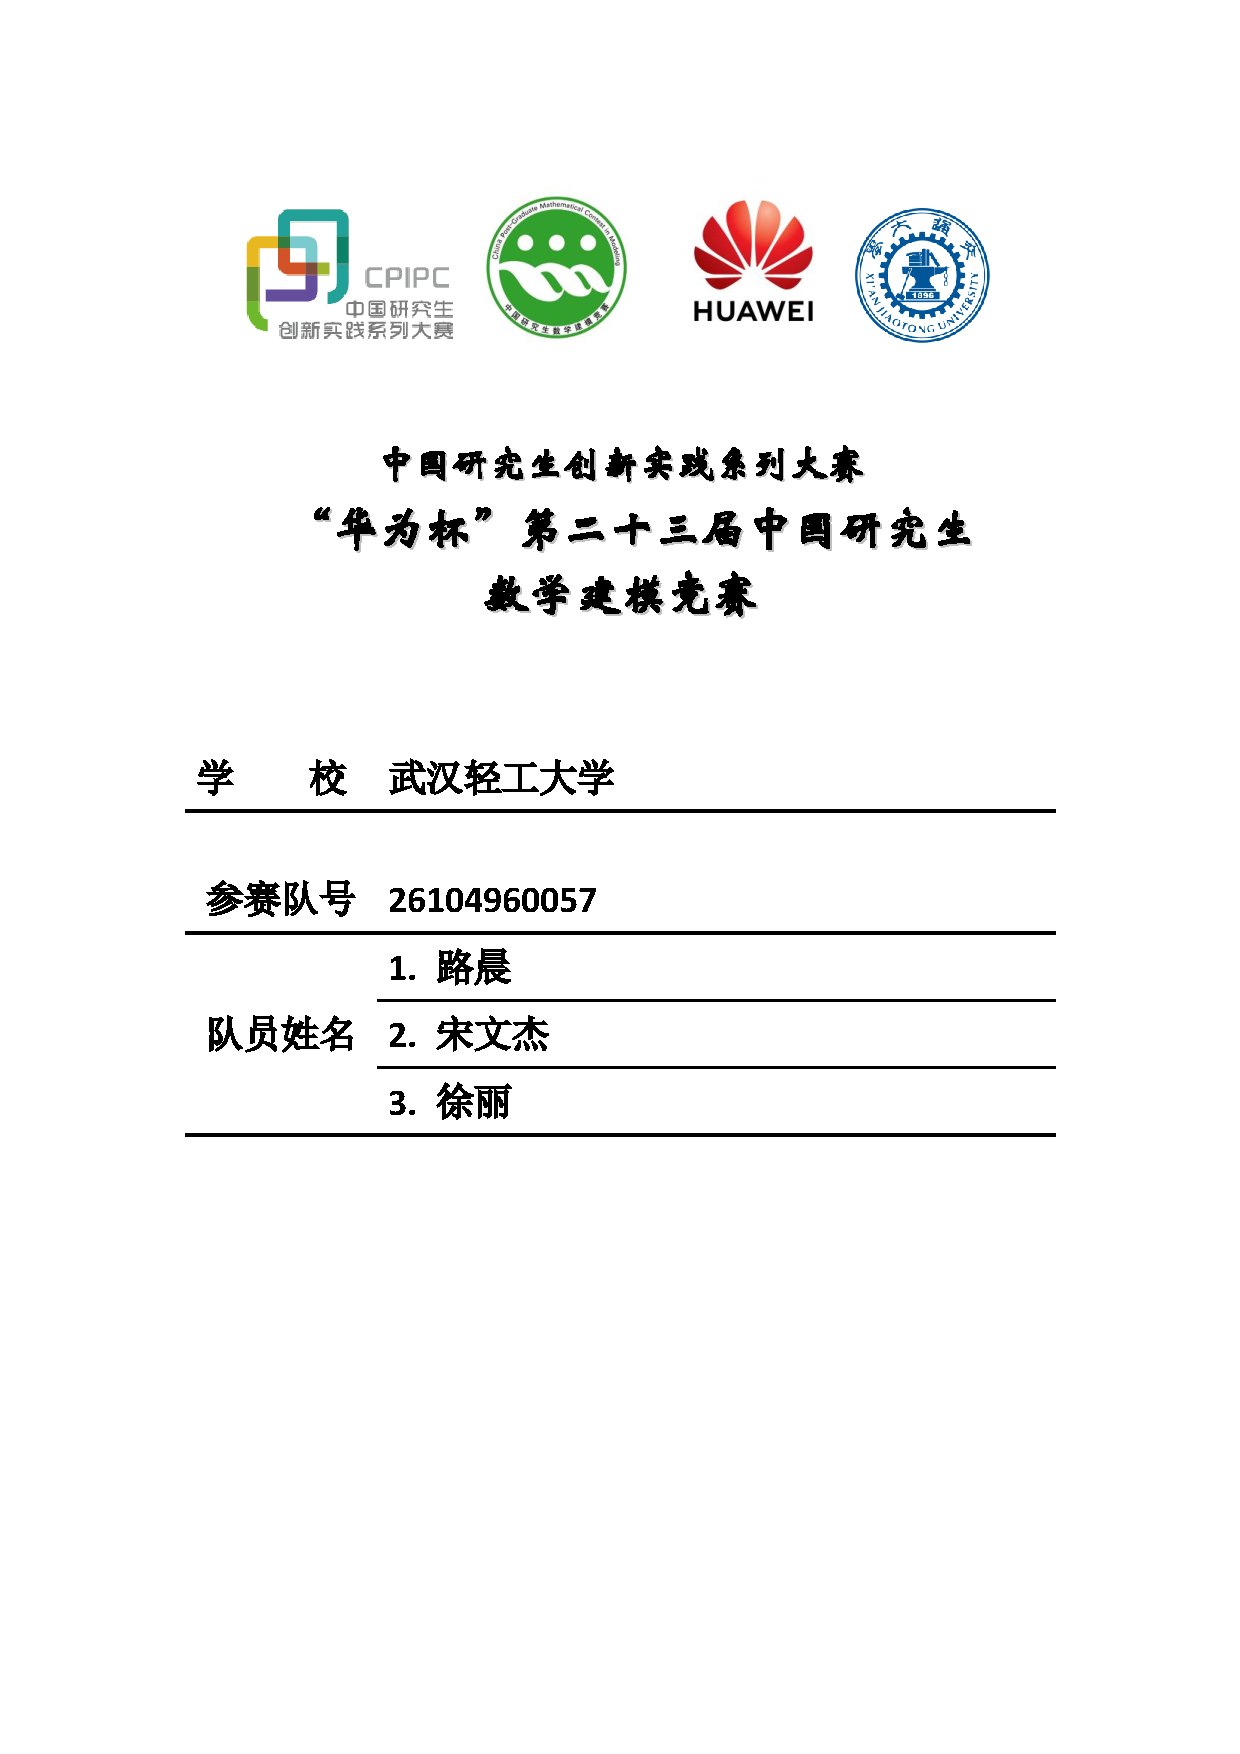
\includegraphics[width=\paperwidth,height=\paperheight]{frontmatter/official_cover.pdf}}}
\null\thispagestyle{empty}\clearpage
\pagenumbering{arabic}
\hypersetup{pageanchor=true}
\phantomsection\label{front:abstract}
\addcontentsline{toc}{section}{摘要}
\begin{center}
{\heiti\zihao{3}复杂场景下多模态情感识别的数学建模与算法设计\par}
\vspace{0.8\baselineskip}
{\heiti\zihao{4}摘\quad 要\par}
\end{center}
\noindent\hspace*{2em}多模态情感识别需要同时利用文本、语音和视觉信息，但三种模态的时间粒度与特征形式不同，原始特征难以直接对应；局部连续缺失会改变可用信息，影响情感分类与强度回归；预测结果还需要说明模型主要依赖哪些模态和局部输入。围绕这些问题，本文依次完成原始视频的三模态特征提取与时序对齐、连续缺失条件下的情感预测，以及模态贡献、模态交互和关键输入位置分析。

针对问题一，我们对附件1的100条原始视频分别提取文本、语音和视觉特征，采用的编码器依次为RoBERTa-base、WavLM-base-plus和SigLIP2-B/16。文本结合语音识别时间信息确定词语或片段的位置，语音由WAV采样范围恢复媒体时间，视觉按采样画面的真实显示时间确定对应区间。文本以词语或片段为单位，语音表示具有较高时间密度，视觉则来自离散采样画面，三种序列在相同索引处未必对应同一段视频内容。因此，时间对应以各观测所覆盖的真实媒体区间为依据，保留各模态原有的时间分布。以媒体时间为共同基准，将每条视频的有效时长划分为50个公共时间窗，按最大时间重叠选择对应的原生特征，同时保存有效掩码和来源记录。映射后各模态具有相同的序列长度，同时通过有效掩码和来源记录保留原始观测的覆盖情况与来源位置。最终得到文本、语音和视觉各$100\times50\times768$的特征数组，平均有效覆盖率分别为0.8242、0.9910和1.0000。典型样本回查表明，公共时间窗能够对应到文本片段、WAV采样范围和视频源帧。

针对问题二，我们使用附件2提供的50位对齐特征，同时预测三分类情感极性和连续情感强度。掩码均值池化模型MMP在有效位置上等权聚合，各模态表示经独立投影后拼接，分别进入分类头与回归头，作为分类与回归基线；考虑到不同位置的情感信息并不等量，在其上加入内容驱动的时间加权残差分支，得到轻量时间注意力残差池化模型LTARP。均值分支保留有效序列的整体信息，加权分支补充不同位置的内容差异，可学习残差系数控制补充表示的作用。分类与回归采用加权交叉熵和SmoothL1损失联合优化，使同一融合表示同时服务于极性判断和强度估计。该模型仅增加883个参数，总参数量为164343。从缺失模态、缺失位置和缺失比例三个方面构造54种连续局部缺失场景，比较完整输入与遮挡输入下的分类和回归结果。场景覆盖单模态及双模态缺失，分别考察连续信息损失发生在前段、中段或后段时的影响。评价同时采用宏平均F1、平均绝对误差MAE及Pearson相关系数，分别反映类别识别、连续强度误差和预测变化的一致程度。完整输入下，LTARP的宏平均F1、MAE和Pearson分别为0.6243、0.6052和0.6475；54种缺失场景平均下分别为0.6163、0.6086和0.6417。分模态结果显示，文本连续缺失带来的退化最明显，语音和视觉缺失的影响相对较小，表明三种信息在该组样本中的预测作用存在差异。为考察LTARP与不同多模态建模路线的相对表现，将11种公开方法适配到相同对齐特征和双任务输出接口。在本文统一输入与评价设置下，LTARP在约16.4万参数规模下保持了较高的宏平均F1，并兼顾连续强度预测和连续缺失场景表现。固定模型完成附件3全部30条无标签样本的情感极性与连续强度预测，输出对应的逐样本结果。

针对问题三，我们固定问题二的预测模型，枚举三种模态的全部8种输入组合并计算精确Shapley贡献，分别分析文本、语音和视觉对分类及回归输出的作用。分类分析围绕固定预测类别的对数优势展开，回归分析则围绕连续预测输出展开，从而分别描述各模态对两类任务的作用。进一步比较两两模态联合输入的贡献与简单可加组合，考察不同信息组合对当前预测目标的影响。交互正值表示联合输入的贡献高于可加组合，负值表示低于可加组合，以此区分单一模态作用与联合输入产生的额外变化。模态贡献和交互描述整路输入的作用，为进一步确定重要信息位于序列中的具体位置，在分类主导模态内采用连续窗口遮挡，保持其余输入不变，逐一比较候选区间被遮挡前后的输出，定位高影响位置。以随机等长窗口作为对照，使两类区间的输出变化在相同遮挡长度下进行比较；再通过删除实验观察逐步移除所选位置后的响应，检查关键位置分析与预测变化的一致性。独立验证子集中，遮挡所选窗口后的分类对数优势平均下降0.482771，随机等长窗口下降0.082036，差值为0.400735，按视频分组自助采样得到的95\%区间为$[0.3635,\,0.4372]$。所选区间被遮挡后对分类输出的影响明显大于随机等长区间。解释结果保留模态贡献、关键区间和对应输入来源：文本关键位置可以回查到原文字符区间，语音和视觉关键位置可以回查到相应未对齐特征行。最终完成附件4全部20条无标签样本的预测与解释，逐样本报告情感极性、连续强度、三模态贡献和关键输入区间。

综上，三模态特征能够在统一时间位置上保留原始来源对应关系，LTARP以较小参数增量完成局部连续缺失条件下的情感分类与强度回归，Shapley贡献和连续遮挡进一步确定预测依赖的模态与关键输入位置。所得到的结果覆盖原始特征构建、无标签样本预测和输入作用分析，并保留了可供逐样本核对的来源信息，为复杂场景下多模态情感识别提供了具体方法及可复现结果。

\par\vspace{0.7\baselineskip}
\noindent\textbf{关键词：}多模态情感识别；时序对齐；局部连续缺失；情感预测；Shapley值；可解释分析

\clearpage
\tableofcontents
\clearpage
\setcounter{section}{2}
\section{问题一：多模态特征提取与时序对齐}\label{sec:q1}

\subsection{问题分析与总体方案}\label{subsec:q1_framework}
\QOneParagraph 附件1给出了100条包含文本、语音和画面信息的视频样本。三种模态经过各自编码后，文本以词语或片段形成表示，语音形成较密集的声学序列，视觉对应离散采样帧。要将这些长度和时间粒度不同的序列组织在一起，首先需要确定每个特征在原视频中对应的时间范围。

\QOneParagraph 本文把独立编码、尚未进入公共时间轴的向量序列称为{\songti 原生特征}，把每个向量对应的媒体时间区间称为它的{\songti 时间支持}。文本的时间支持来自词语或识别片段，语音来自WAV样本范围，视觉来自采样帧附近的区间。这样，每个向量既保留内容表示，也带有能够连接其他模态的时间信息。

\QOneParagraph 整体方案如图~\ref{fig:fig01_q1_overview}所示。先建立统一媒体时间基准，分别提取带时间支持的三模态原生特征，再将每条视频的有效时长划分为50个公共窗。各模态按最大时间重叠规则选取每个窗的来源，形成统一长度的序列，并同步保存有效掩码和原始来源记录。

\begin{figure}[htbp]
\centering
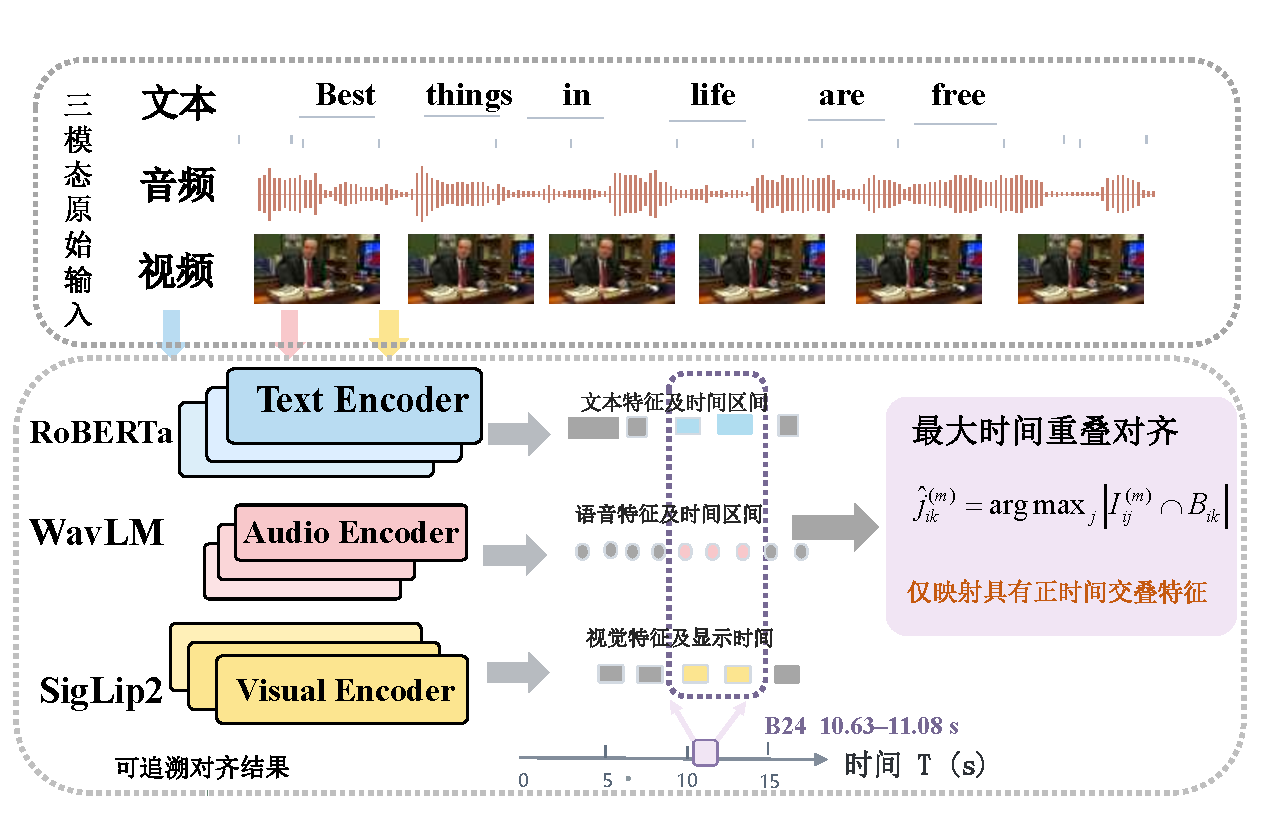
\includegraphics[width=1.0\textwidth]{figures/q1/fig01_q1_overview.pdf}
\caption{三模态特征提取与时序对齐流程。}
\label{fig:fig01_q1_overview}
\end{figure}

\subsection{原始数据预处理与统一时间基准}\label{subsec:q1_timeline}
\QOneParagraph 三模态的时间联系从原始媒体开始建立。每条样本以视频标识和片段编号定位，将附件1文件夹名、MP4文件名与\texttt{label-100.xlsx}中的记录连接，取得对应的赛题转写与情感标注。媒体路径及文件哈希随处理记录保存，使三种特征始终连接到同一片段。

\QOneParagraph 音频由FFmpeg提取MP4的第一音轨，转换为16 kHz单声道PCM WAV；视频帧的显示时间戳（PTS）由FFprobe读取。对全部100条媒体核验后，音视频流起点、首视频帧PTS和首解码音频帧PTS均为0 s，因而WAV样本零点与视频PTS零点共同构成相对时间起点。

\QOneParagraph 以容器时长和最后一帧PTS加一个名义帧间隔中的较大者作为有效时长$T_i$，第$i$条样本的媒体时间域为
\begin{equation}
\mathcal{T}_i=[0,T_i).
\label{eq:q1_timeline}
\end{equation}
\QOneParagraph 文本时间、WAV样本位置换算的秒数及视频帧PTS都在媒体时间域$\mathcal{T}_i$中记录。为得到统一长度的序列，将每条样本自身的有效时长等分为$K=50$个公共窗，并保存各窗的实际秒数边界。由于视频长度不同，同一窗号的时间范围随样本时长变化。

\QOneParagraph 图~\ref{fig:fig05_q1_data_statistics}中，视频时长以较短片段为主，同时包含少量较长片段。文本有效窗数的样本间差异较大，语音和视觉则较集中；文本内容主要采用赛题转写，时间戳回退涉及少数样本。这些差异在共同时间基准下保留，成为逐样本特征记录的一部分。

\begin{figure}[htbp]
\centering
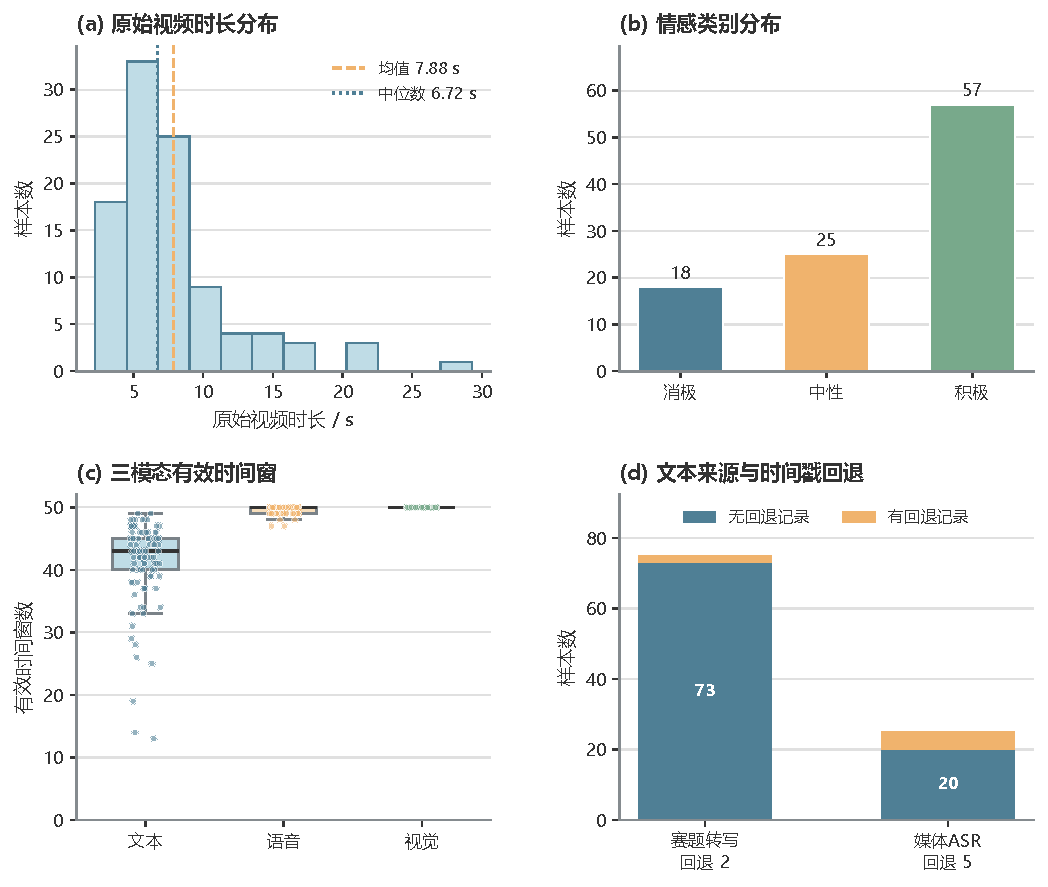
\includegraphics[width=0.98\textwidth]{figures/q1/fig05_q1_data_statistics.pdf}
\caption{附件1样本与三模态特征统计。}
\label{fig:fig05_q1_data_statistics}
\end{figure}

\subsection{三模态原生特征提取}\label{subsec:q1_native}
\QOneParagraph 有了共同的媒体时间坐标，就可以分别为词语、声学位置和采样画面建立时间支持。三种模态各自编码，原生序列保留自身采样密度，每一行向量与对应时间区间及原始来源一起保存。

\subsubsection{文本特征提取}\label{subsubsec:q1_text}
\QOneParagraph 文本的内容和时间信息分别来自赛题转写与同一视频的语音识别。采用Whisper large-v3-turbo获取词级和片段级时间\cite{radford2023whisper}，将能够对应到识别词序的赛题词语连接到这些区间；未匹配词保留在原转写中，编码时使用已建立时间支持的词语。对于文本对应条件不满足的片段，采用媒体ASR内容。最终\QOneOfficialTextCount 条使用赛题转写，\QOneMediaAsrCount 条使用媒体ASR。例如，样本\texttt{\detokenize{-NFrJFQijFE__2}}的赛题转写描述仪器准备，而识别内容描述鹰的听觉和视觉，该样本采用媒体ASR，同时保留原转写。

\QOneParagraph 词级区间须为有限值，满足$0\leq s<e\leq T_i$，且起止边界相对于前一原始词区间保持时间顺序。无效或非单调的词级区间回退到所属识别片段的有效范围；若该片段也无有效时间，则记录为未解决。时间来源和回退标记随文本记录保存，区分词级和片段级支持。

\QOneParagraph 带时间信息的词语列表按图~\ref{fig:fig02_q1_text_feature_extraction}的流程送入RoBERTa-base编码\cite{liu2019roberta}。快速分词器按预分词列表处理，最大长度为510词元；取最后一层隐藏表示，并按词索引平均同一词的子词向量，得到768维原生表示。特殊词元由分词器索引排除，截断后没有对应词元的单元保留提示记录。模型使用预训练权重进行推理。第$j$个文本特征及其时间支持为
\begin{equation}
\mathbf h_{ij}^{(T)}\in\mathbb R^{\QOneTextDim},\qquad
I_{ij}^{(T)}=[s_{ij}^{(T)},e_{ij}^{(T)}).
\label{eq:q1_text_feature}
\end{equation}

\begin{figure}[!htbp]
\centering
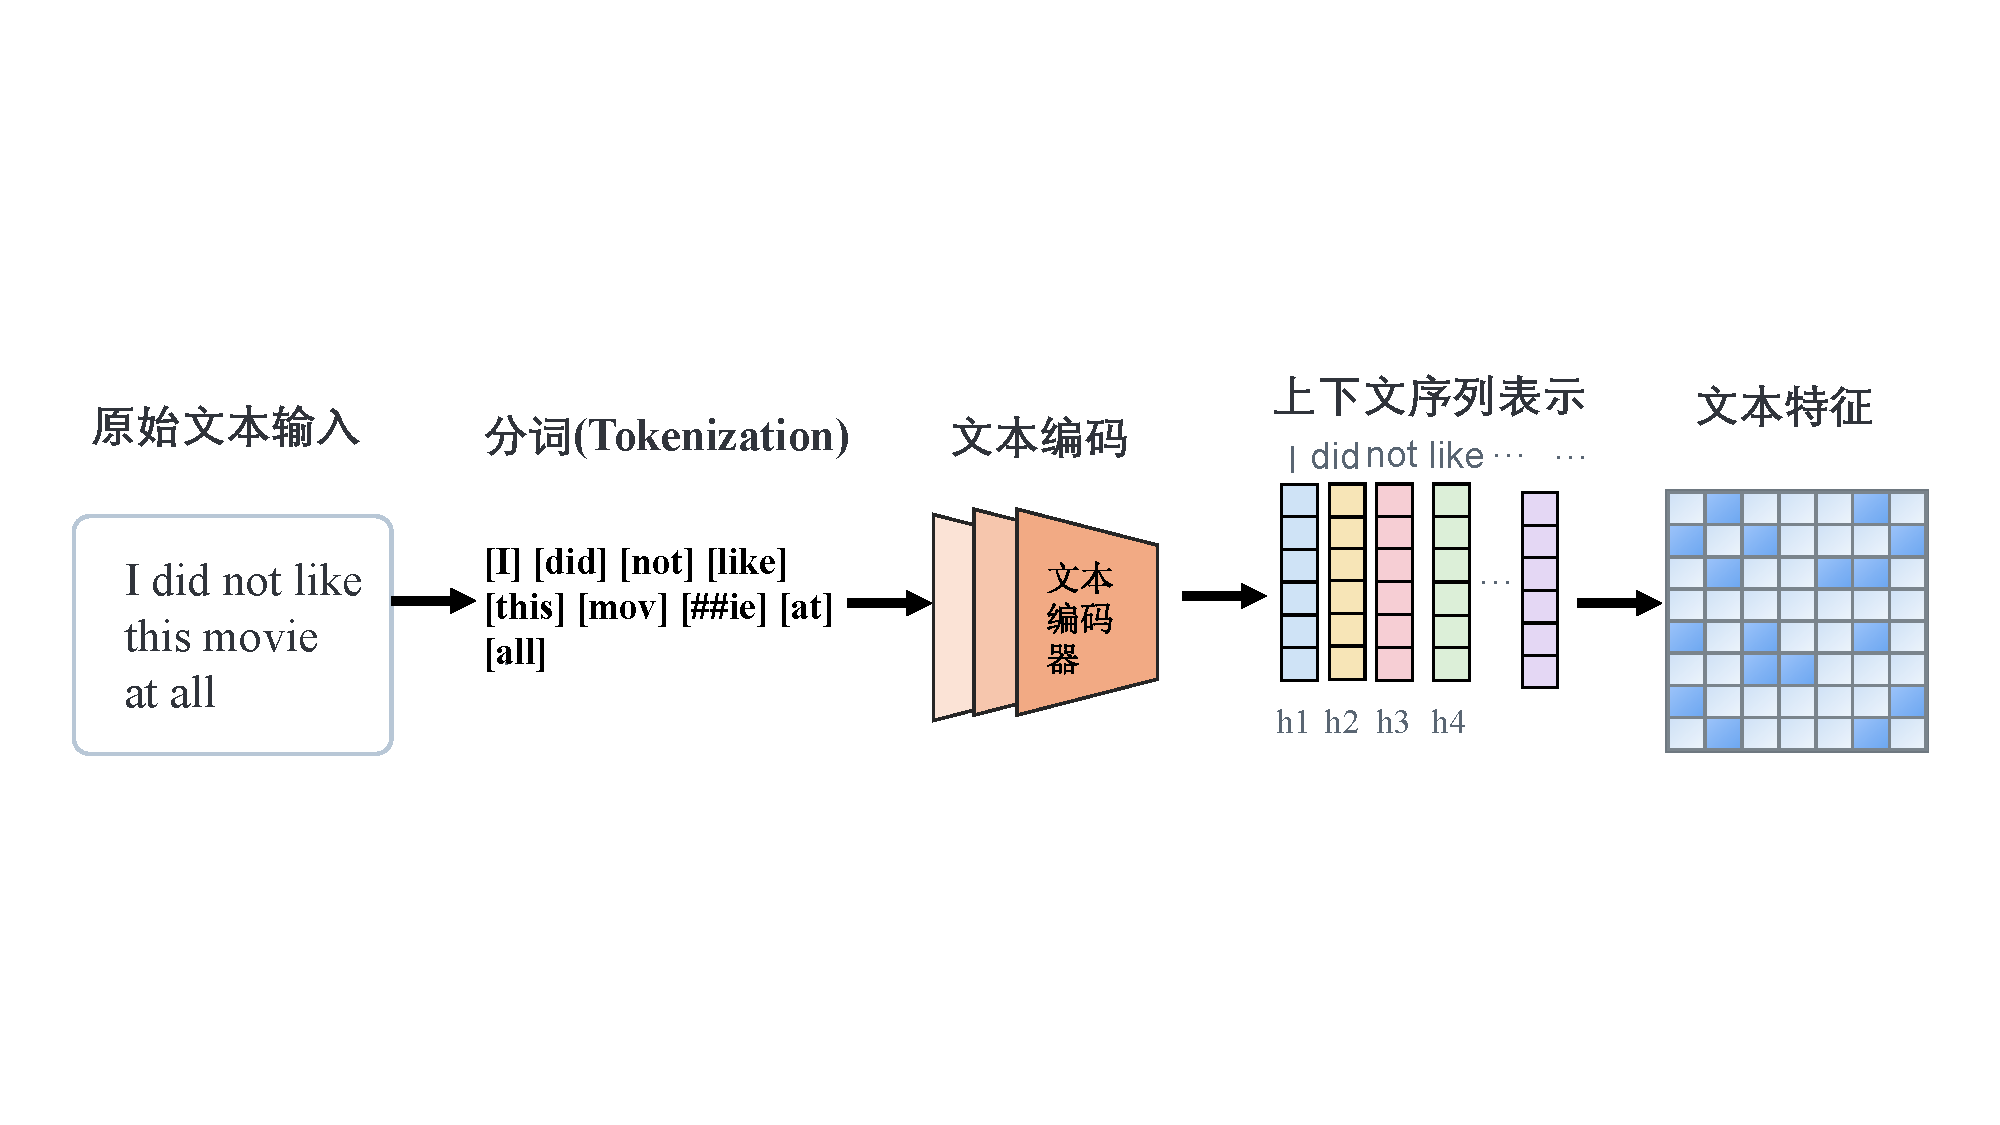
\includegraphics[trim=30bp 145bp 30bp 145bp,clip,width=.94\textwidth]{figures/q1/fig02_q1_text_feature_extraction.pdf}
\caption{文本模态特征提取流程。色块为表示结构示意。}
\label{fig:fig02_q1_text_feature_extraction}
\end{figure}
\FloatBarrier

\subsubsection{语音特征提取}\label{subsubsec:q1_audio}
\QOneParagraph 文本建立了语言内容的时间位置，语音则需将连续波形编码后的声学位置连接回WAV。使用WavLM-base-plus处理16 kHz单声道输入\cite{chen2022wavlm}，取最后一层逐位置表示，得到768维声学序列。

\QOneParagraph 根据模型卷积核与步长，计算累计步距$H$和感受范围$R$。当WAV含$N$个样本时，第$j$个声学位置对应采样区间$[jH,\min(N,jH+R))$；区间端点除以采样率后转换为秒，并将末端限制在$T_i$以内。输出位置数与模型长度计算函数核对，原生向量同时记录其WAV采样范围。声学特征及时间支持记为
\begin{equation}
\mathbf h_{ij}^{(A)}\in\mathbb R^{\QOneAudioDim},\qquad
I_{ij}^{(A)}=[s_{ij}^{(A)},e_{ij}^{(A)}).
\label{eq:q1_audio_feature}
\end{equation}
\QOneParagraph 声学位置较密集，同一个公共窗内可能覆盖多个原生区间，后续通过时间交叠确定该窗的语音来源。原始波形到声学表示的处理见图~\ref{fig:fig03_q1_audio_feature_extraction}。

\begin{figure}[!htbp]
\centering
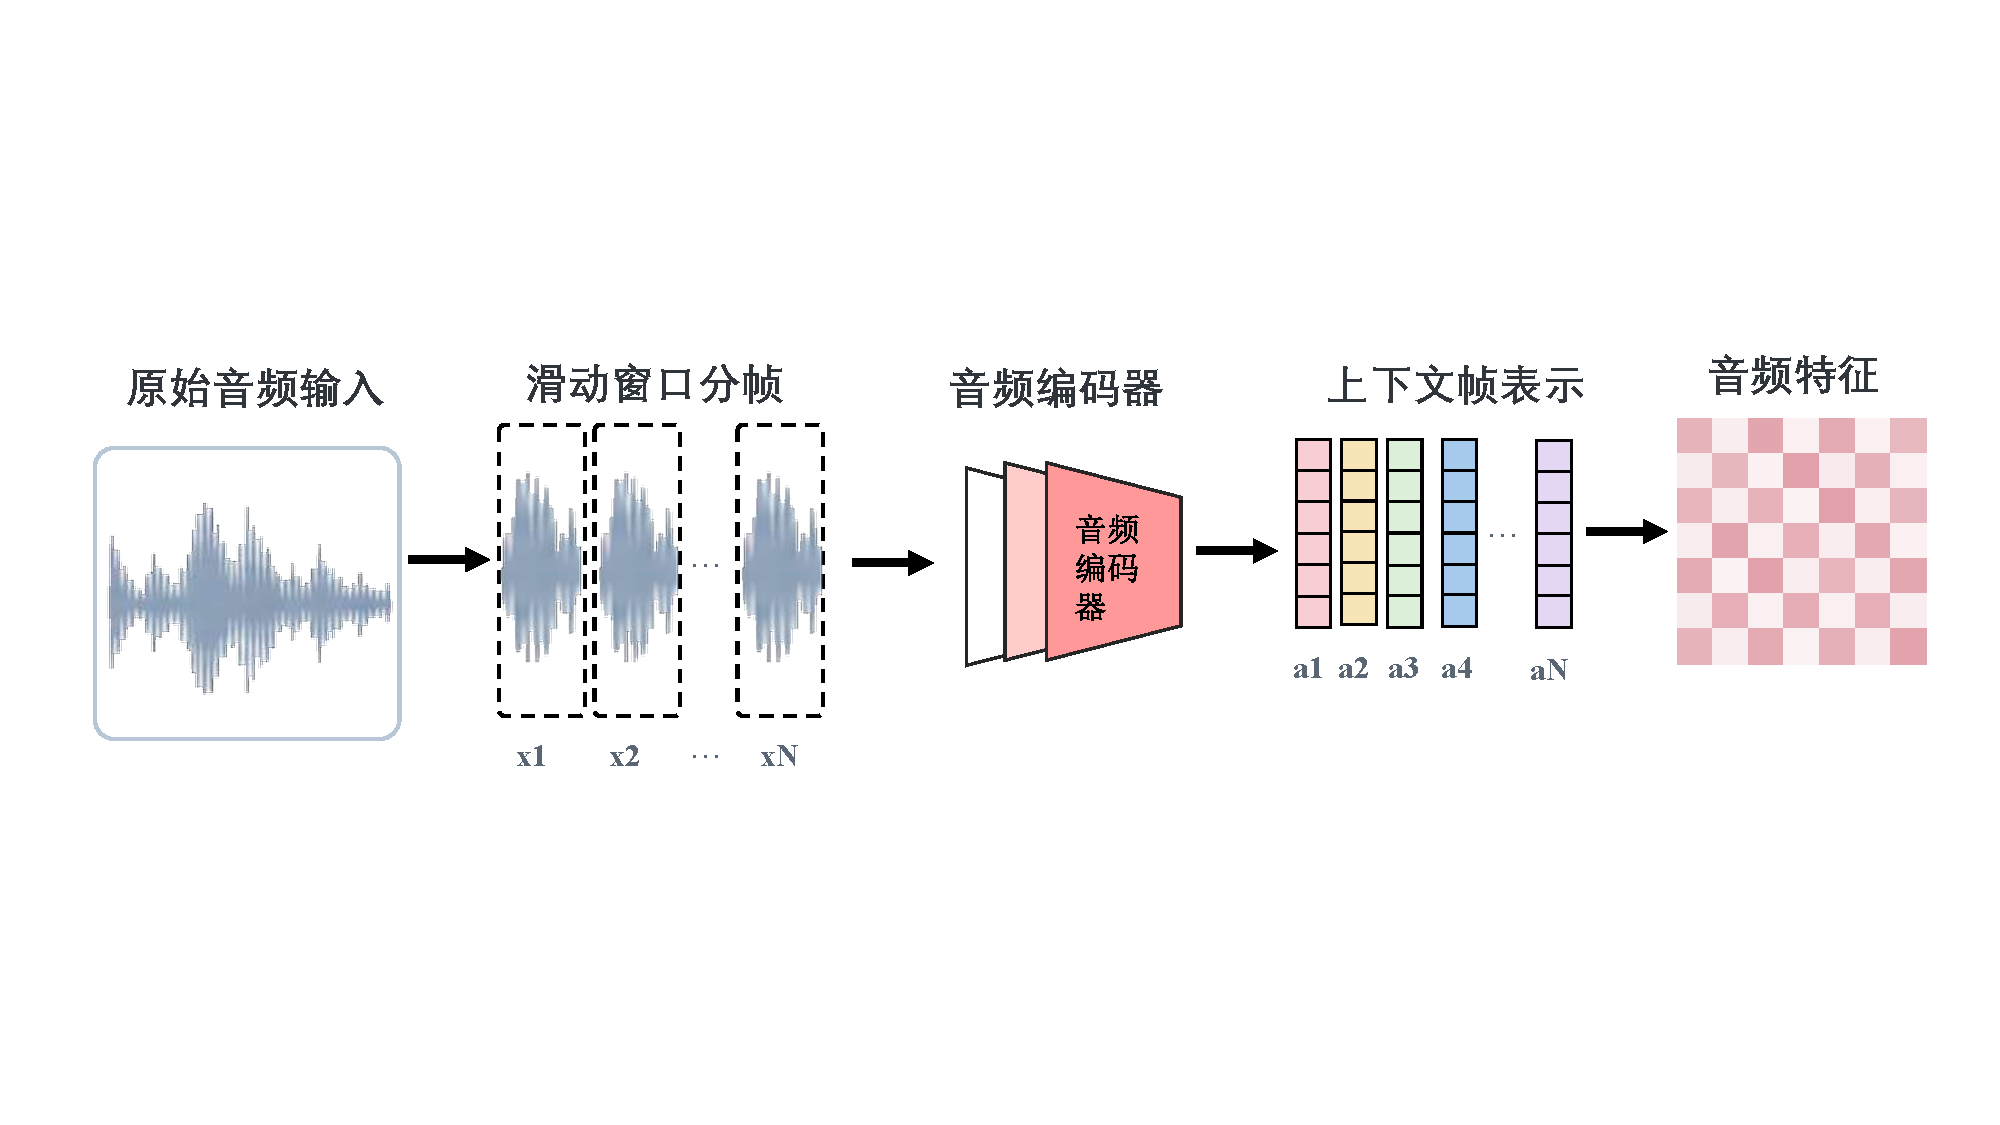
\includegraphics[trim=30bp 145bp 30bp 145bp,clip,width=.94\textwidth]{figures/q1/fig03_q1_audio_feature_extraction.pdf}
\caption{语音模态特征提取流程。色块为表示结构示意。}
\label{fig:fig03_q1_audio_feature_extraction}
\end{figure}
\FloatBarrier

\subsubsection{视觉特征提取}\label{subsubsec:q1_vision}
\QOneParagraph 文本和语音已有媒体时间区间，视觉特征进一步由采样画面的真实显示时刻定位。以每秒4帧建立目标时间网格，在PTS序列中选择离目标时刻最近的帧；等距时取较早帧，相邻目标选中同一帧时保留一次。所选画面按源帧编号解码，经配套图像处理器缩放、归一化后，送入SigLIP2-base-patch16-224\cite{tschannen2025siglip2}，得到768维视觉向量。

\QOneParagraph 以相邻已选帧PTS的中点划分支持区间，首边界为0，尾边界为$T_i$。每个向量同时保留源帧编号和PTS：前者定位原视频画面，后者记录其显示时刻，支持区间则参与公共窗映射。视觉原生表示为
\begin{equation}
\mathbf h_{ij}^{(V)}\in\mathbb R^{\QOneVisionDim},\qquad
I_{ij}^{(V)}=[s_{ij}^{(V)},e_{ij}^{(V)}).
\label{eq:q1_vision_feature}
\end{equation}
\QOneParagraph 全部视频的顺序解码帧与FFprobe记录的显示时间经核验保持一致，源帧编号与PTS可以联合回查视觉来源。采样与编码步骤见图~\ref{fig:fig04_q1_video_feature_extraction}。

\begin{figure}[!htbp]
\centering
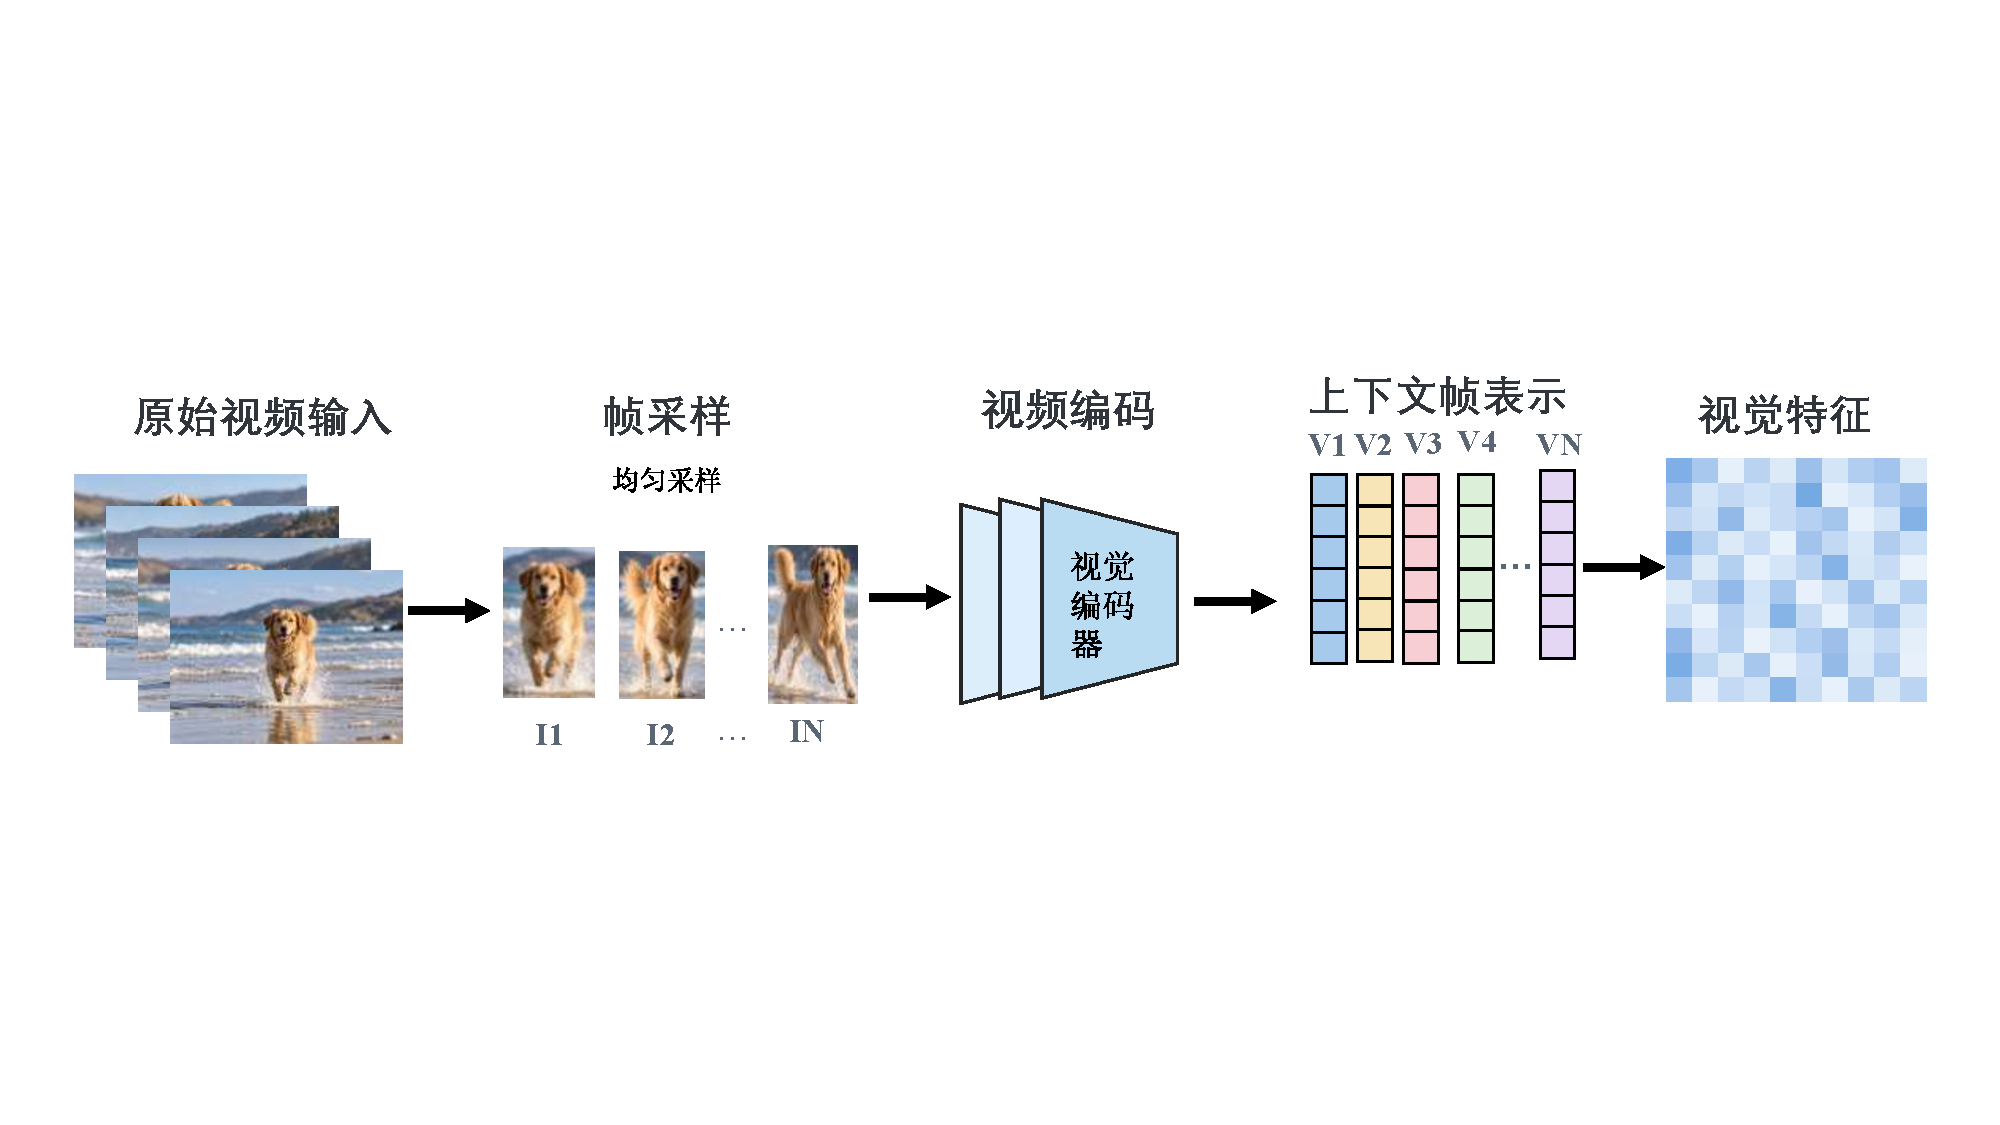
\includegraphics[trim=30bp 145bp 30bp 145bp,clip,width=.94\textwidth]{figures/q1/fig04_q1_video_feature_extraction.pdf}
\caption{视觉模态特征提取流程。色块为表示结构示意。}
\label{fig:fig04_q1_video_feature_extraction}
\end{figure}
\FloatBarrier

\subsection{基于最大时间重叠的跨模态时序对齐}\label{subsec:q1_alignment}
\QOneParagraph 经过独立提取，三种模态都具有原生向量和时间支持。跨模态对齐据此将它们映射为固定长度序列，使同一公共位置汇集来自相同媒体时间范围的文本、语音和视觉信息（图~\ref{fig:fig06_q1_temporal_alignment}）。

\QOneParagraph 一个公共窗可与同一模态的多个原生区间交叠。本文选取正交叠时长最长的一个，让该窗直接继承对应向量；这样，每个有效位置都连接到一个确定的原生来源。

\QOneParagraph 将第$i$条样本的有效时长均分为$K=\QOneBins$个半开区间：
\begin{equation}
B_{ik}=\left[\frac{kT_i}{K},\frac{(k+1)T_i}{K}\right),\qquad k=0,1,\ldots,K-1.
\label{eq:q1_bins}
\end{equation}
记$b_{ik}=kT_i/K$，模态$m\in\{T,A,V\}$的原生时间支持为
\begin{equation}
I_{ij}^{(m)}=[s_{ij}^{(m)},e_{ij}^{(m)}).
\label{eq:q1_native_interval}
\end{equation}
其与公共窗的交叠长度为
\begin{equation}
\omega_{ijk}^{(m)}=\max\left(0,\min(e_{ij}^{(m)},b_{i,k+1})-\max(s_{ij}^{(m)},b_{ik})\right).
\label{eq:q1_overlap}
\end{equation}
当存在正交叠时，选择
\begin{equation}
j_{ik}^{(m)}=\arg\max_j\omega_{ijk}^{(m)},\qquad \omega_{i,j_{ik}^{(m)},k}^{(m)}>0,
\label{eq:q1_argmax}
\end{equation}
并令
\begin{equation}
\mathbf z_{ik}^{(m)}=\mathbf h_{i,j_{ik}^{(m)}}^{(m)},\qquad M_{ik}^{(m)}=1.
\label{eq:q1_hard_feature}
\end{equation}

\QOneParagraph 实际实现中，最大交叠并列时，优先选择区间中心更接近公共窗中心者，仍并列则取较早原生索引。所选索引、时间支持和实际交叠时长写入来源记录。无正交叠时，令$\mathbf z_{ik}^{(m)}=\mathbf0$、$M_{ik}^{(m)}=0$，保留空来源；有效性由掩码$M_{ik}^{(m)}$表示。单样本及全量结果分别组织为
\begin{equation}
\mathbf Z_i^{(m)}\in\mathbb R^{\QOneBins\times d_m},\qquad
\mathcal Z^{(m)}\in\mathbb R^{\QOneSamples\times\QOneBins\times d_m},\quad d_T=d_A=d_V=768.
\label{eq:q1_tensor_shape}
\end{equation}

\begin{figure}[htbp]
\centering
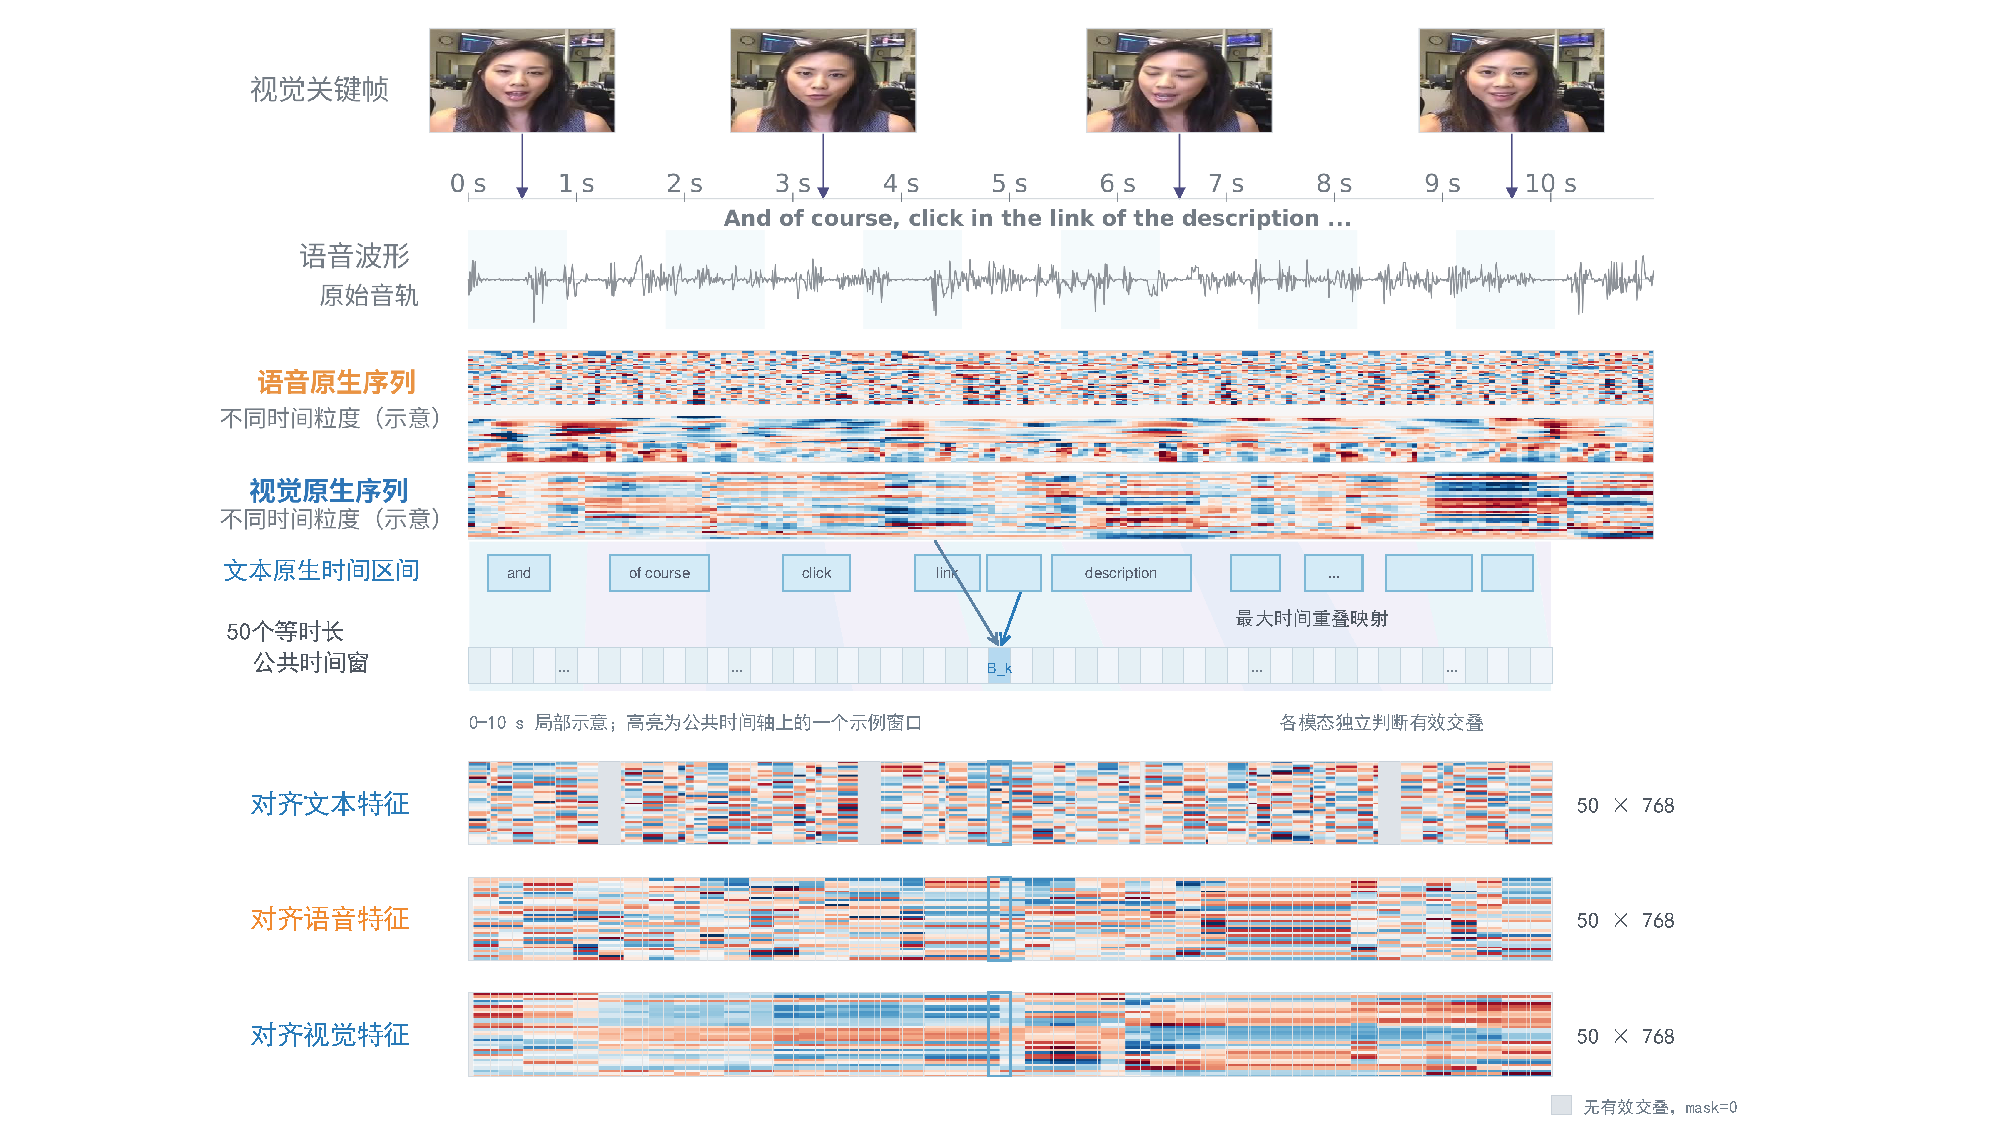
\includegraphics[trim=100bp 0bp 130bp 0bp,clip,width=1.0\textwidth]{figures/q1/fig06_q1_temporal_alignment.pdf}
\caption{三模态原生序列到公共时间窗的映射。矩阵色值为结构示意。}
\label{fig:fig06_q1_temporal_alignment}
\end{figure}
\FloatBarrier

\subsection{特征构建结果与完整性检验}\label{subsec:q1_validation}
\QOneParagraph 对全部\QOneSamples 条样本完成映射后，文本、语音和视觉各形成$100\times50\times768$的单精度浮点数组，有效掩码各为$100\times50$的布尔数组。三种模态的原生向量总数及平均覆盖率见表~\ref{tab:q1_feature_scheme}。

\begin{table}[htbp]
\centering\zihao{-4}
\caption{三模态特征构建与时间覆盖结果}
\label{tab:q1_feature_scheme}
\begin{tabularx}{\textwidth}{@{}lXcccr@{}}
\toprule
模态 & 特征提取方法 & \shortstack{原生\\特征数} & \shortstack{特征\\维数} & \shortstack{单样本\\对齐形状} & \shortstack{平均时间\\覆盖率} \\
\midrule
文本 & \texttt{RoBERTa-base} & 1847 & 768 & $\QOneBins\times768$ & 0.8242 \\
语音 & \texttt{WavLM-base-plus} & 38776 & 768 & $\QOneBins\times768$ & 0.9910 \\
视觉 & \texttt{SigLIP2-B/16} & 3205 & 768 & $\QOneBins\times768$ & 1.0000 \\
\bottomrule
\end{tabularx}
\end{table}


\QOneParagraph 文本、语音和视觉的有效位置分别为4121、4955和5000，平均覆盖率为\QOneTextCoverage、\QOneAudioCoverage 和\QOneVisionCoverage。文本以离散词语和片段出现，部分公共窗内没有对应文本特征，由文本掩码标记；连续声学序列更密集，语音仅在少数位置出现空窗；视觉支持区间覆盖全部50窗。覆盖率差异由各模态的时间组织体现出来。

\QOneParagraph 完整性检查确认100个样本编号唯一，矩阵行序与样本清单一致，三模态数组形状及掩码尺寸匹配，特征数值均有限，无效位置均为零。来源表包含全部15000个“样本—公共窗—模态”组合，每个有效位置均能连接到被选原生索引及原始来源。

\subsection{全量样本特征构建结果}\label{subsec:q1_all_samples}
\QOneParagraph 不同样本在视频时长、文本来源和有效窗覆盖上存在明显差异。表~\ref{tab:q1_all_samples}选取8条具有代表性的样本，覆盖不同视频长度、文本来源、有效窗数量和时间戳回退情况；附件1全部100条样本的对应结果见附录A表~\ref{tab:q1_all_samples_appendix}。

\begin{table}[H]
\centering\zihao{-4}
\caption{代表性样本的三模态特征构建与时序对齐结果}\label{tab:q1_all_samples}
\setlength{\tabcolsep}{2pt}
\renewcommand{\arraystretch}{1.08}
\begin{tabular}{@{}>{\raggedright\arraybackslash}p{4.1cm}>{\centering\arraybackslash}p{1.25cm}>{\centering\arraybackslash}p{1.15cm}>{\centering\arraybackslash}p{2.25cm}>{\centering\arraybackslash}p{1.3cm}>{\centering\arraybackslash}p{2.3cm}>{\centering\arraybackslash}p{1.9cm}>{\centering\arraybackslash}p{.9cm}@{}}
\toprule
样本ID & 时长/s & 模态 & \shortstack{维度\\(T/A/V)} & \shortstack{对齐\\粒度} & \shortstack{有效窗\\(T/A/V)} & \shortstack{文本\\来源} & 回退\\
\midrule
\texttt{\detokenize{-a55Q6RWvTA__3}} & 22.154 & T/A/V & 768/768/768 & 50窗 & 48/50/50 & 赛题转写 & 0\\
\texttt{\detokenize{-NFrJFQijFE__1}} & 5.746 & T/A/V & 768/768/768 & 50窗 & 13/50/50 & 媒体ASR & 5\\
\texttt{\detokenize{-yRb-Jum7EQ__1}} & 29.288 & T/A/V & 768/768/768 & 50窗 & 38/50/50 & 媒体ASR & 8\\
\texttt{\detokenize{-mJ2ud6oKI8__9}} & 7.033 & T/A/V & 768/768/768 & 50窗 & 49/50/50 & 媒体ASR & 1\\
\texttt{\detokenize{-9y-fZ3swSY__4}} & 2.821 & T/A/V & 768/768/768 & 50窗 & 44/47/50 & 赛题转写 & 0\\
\texttt{\detokenize{-RfYyzHpjk4__2}} & 5.516 & T/A/V & 768/768/768 & 50窗 & 42/49/50 & 赛题转写 & 1\\
\texttt{\detokenize{-3g5yACwYnA__13}} & 5.514 & T/A/V & 768/768/768 & 50窗 & 33/49/50 & 赛题转写 & 0\\
\texttt{\detokenize{-t217m2on-s__7}} & 17.183 & T/A/V & 768/768/768 & 50窗 & 48/50/50 & 赛题转写 & 0\\
\bottomrule
\end{tabular}
\end{table}
\par\vspace{0.2em}\noindent\begin{minipage}{\textwidth}{\zihao{-4}\noindent 注：\par
\begin{enumerate}[label=(\arabic*),leftmargin=2.4em,labelsep=.4em,itemsep=0pt,topsep=0pt,parsep=0pt]
\item T、A、V分别表示文本、语音、视觉；“有效窗(T/A/V)”依次给出三模态的有效公共窗数。
\item “赛题转写”为附件1 \texttt{label-100.xlsx} 的text字段；“媒体ASR”为当前视频语音识别得到的文本。
\item “回退”为词级时间戳不可用时，实际采用所属识别片段时间区间的映射次数。
\end{enumerate}}\end{minipage}


\QOneParagraph 文本有效窗数为13--49，语音为47--50，视觉均为50，文本时间支持呈现出最明显的样本间差异。75条采用赛题转写，25条采用媒体ASR；7条样本包含时间戳回退，累计21个实际回退位置。逐样本记录因而同时呈现覆盖范围和文本时间支持的粒度，与总体平均覆盖率共同反映特征构建结果。
\FloatBarrier

\subsection{方案比较与信息保持能力验证}\label{subsec:q1_analysis}
\QOneParagraph 在确认特征能够完整读取并回溯后，进一步比较不同方案对情感信息的保持能力。使用固定的轻量预测模型作为特征探针，在同一训练与评价设置下分别改变对齐方法、视觉编码器和模态组合，以准确率、宏平均F1、MAE及皮尔逊相关系数观察差异。

\QOneParagraph 探针将每模态768维输入映射为32维，在公共位置拼接三路表示，经小型感知机变换和联合有效位均值池化，输出情感类别与连续强度。采用40轮AdamW训练，学习率0.002、权重衰减0.001，目标为交叉熵加0.25倍平滑绝对误差；标准化参数由各训练折的有效位置估计。评价为5次重复分层五折，表中报告均值与样本标准差。由于按片段标签分层、未按原视频分组，该实验用于Q1内部方案比较。

\subsubsection{时序对齐方法比较}\label{subsubsec:q1_align_ablation}
\QOneParagraph 首先比较最大时间重叠、最近中心和重叠加权平均，结果见表~\ref{tab:q1_alignment_ablation}及图~\ref{fig:fig07_q1_alignment_method_comparison}。三种方案的平均指标总体接近，最近中心在部分指标上略高；同时，其\QOneNearestZeroOverlap 个有效文本公共窗选择了与目标窗零交叠的来源。

\begin{table}[H]
\centering
\caption{不同时序对齐方法的定量比较}
\label{tab:q1_alignment_ablation}
\zihao{-4}
\setlength{\tabcolsep}{2pt}
\begin{tabular}{@{}>{\centering\arraybackslash}p{2.6cm}*{4}{>{\centering\arraybackslash}p{3.0cm}}@{}}
\toprule
对齐方法 & 准确率 & 宏平均 F1 值 & \shortstack{平均绝对误差\\（MAE）} & \shortstack{皮尔逊\\相关系数} \\
\midrule
\shortstack{最大时间\\重叠法} & \shortstack{0.6129\\$\pm$ 0.0938} & \shortstack{0.4816\\$\pm$ 0.0850} & \shortstack{0.5258\\$\pm$ 0.0966} & \shortstack{0.5419\\$\pm$ 0.1470} \\
\shortstack{最近中心法} & \shortstack{0.6148\\$\pm$ 0.0913} & \shortstack{0.4832\\$\pm$ 0.0849} & \shortstack{0.5210\\$\pm$ 0.0967} & \shortstack{0.5535\\$\pm$ 0.1492} \\
\shortstack{重叠加权\\平均法} & \shortstack{0.6074\\$\pm$ 0.0945} & \shortstack{0.4712\\$\pm$ 0.0868} & \shortstack{0.5237\\$\pm$ 0.0977} & \shortstack{0.5482\\$\pm$ 0.1506} \\
\bottomrule
\end{tabular}
\par\smallskip\noindent\zihao{-4} 注：数值为均值$\pm$样本标准差。
\end{table}


\QOneParagraph 重叠加权平均将多个原生向量合成为一个公共位置，来源随之变为多行向量及权重的组合。最大时间重叠则保留正时间交叠与单一来源，使每个公共位置能够直接回查到原生行。综合辅助评价、时间对应和回查方式，最终采用最大时间重叠对齐。

\begin{figure}[!htbp]
\centering
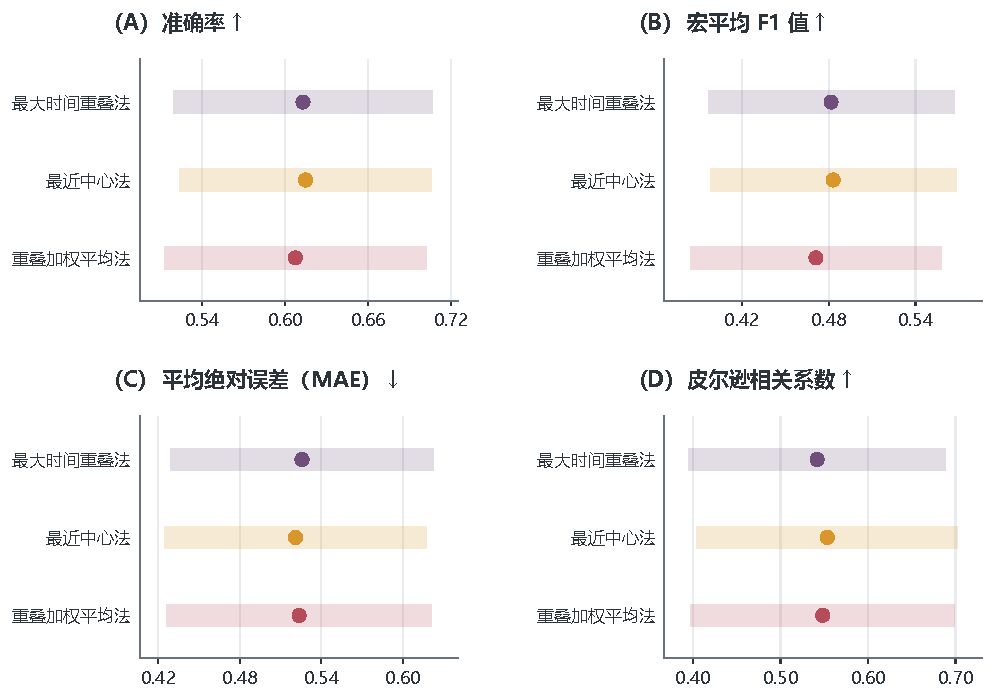
\includegraphics[width=0.98\textwidth]{figures/q1/fig07_q1_alignment_method_comparison.pdf}
\caption{对齐方法的辅助评价。点为均值，半透明区间为均值上下一个样本标准差。}
\label{fig:fig07_q1_alignment_method_comparison}
\end{figure}
\FloatBarrier

\subsubsection{视觉特征提取方法比较}\label{subsubsec:q1_vision_ablation}
\QOneParagraph 确定时间映射后，比较不同视觉表示对情感信息的保持效果。固定采样帧、PTS及对齐规则，仅将SigLIP2替换为DINOv3\cite{simeoni2025dinov3}，得到表~\ref{tab:q1_visual_backbone}的结果。

\begin{table}[htbp]
\centering
\caption{不同视觉特征提取方法的比较}
\label{tab:q1_visual_backbone}
\zihao{-4}
\setlength{\tabcolsep}{2pt}
\begin{tabular}{@{}p{2.3cm}*{4}{>{\centering\arraybackslash}p{2.9cm}}>{\centering\arraybackslash}p{1.7cm}@{}}
\toprule
视觉编码器 & 准确率 & \shortstack{宏平均\\F1} & MAE & 皮尔逊 r & \shortstack{提取时长\\（秒）} \\
\midrule
SigLIP2 & \shortstack{0.6129\\$\pm$ 0.0938} & \shortstack{0.4816\\$\pm$ 0.0850} & \shortstack{0.5258\\$\pm$ 0.0966} & \shortstack{0.5419\\$\pm$ 0.1470} & 52.37 \\
\shortstack{DINOv3\\（ViT-B/16）} & \shortstack{0.5899\\$\pm$ 0.0857} & \shortstack{0.4427\\$\pm$ 0.0760} & \shortstack{0.5401\\$\pm$ 0.0819} & \shortstack{0.5155\\$\pm$ 0.1473} & 70.38 \\
\bottomrule
\end{tabular}
\end{table}


\QOneParagraph SigLIP2的准确率、宏平均F1和相关系数均值更高，MAE均值更低，单次提取耗时也较短，因此选为最终视觉编码器。两组使用相同视觉来源，差异体现这些画面经不同骨干形成的表示效果。
\FloatBarrier

\subsubsection{模态组合比较}\label{subsubsec:q1_modality_ablation}
\QOneParagraph 在所选对齐方法与视觉编码器下，再比较三个单模态、三种双模态及三模态组合，结果见表~\ref{tab:q1_modality_ablation}。各组合沿用相同公共窗与有效位，通过增减输入观察任务信息的变化。

\begin{table}[htbp]
\centering
\caption{不同模态组合的定量比较}
\label{tab:q1_modality_ablation}
\zihao{-4}
\setlength{\tabcolsep}{2pt}
\begin{tabular}{@{}p{3.3cm}*{4}{>{\centering\arraybackslash}p{3.0cm}}@{}}
\toprule
模态组合 & 准确率 & 宏平均 F1 值 & \shortstack{平均绝对误差\\（MAE）} & \shortstack{皮尔逊\\相关系数} \\
\midrule
文本 & \shortstack{0.6519\\$\pm$ 0.0772} & \shortstack{0.5202\\$\pm$ 0.0935} & \shortstack{0.5516\\$\pm$ 0.0797} & \shortstack{0.4998\\$\pm$ 0.1148} \\
语音 & \shortstack{0.6230\\$\pm$ 0.0756} & \shortstack{0.3927\\$\pm$ 0.1050} & \shortstack{0.5936\\$\pm$ 0.0986} & \shortstack{0.2254\\$\pm$ 0.1800} \\
视觉 & \shortstack{0.5332\\$\pm$ 0.0857} & \shortstack{0.4195\\$\pm$ 0.0942} & \shortstack{0.6064\\$\pm$ 0.0872} & \shortstack{0.4428\\$\pm$ 0.1550} \\
文本+语音 & \shortstack{0.6783\\$\pm$ 0.0726} & \shortstack{0.5454\\$\pm$ 0.0900} & \shortstack{0.5409\\$\pm$ 0.0836} & \shortstack{0.5135\\$\pm$ 0.1145} \\
文本+视觉 & \shortstack{0.5992\\$\pm$ 0.1049} & \shortstack{0.4711\\$\pm$ 0.0969} & \shortstack{0.5257\\$\pm$ 0.1021} & \shortstack{0.5493\\$\pm$ 0.1580} \\
语音+视觉 & \shortstack{0.5744\\$\pm$ 0.0893} & \shortstack{0.4617\\$\pm$ 0.0991} & \shortstack{0.5949\\$\pm$ 0.0833} & \shortstack{0.4274\\$\pm$ 0.1597} \\
文本+语音+视觉 & \shortstack{0.6129\\$\pm$ 0.0938} & \shortstack{0.4816\\$\pm$ 0.0850} & \shortstack{0.5258\\$\pm$ 0.0966} & \shortstack{0.5419\\$\pm$ 0.1470} \\
\bottomrule
\end{tabular}
\end{table}


\QOneParagraph 文本单模态保留了较强的情感信息，加入语音后分类指标进一步提高；文本与视觉组合在连续强度预测的MAE和相关系数上均值较优。分类与强度预测各有优势组合，表明语言内容、声音和画面对两类任务的作用有所差异。三模态简单拼接的结果仍有融合改进空间。
\FloatBarrier

\subsection{特征文件组织与复现说明}\label{subsec:q1_repro}
\QOneParagraph 上述结果分别保存为三模态特征、有效掩码、样本行序和逐窗来源四部分，文件组织见表~\ref{tab:q1_output_files}。模型标识、版本与文件校验信息随特征清单保存。

\begin{table}[H]
\centering
\caption{对齐特征与来源文件组织}\label{tab:q1_output_files}
\zihao{-4}
\renewcommand{\arraystretch}{1.2}
\begin{tabular}{@{}>{\raggedright\arraybackslash}p{0.28\textwidth}@{\hspace{1.4em}}>{\raggedright\arraybackslash}p{0.56\textwidth}@{}}
\toprule
文件 & 内容与组织形式 \\
\midrule
\texttt{aligned\_features\_}\newline\texttt{fp32.npz} & \texttt{text/audio/vision}；各$100\times50\times768$，FP32 \\
\path{masks.npz} & 三模态有效掩码；各$100\times50$，布尔值 \\
\path{sample_ids.csv} & 行号与样本编号；100条对应记录 \\
\texttt{source\_mapping\_}\newline\texttt{15000.csv} & 逐公共窗来源；15000条记录 \\
\bottomrule
\end{tabular}
\end{table}


\QOneParagraph 读取时以样本编号确定矩阵行，再按模态取得特征与有效掩码。媒体来源可按样本编号、公共窗索引及模态连接来源表，得到原生行号、时间区间与文本、WAV或源帧记录；原生向量和同名说明文件随结果一并保存。

\par\needspace{4\baselineskip}
\QOneParagraph 复现时依次核对媒体信息，转换音频并获取文本时间，完成三模态原生编码、时间支持建立、公共窗划分和最大时间重叠映射，再保存并检查四部分产物。核心环境为PyTorch 2.14.0+cu130与Transformers 4.57.3，编码器及采样设置沿用前述配置。
\FloatBarrier

\subsection{典型样本分析与本问小结}\label{subsec:q1_case_summary}
\QOneParagraph 样本\texttt{\detokenize{-a55Q6RWvTA__3}}的有效时长为22.154 s，划分为50个公共窗。表~\ref{tab:q1_case_mapping}列出第24--26窗，即零起始索引23--25的九条三模态映射记录。

\begin{table}[H]
\centering
\caption{典型样本连续三个公共时间窗的三模态时序对齐与来源追踪}
\label{tab:q1_case_mapping}
\begingroup\zihao{-4}
\setlength{\tabcolsep}{4pt}
\renewcommand{\arraystretch}{1.2}
\noindent\begin{tabularx}{\textwidth}{@{}>{\centering\arraybackslash}p{2.85cm} >{\centering\arraybackslash}p{1.0cm} >{\centering\arraybackslash}p{1.65cm} >{\centering\arraybackslash}p{2.7cm} >{\centering\arraybackslash}p{1.8cm} >{\raggedright\arraybackslash}X@{}}
\toprule
公共窗及范围/s & 模态 & \shortstack{原生\\索引} & 时间支持/s & \shortstack{交叠时长\\/s} & 原始来源 \\
\midrule
\multirow{3}{2.85cm}{\centering 第24窗\par 索引23\par $[10.191,\,10.634)$} & 文本 & 31 & 10.300--10.520 & 0.220 & 词语：\texttt{best}\newline 词级时间支持 \\[0.55em]
 & 语音 & 520 & 10.400--10.425 & 0.025 & WAV采样区间：\newline $[166400,\,166800)$ \\[0.55em]
 & 视觉 & 42 & 10.367--10.617 & 0.250 & 源帧：315\newline 帧显示时间：10.500 s \\[0.55em]
\midrule
\multirow{3}{2.85cm}{\centering 第25窗\par 索引24\par $[10.634,\,11.077)$} & 文本 & 34 & 10.900--11.120 & 0.177 & 词语：\texttt{life}\newline 词级时间支持 \\[0.55em]
 & 语音 & 542 & 10.840--10.865 & 0.025 & WAV采样区间：\newline $[173440,\,173840)$ \\[0.55em]
 & 视觉 & 43 & 10.617--10.867 & 0.233 & 源帧：322\newline 帧显示时间：10.733 s \\[0.55em]
\midrule
\multirow{3}{2.85cm}{\centering 第26窗\par 索引25\par $[11.077,\,11.520)$} & 文本 & 36 & 11.320--11.700 & 0.200 & 词语：\texttt{free}\newline 词级时间支持 \\[0.55em]
 & 语音 & 564 & 11.280--11.305 & 0.025 & WAV采样区间：\newline $[180480,\,180880)$ \\[0.55em]
 & 视觉 & 45 & 11.117--11.367 & 0.250 & 源帧：337\newline 帧显示时间：11.233 s \\[0.55em]
\bottomrule
\end{tabularx}

\par\vspace{0.35em}\begin{minipage}{\textwidth}\setlength{\parindent}{0pt}
\noindent{\songti 注：}
（1）“第24窗”等窗序号从1开始；“索引23”等公共窗索引及原生特征索引从0开始。源帧编号沿用原始记录。
（2）时间支持为所选原生特征的媒体时间区间，交叠时长为其与对应公共窗的交集长度；数值沿用既有结果的三位小数表示。
（3）文本来自赛题转写，时间支持来自词级识别时间戳；WAV采样区间为左闭右开；视觉PTS为源帧显示时间，与视觉特征支持区间含义不同。\par
\noindent 词语\texttt{best}、\texttt{life}、\texttt{free}分别为各窗选中的来源，不表示连续原文短语。

\end{minipage}

\endgroup
\end{table}


\QOneParagraph 第25窗的范围为$[10.634,11.077)$ s。文本索引34的支持区间为10.900--11.120 s，语音索引542为10.840--10.865 s，视觉索引43为10.617--10.867 s。三个区间宽度不同，但都与该窗发生实际交叠，由此汇入同一个公共位置。

\QOneParagraph 三个连续窗内，文本原生索引从31变为34、36，语音从520变为542、564，视觉从42变为43、45。索引变化速度反映各模态的采样密度；公共窗按媒体时间组织这些来源，同时保留其原有序列位置。

\QOneParagraph 每个公共位置还可沿原生索引和时间区间回查文本词语、WAV样本或视频帧。例如，第25窗的视觉特征来自帧322，PTS为10.733 s，显示时刻与该特征的支持区间分别记录。这样，从统一序列可以逐层返回实际媒体来源。

\QOneParagraph 本文从媒体时间出发构建三模态原生特征，通过最大时间重叠形成统一的50位序列，最终得到100条样本的特征、有效掩码和来源记录。辅助比较支持所采用的对齐与视觉编码方案，真实样本呈现了统一时间位置与文本、语音和画面来源之间的对应关系。
\FloatBarrier

\FloatBarrier
\section{问题二：缺失场景下的多模态情感预测模型}\label{sec:q2}

\subsection{问题分析与总体方案}\label{subsec:q2_plan}
\QTwoParagraph 针对问题二，由于附件2已经给出了统一到50个时间位置的文本、语音和视觉特征，本文直接以对齐后的三模态序列为输入，同时开展情感极性分类与连续情感强度回归，并进一步研究局部连续缺失对预测结果的影响。考虑到缺失可能发生在不同模态、不同位置并持续不同长度，后续从缺失模态、缺失比例和缺失位置三个方面设置统一场景，用于比较模型在完整输入和不同受损条件下的表现。

\QTwoParagraph 为建立结构简单、便于分析缺失影响的比较参照，本文首先采用掩码均值池化（Masked Mean Pooling，MMP），聚合各模态有效时间位置上的特征，再进行融合并输出分类与回归结果。这一路径能够处理不同有效长度的序列，但对同一模态内所有有效位置等权处理，局部缺失后仍难以区分剩余位置的重要程度。

\QTwoParagraph 针对这一限制，本文在均值表示之外引入内容驱动的时间加权残差分支，构成轻量时间注意力残差池化（Lightweight Temporal Attention Residual Pooling，LTARP）。均值分支保留整体统计信息，新增分支根据当前样本内容调整时间位置权重，为突出剩余序列中更有判别力的信息提供补充。后续在固定连续缺失场景中评价这一补充的实际收益，整体结构见图~\ref{fig:q2_arch}。

\begin{figure}[htbp]\centering
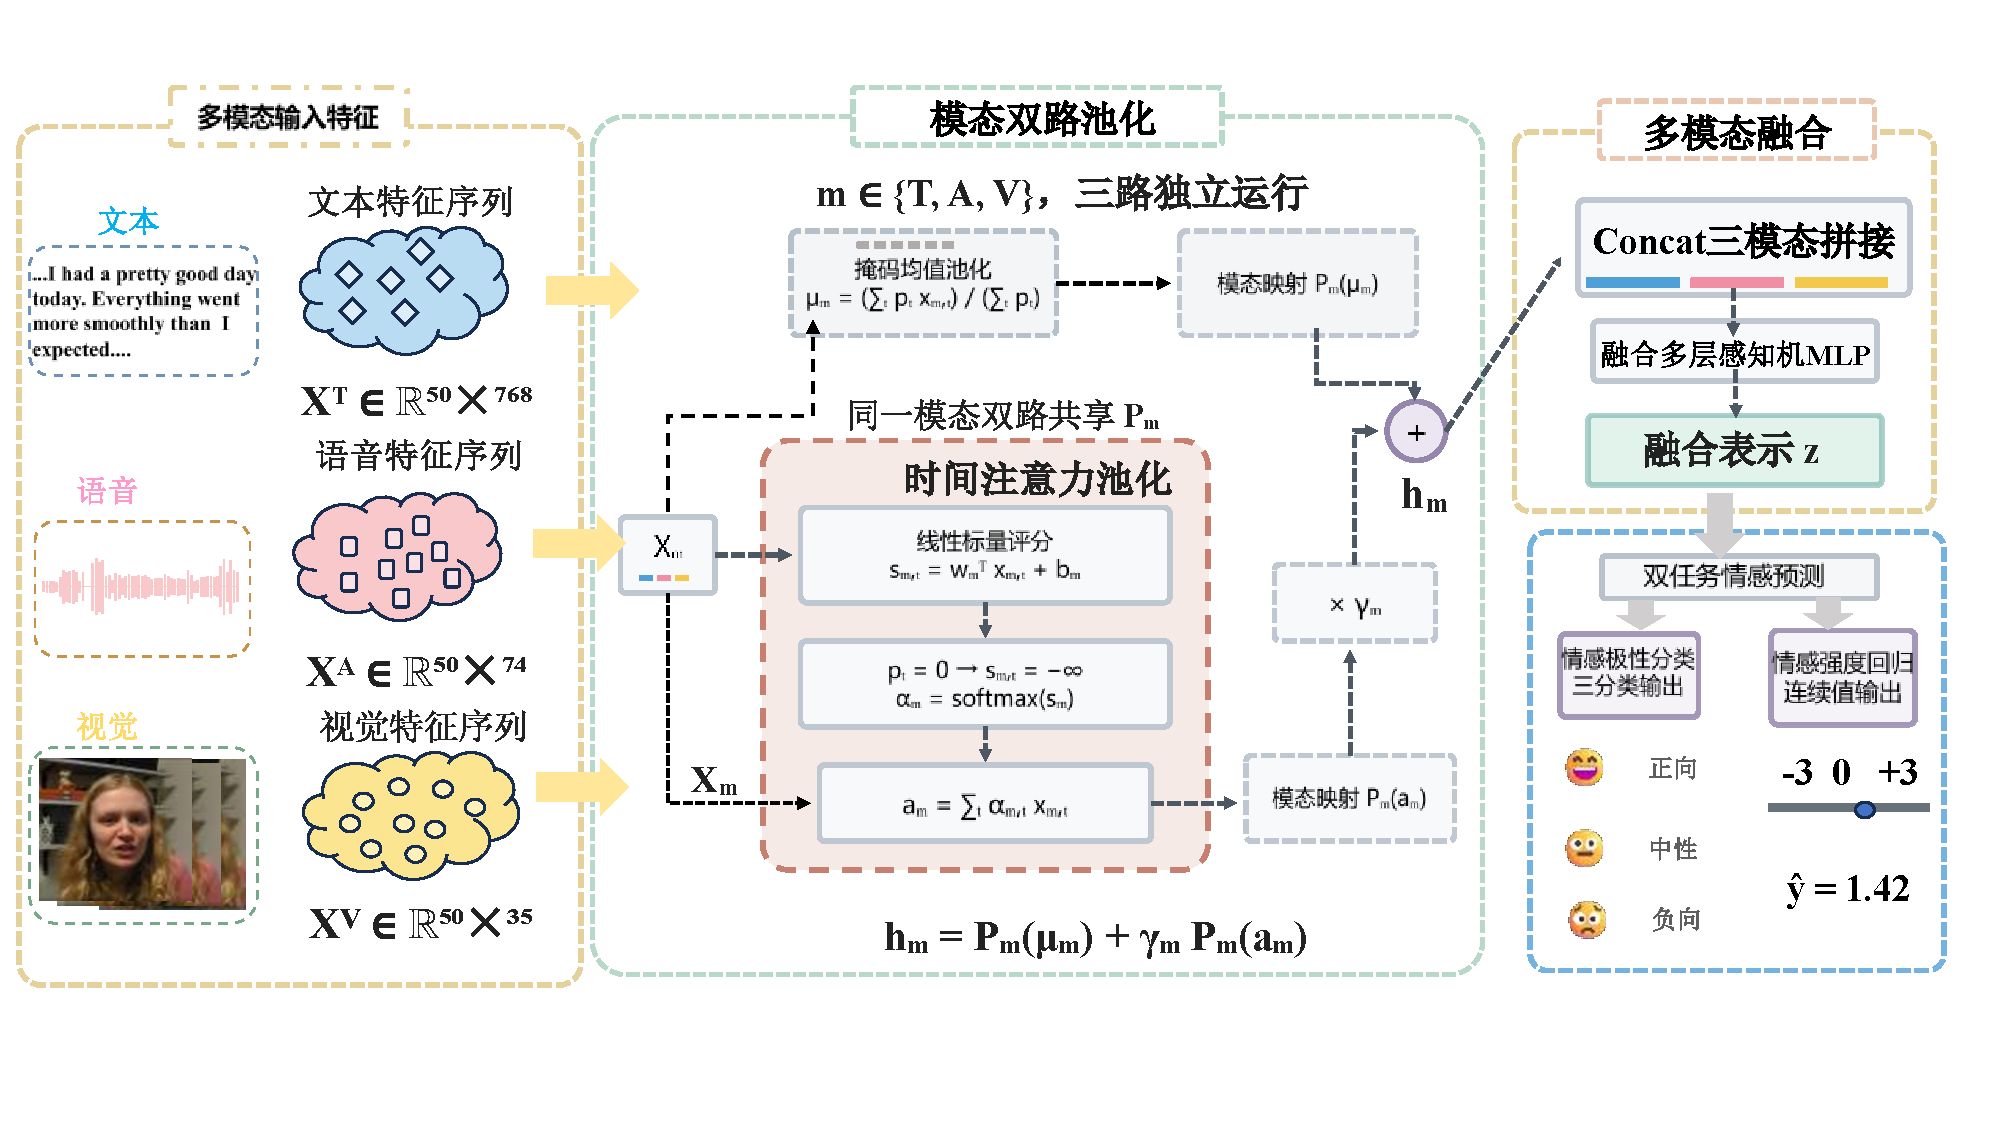
\includegraphics[width=.94\textwidth]{figures/q2/q2 架构图.pdf}
\caption{LTARP三模态池化与双任务预测流程。}
\label{fig:q2_arch}\end{figure}

\subsection{数据表示与预测任务}\label{subsec:q2_data}
\QTwoParagraph 为使后续比较主要反映聚合方式与缺失场景带来的差异，本文在统一的数据划分和标签定义下使用附件2的对齐输入。对齐特征文件为\texttt{aligned-50.pkl}，训练、验证和测试划分分别含3395、728和727条样本。训练集用于学习参数，验证集用于结构选择与评价；测试划分和无标签附件3不参与选模。

\QTwoParagraph 统一最大长度为$T=50$，样本$i$的三模态输入为
\begin{equation}
\mathbf X_i^{(T)} \in \mathbb R^{50 \times 768},\quad
\mathbf X_i^{(A)} \in \mathbb R^{50 \times 74},\quad
\mathbf X_i^{(V)} \in \mathbb R^{50 \times 35}.
\label{eq:q2_tensor_dim}
\end{equation}
样本有效长度为$L_i$（$3\le L_i\le50$），由随附注意力掩码确定。定义有效槽位指示变量
\begin{equation}
p_{it} = \begin{cases}
1, & t \in \{1, 2, \dots, L_i\},\\
0, & t \in \{L_i+1, \dots, 50\}.
\end{cases}
\label{eq:q2_mask_def}
\end{equation}
\QTwoParagraph 缺失实验仅作用于原本有效的时间位置。附件2中已有的零值输入保持原始状态，并与后续人为构造的连续缺失分别记录。填充后缀由掩码排除，原始有效范围在遮挡前后保持一致。人工置零的位置仍位于有效前缀中，均值聚合的分母继续使用原有效长度，模型因而接收相同长度、局部内容受损的序列。

\QTwoParagraph 连续情感强度标签记为$y_i\in[-3.0,+3.0]$，三类极性由其符号确定：
\begin{equation}
c_i = \begin{cases}
0 \quad (\text{消极 Negative}), & y_i < 0,\\
1 \quad (\text{中性 Neutral}), & y_i = 0,\\
2 \quad (\text{积极 Positive}), & y_i > 0.
\end{cases}
\label{eq:q2_label_split}
\end{equation}
其中$y_i=0$对应中性类，分类与回归分别描述极性类别和连续情感强度。

\QTwoParagraph 训练集与验证集均以积极样本为最多，中性样本相对较少，类别比例呈现不均衡；连续情感强度集中于零附近，两侧分布覆盖不同程度的极性。有效序列长度也有明显差异，训练与验证的中位数分别为22和23.5，小于统一长度50。因此，类别权重和有效位掩码分别进入损失计算与特征聚合（图~\ref{fig:q2_data}）。

\begin{figure}[htbp]\centering
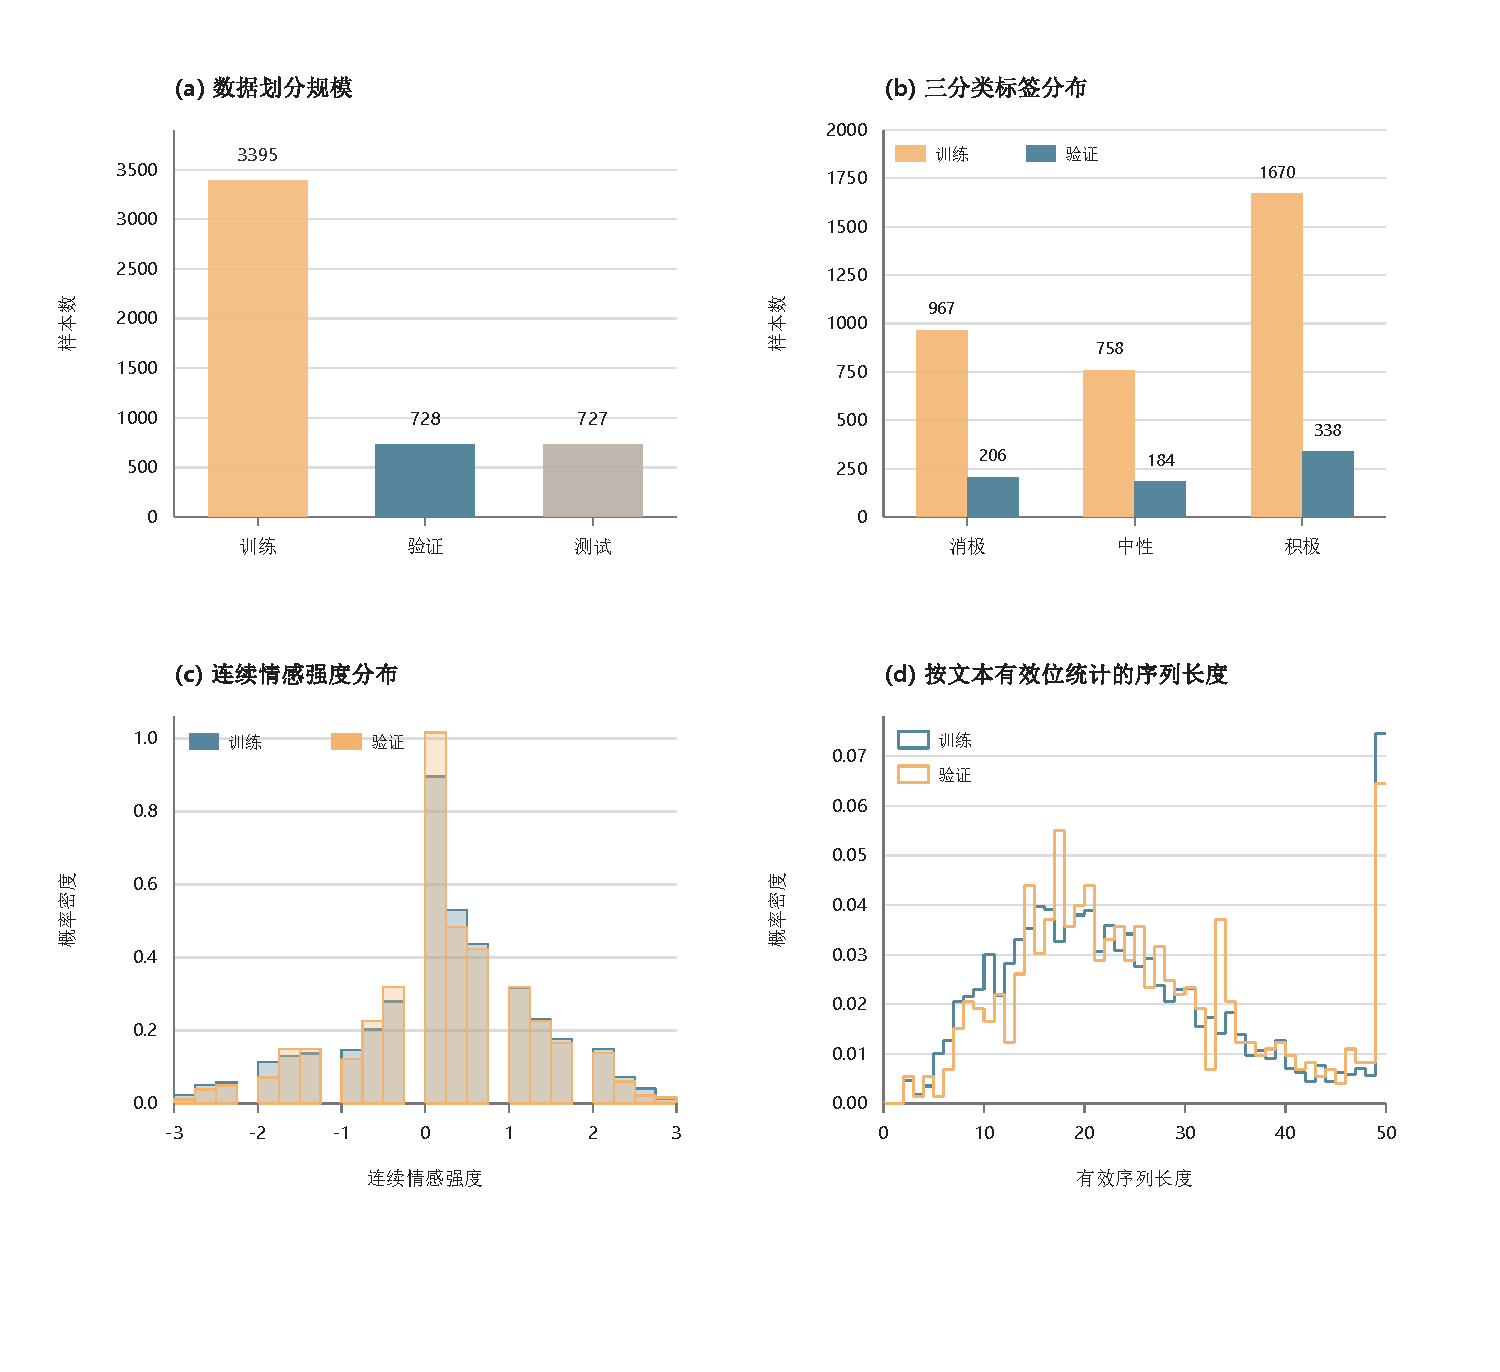
\includegraphics[width=.96\textwidth]{figures/q2/fig10_q2_data_statistics.pdf}
\caption{附件2的样本、情感标签与有效序列长度分布。}
\label{fig:q2_data}\end{figure}

\subsection{掩码均值池化基线}\label{subsec:q2_base}
\QTwoParagraph 在上述输入与任务定义基础上，本文首先建立掩码均值池化基线MMP，作为后续改进结构的比较参照。有效位掩码使填充后缀不参与聚合，各模态由此得到固定维度的均值向量，再接入共同的融合与双任务输出路径。对模态$m\in\{T,A,V\}$，其均值为
\begin{equation}
\boldsymbol\mu_i^{(m)} = \frac{\sum_{t=1}^{50} p_{it} \mathbf x_{it}^{(m)}}{\sum_{t=1}^{50} p_{it}}.
\label{eq:q2_mean_pool}
\end{equation}
均值向量通过模态专属映射$P_m(\cdot)$得到128维表示：
\begin{equation}
\mathbf h_{i,0}^{(m)} = P_m\left(\boldsymbol\mu_i^{(m)}\right) = \operatorname{Dropout}\Big(\operatorname{GELU}\big(\operatorname{LayerNorm}(\mathbf W_m \boldsymbol\mu_i^{(m)} + \mathbf b_m)\big)\Big).
\label{eq:q2_proj_layer}
\end{equation}
三路表示拼接为384维向量$\mathbf h_i^{\mathrm{concat}}=[\mathbf h_{i,0}^{(T)};\mathbf h_{i,0}^{(A)};\mathbf h_{i,0}^{(V)}]$，再经128维融合层得到
\begin{equation}
\mathbf z_i = \operatorname{Dropout}\Big(\operatorname{GELU}\big(\operatorname{LayerNorm}(\mathbf W_f \mathbf h_i^{\mathrm{concat}} + \mathbf b_f)\big)\Big).
\end{equation}
联合表征分别连接三分类与强度回归输出：
\begin{equation}
\hat{\mathbf p}_i = \operatorname{Softmax}(\mathbf W_c \mathbf z_i + \mathbf b_c) \in \mathbb R^3,\qquad
\hat y_i = \mathbf W_r \mathbf z_i + b_r \in \mathbb R.
\label{eq:q2_heads}
\end{equation}
预测类别取$\hat c_i=\arg\max_{k\in\{0,1,2\}}\hat p_{ik}$。

\QTwoParagraph 训练集的消极、中性和积极样本数分别为967、758和1670。采用类别频数逆加权交叉熵，使三类在分类目标中获得相应权重：
\begin{equation}
w_c = \frac{N_{\mathrm{train}}}{3 \cdot N_c},\qquad
\mathcal L_{\mathrm{WCE}} = -\frac{\sum_{i=1}^N w_{c_i}\log\hat p_{i c_i}}{\sum_{i=1}^N w_{c_i}}.
\end{equation}
其中分类损失按当前批次标签权重之和归一化，$N$为批次样本数。回归采用SmoothL1损失：
\begin{equation}
\mathcal L_{\mathrm{SmoothL1}} = \frac{1}{N}\sum_{i=1}^N \ell_{\mathrm{smooth}}(\hat y_i - y_i),\quad
\ell_{\mathrm{smooth}}(u) = \begin{cases}
0.5 u^2, & |u| < 1,\\
|u| - 0.5, & |u| \ge 1.
\end{cases}
\end{equation}
两项任务以相同权重联合优化：
\begin{equation}
\mathcal L = \mathcal L_{\mathrm{WCE}} + \lambda_r \mathcal L_{\mathrm{SmoothL1}},\qquad \lambda_r = 1.0.
\label{eq:q2_loss_full}
\end{equation}

\QTwoParagraph MMP共含163460个参数，直接使用附件2的原始数值特征，不额外标准化。采用AdamW，学习率$10^{-3}$、权重衰减$10^{-4}$、批量大小128、随机失活率0.1；最多训练80轮，提前停止耐心轮数为12轮。基线在完整输入上训练。

\subsection{轻量时间注意力残差池化模型}\label{subsec:q2_pool}
\QTwoParagraph 当局部连续缺失移除一段信息后，剩余有效位置所包含的情感信息并不均等。MMP仍采用等权聚合，难以突出更有判别力的位置。为使聚合权重能够随当前样本内容变化，LTARP在均值分支之外增加逐槽位内容打分，并将加权表示作为残差补充。每个模态使用一个线性标量打分器，其打分记为
\begin{equation}
e_{it}^{(m)} = f_m(\mathbf x_{it}^{(m)}) = \mathbf w_m^\top\mathbf x_{it}^{(m)} + b_m.
\end{equation}
权重在原始有效槽位内归一化，并形成内容加权表示：
\begin{equation}
\alpha_{it}^{(m)} = \frac{p_{it}\exp(e_{it}^{(m)})}{\sum_{s: p_{is}=1} \exp(e_{is}^{(m)})},\qquad
\mathbf a_i^{(m)} = \sum_{t=1}^{50} \alpha_{it}^{(m)} \mathbf x_{it}^{(m)}.
\label{eq:q2_alpha_softmax}
\end{equation}
填充位的$\alpha_{it}^{(m)}$恒为0。人工遮挡后的零值仍按原有效指示参与打分与聚合，权重变化由当前输入内容决定。

\QTwoParagraph 内容加权表示作为均值表示的补充，两路共享模态映射$P_m$，以可学习系数$\gamma_m$进行残差组合：
\begin{equation}
\mathbf h_i^{(m)} = P_m\big(\boldsymbol\mu_i^{(m)}\big) + \gamma_m \cdot P_m\big(\mathbf a_i^{(m)}\big), \quad m \in \{T, A, V\}.
\label{eq:q2_residual_composite}
\end{equation}
该表示继续进入原有融合层与双任务输出，新增分支只改变模态内的聚合方式。共享映射使两路表示具有相同维度，均值路径保留整体信息，内容加权路径提供随样本变化的补充；残差系数控制补充分支进入预测的程度。

\QTwoParagraph 训练首先完成MMP的模态映射、融合与双任务输出学习，再以其参数初始化LTARP。第二阶段保持这些已有参数不变，仅学习三个模态打分器及三个残差系数。令$\gamma_m$初值为0，初始模态输出为
\begin{equation}
\mathbf h_i^{(m)} = P_m(\boldsymbol\mu_i^{(m)}),
\end{equation}
与MMP保持一致。随后，内容加权分支通过残差系数逐步参与预测。新增可训练参数为883个，总参数量增至164343，从而以较小的参数增量补充时间位置的内容差异。

\subsection{连续缺失场景与评价协议}\label{subsec:q2_benchmark}
\QTwoParagraph 为系统比较不同连续缺失形式对预测的影响，并在相同受损条件下观察MMP与LTARP的表现，本文从缺失模态、缺失比例和缺失位置三个维度构造固定场景。单模态场景沿比例变化考察各输入的敏感程度，双模态场景在同一比例下考察信息同时受损的影响；前段、中段和后段遮挡则用于区分缺失发生位置。三个维度组合形成54种场景，使模型比较与缺失规律分析共享同一组受损输入。

\begin{itemize}[leftmargin=2.5em,itemsep=0pt,topsep=2pt]
\item 单模态场景集$\mathcal C_1$：$m\in\{T,A,V\}$，目标缺失比例$\rho_{\mathrm{target}}\in\mathcal R=\{0.1,0.2,0.3,0.4,0.5\}$，位置$\mathcal P=\{\text{前段},\text{中段},\text{后段}\}$，共$3\times5\times3=45$种。
\item 双模态场景集$\mathcal C_2$：模态对为$\{T,A\}$、$\{T,V\}$、$\{A,V\}$，固定$\rho_{\mathrm{target}}=0.3$，分别取三个位置，共$3\times1\times3=9$种。
\end{itemize}

\QTwoParagraph 对有效长度$L_i$，遮挡槽位数与实际比例为
\begin{equation}
\ell_i = \max\big(1,\, \operatorname{round}(\rho_{\mathrm{target}} \cdot L_i)\big),\qquad
\rho_{\mathrm{actual}, i} = \frac{\ell_i}{L_i}.
\label{eq:q2_mask_len}
\end{equation}
槽位数必须取整数，短序列的实际比例会偏离目标比例；验证集中，目标比例0.1的实际范围为0.0714--0.3333，目标比例0.5为0.4000--0.6667，对应均值为0.1040和0.5009。图表横轴用目标比例标识场景，实际比例逐样本记录。

\QTwoParagraph 前段、中段、后段的起点$s_i$分别为$0$、$\lfloor(L_i-\ell_i)/2\rfloor$和$L_i-\ell_i$。遮挡将指定模态在$[s_i,s_i+\ell_i-1]$内的特征置零，该遮挡区间采用零起始槽位索引；其余模态和填充掩码保持原样。每个场景都在完整的728条验证样本上评价，各样本按自身有效长度计算区间。

\QTwoParagraph 分类评价采用准确率和宏平均F1，分别观察总体识别结果和三类样本的均衡表现。
\begin{equation*}
\operatorname{Acc} = \frac{1}{N}\sum_{i=1}^N \mathbb I(\hat c_i = c_i).
\end{equation*}
\begin{equation*}
\operatorname{MacroF1} = \frac{1}{3}\sum_{k=0}^2 \frac{2 \cdot \operatorname{Precision}_k \cdot \operatorname{Recall}_k}{\operatorname{Precision}_k + \operatorname{Recall}_k}.
\end{equation*}
\QTwoParagraph 回归评价采用平均绝对误差和皮尔逊相关系数，分别反映连续强度的绝对偏差和预测趋势的一致程度。
\begin{equation*}
\operatorname{MAE} = \frac{1}{N}\sum_{i=1}^N |\hat y_i - y_i|.
\end{equation*}
\begin{equation*}
\operatorname{Pearson} = \frac{\sum_{i=1}^N (\hat y_i - \bar{\hat y})(y_i - \bar y)}{\sqrt{\sum_{i=1}^N (\hat y_i - \bar{\hat y})^2}\sqrt{\sum_{i=1}^N (y_i - \bar y)^2}}.
\end{equation*}

\QTwoParagraph 分类与回归分别反映极性识别和连续情感强度预测，单项指标不能同时概括两项任务。为在参数选择时兼顾二者，本文将四项评价指标组合为得分$S$：
\begin{equation}
S = \frac{1}{4}\operatorname{Acc} + \frac{1}{4}\operatorname{MacroF1} + \frac{1}{4}\left(1 - \frac{\operatorname{MAE}}{6}\right) + \frac{1}{8}(\operatorname{Pearson} + 1).
\label{eq:q2_score_s}
\end{equation}
连续情感强度标签位于$[-3,3]$，跨度为6，因此以$\operatorname{MAE}/6$缩放误差量级，并通过$1-\operatorname{MAE}/6$统一为越大越好的方向。Pearson的取值范围为$[-1,1]$，$(\operatorname{Pearson}+1)/2$将其映射至$[0,1]$，故式~\eqref{eq:q2_score_s}中的最后一项等价于给该映射值赋予$1/4$权重。两项分类指标合计占$1/2$，两项回归指标合计占$1/2$，兼顾极性识别与连续情感强度预测。回归输出不作截断，6作为标签尺度使用，而非预测误差的上界。

\QTwoParagraph 完整输入得分只能描述正常观测下的表现，连续缺失后的保持程度还需结合受损场景评价。本文将完整输入对应的得分记为$S_{\mathrm{clean}}$，并以其与54种缺失场景的平均得分共同定义综合鲁棒得分$R$：
\begin{equation}
R = \frac{1}{2}\left(S_{\mathrm{clean}} + \frac{1}{54}\sum_{j=1}^{54} S_j\right).
\label{eq:q2_robust_r}
\end{equation}
完整输入得分占$1/2$，54种缺失场景的等权平均占$1/2$。这一组合同时考虑正常输入与受损输入下的表现，使配置选择兼顾完整输入能力和缺失后的保持程度。

\QTwoParagraph 结构比较表~\ref{tab:q2_main}以及公开方法表~\ref{tab:q2_public_baselines}、\ref{tab:q2_public_missing}，均按完整输入验证得分$S_{\mathrm{clean}}$选择参数；选定后同时评价完整输入与全部54种缺失场景，保证两张公开方法结果表使用同一套参数。缺失敏感性与鲁棒诊断图~\ref{fig:q2_ratio}--\ref{fig:q2_error}则沿用按$R$选定的LTARP配置，MMP仍使用对应初始化的完整输入最优基线。前者比较统一完整输入标准下的结构表现，后者分析最终配置在固定缺失场景集合中的响应与波动；在每类实验内，每次初始化均固定一套参数，不按缺失模态、比例或位置重新选择。

\QTwoParagraph 场景统计先在种子内汇总，再计算种子间均值与样本标准差。设第$s$个种子在场景$j$的指标为$M_{s,j}$，其缺失场景均值为
\begin{equation}
\bar M_s = \frac{1}{54}\sum_{j=1}^{54}M_{s,j}, \qquad s\in\{42,43,44\}.
\end{equation}
三次初始化是统计重复单位，54个场景在各自初始化内等权平均。这样，场景平均表示模型在固定受损条件集合中的总体表现，种子间标准差则描述同一训练设置的初始化波动。算法~\ref{alg:q2_benchmark}概括执行步骤。

\begin{table}[htbp]
\centering\zihao{-4}
\refstepcounter{q2algorithm}\label{alg:q2_benchmark}
算法\arabic{q2algorithm}\quad 连续缺失场景评价\par
\vspace{0.5em}
\renewcommand{\arraystretch}{1.15}
\begin{tabularx}{\textwidth}{@{}>{\raggedright\arraybackslash}X@{}}
\toprule
\textbf{输入}：验证集三模态特征、有效掩码与已选模型。\\
\textbf{输出}：完整输入及54场景指标、$S_{\mathrm{clean}}$与$R$。\\
\midrule
1. 预测完整输入，计算四项指标及$S_{\mathrm{clean}}$。\\
2. 遍历场景配置$(\mathcal M_{\mathrm{target}},\rho_{\mathrm{target}},\mathrm{pos})$。\\
3. 对各样本读取$L_i$，按式~\eqref{eq:q2_mask_len}计算$\ell_i$并确定$s_i$。\\
4. 在原输入副本中置零目标模态的连续区间，保持有效掩码。\\
5. 预测当前场景，记录四项指标与$S_j$。\\
6. 汇总54场景结果，按式~\eqref{eq:q2_robust_r}计算$R$。\\
\bottomrule
\end{tabularx}
\end{table}
\FloatBarrier

\subsection{基线与LTARP的结构比较}\label{subsec:q2_fair}
\QTwoParagraph 首先在统一完整输入选模标准下直接比较MMP与LTARP，以观察聚合结构改变后的分类与回归表现。LTARP在宏平均 F1、MAE和Pearson的三种子均值上均优于MMP，准确率变化较小。对相同模型参数施加54种缺失后，三项指标的平均改善仍保留，准确率则略有下降（表~\ref{tab:q2_main}）。MAE与Pearson的改善分别对应连续情感强度绝对误差的减少和预测趋势的一致性提高。

\QTwoParagraph 验证集中积极样本最多，准确率按样本汇总，受多数类别识别情况的影响较大；宏平均 F1对三类等权，能够反映整体准确率之外的类别差异。当前改善更多体现在宏平均 F1，说明评价两种池化结构时需要同时观察总体识别和类别均衡表现。中性类的混淆仍然明显，其具体错误分布在后续分析中结合混淆矩阵观察。

\begin{table}[H]
\centering\zihao{-4}\setlength{\tabcolsep}{4pt}
\caption{统一完整输入选模规则下的MMP与LTARP比较（三随机种子均值$\pm$样本标准差）}
\label{tab:q2_main}
\begin{tabularx}{\textwidth}{@{}>{\raggedright\arraybackslash}p{2.5cm}l*{4}{>{\centering\arraybackslash}X}@{}}
\toprule
条件 & 模型 & 准确率$\uparrow$ & 宏平均F1$\uparrow$ & MAE$\downarrow$ & 相关系数$\uparrow$\\
\midrule
完整输入 & MMP & \shortstack{$0.6401$\\$\pm0.0048$} & \shortstack{$0.6139$\\$\pm0.0091$} & \shortstack{$0.6079$\\$\pm0.0103$} & \shortstack{$0.6409$\\$\pm0.0043$}\\
完整输入 & LTARP & \shortstack{$0.6415$\\$\pm0.0050$} & \shortstack{$0.6243$\\$\pm0.0026$} & \shortstack{$0.6052$\\$\pm0.0063$} & \shortstack{$0.6475$\\$\pm0.0024$}\\
\addlinespace
54场景平均 & MMP & \shortstack{$0.6349$\\$\pm0.0062$} & \shortstack{$0.6092$\\$\pm0.0075$} & \shortstack{$0.6111$\\$\pm0.0098$} & \shortstack{$0.6359$\\$\pm0.0038$}\\
54场景平均 & LTARP & \shortstack{$0.6334$\\$\pm0.0038$} & \shortstack{$0.6163$\\$\pm0.0013$} & \shortstack{$0.6086$\\$\pm0.0059$} & \shortstack{$0.6417$\\$\pm0.0024$}\\
\bottomrule
\end{tabularx}
\end{table}

\QTwoParagraph 为观察随机初始化对跨场景表现的影响，进一步比较三个随机种子的综合得分。种子42和43呈正增益，种子44近乎持平；配对差$\Delta R=R_{\mathrm{LTARP}}-R_{\mathrm{MMP}}$分别为$+0.005600$、$+0.003791$和$-0.000090$，平均为$+0.003100\pm0.002907$。总体收益较小，同时存在初始化敏感性。
\FloatBarrier

\subsection{缺失类型、位置与比例分析}\label{subsec:q2_patterns}
\QTwoParagraph 表~\ref{tab:q2_main}给出了完整输入与54种缺失场景的总体平均，但平均值不能呈现不同缺失模态、比例和位置的差异。为进一步辨别这些差异，以下分解考察最终鲁棒配置的缺失响应。图~\ref{fig:q2_ratio}首先反映缺失比例的影响：文本随遮挡比例增大呈现最明显的持续退化，语音和视觉曲线则相对平缓。文本遮挡由0.1增至0.5时，宏平均 F1从0.6163降至0.5933，准确率也持续下降；相比之下，单独遮挡语音时两项分类指标基本保持，视觉缺失仅引起较小幅度的下降。在当前验证集与模型下，扩大文本缺失范围对分类结果的影响更突出。

\QTwoParagraph 分类与回归指标的变化节奏并不一致。文本缺失下，宏平均 F1在中等缺失比例附近变化较缓，而在较高比例时下降加快；Pearson随缺失比例增加持续降低，高比例缺失时降幅进一步扩大。MAE总体上升，但中间比例段存在轻微波动，并非与分类指标同步变化。这说明连续信息损失既可能改变类别判别，也可能改变强度预测的误差与相关性，四项指标对损失程度的响应不能相互替代。语音和视觉的回归曲线同样较平缓，与分类曲线中的模态差异相呼应。

\begin{figure}[htbp]\centering
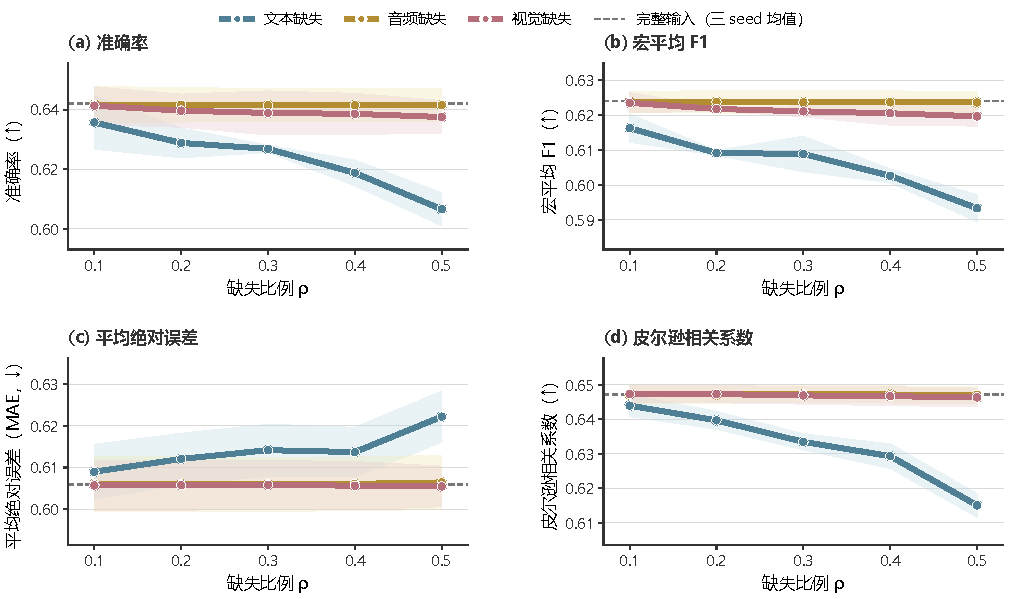
\includegraphics[width=.96\textwidth]{figures/q2/fig11_q2_modality_missing_degradation.pdf}
\caption{单模态缺失比例与验证集性能。阴影表示三次随机初始化的样本标准差，虚线表示完整输入均值。}
\label{fig:q2_ratio}\end{figure}
\FloatBarrier

\QTwoParagraph 固定目标缺失比例$\rho_{\mathrm{target}}=0.3$后，图~\ref{fig:q2_location}进一步区分缺失模态与缺失位置的作用。文本缺失造成的退化最明显，语音单独缺失的平均影响接近0，视觉缺失的影响则小于文本。文本前、中、后段遮挡对应的宏平均 F1变化约为$-0.018$、$-0.006$和$-0.021$，表明分类表现对前段和后段信息损失更敏感；Pearson变化约为$-0.024$、$-0.009$和$-0.009$，其损失主要集中在前段。文本中段遮挡虽使宏平均 F1下降，MAE却出现约$+0.003$的轻微改善；这里MAE变化按完整输入误差减缺失输入误差计，正值表示误差减小。分类与回归对缺失位置的响应不同，因此不能仅依据一项指标判断哪个位置的损失最大。

\QTwoParagraph 双模态缺失的变化模式进一步体现了这一差异。文本--语音与文本--视觉组合在分类和回归指标上的变化均与文本单模态缺失较为接近，语音--视觉组合则更接近视觉单模态缺失。联合缺失并未在各项指标上形成一致的叠加退化；在当前验证集与模型下，文本受损对主要退化方向的影响更突出。

\begin{figure}[htbp]\centering
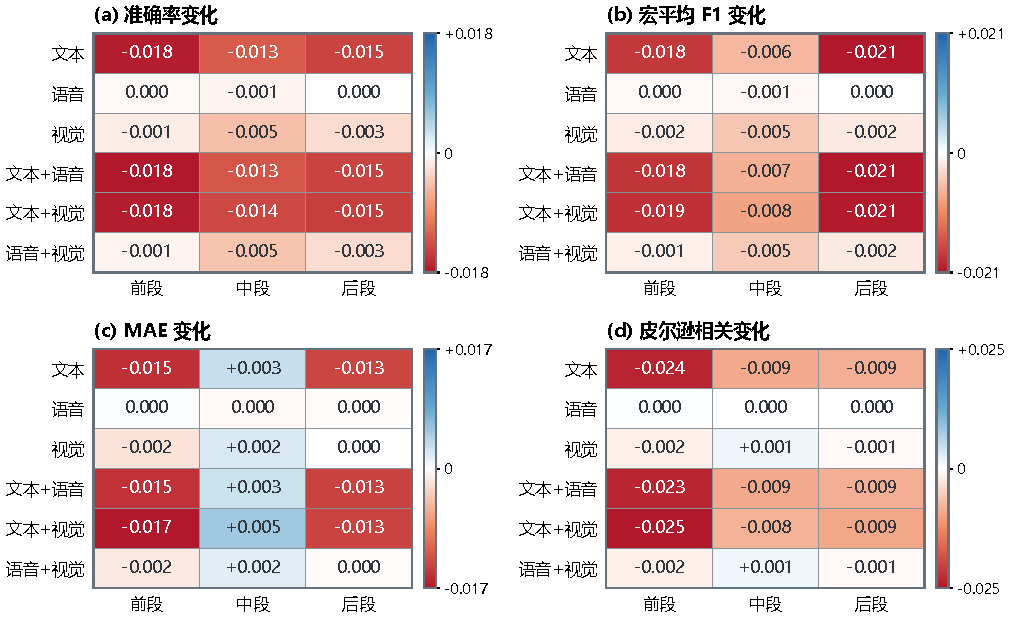
\includegraphics[width=.96\textwidth]{figures/q2/fig12_q2_modality_location_absolute_degradation.pdf}
\caption{不同模态与缺失位置相对完整输入的指标变化（目标缺失比例$\rho_{\mathrm{target}}=0.3$）。数值为三次随机初始化的配对均值，各指标使用独立色标；MAE采用“完整输入$-$缺失输入”，其余指标采用“缺失输入$-$完整输入”，因此正值均表示性能改善。}
\label{fig:q2_location}\end{figure}
\FloatBarrier

\QTwoParagraph 在比例与位置规律之外，图~\ref{fig:q2_gain}进一步比较最终鲁棒配置与MMP基线在相同受损场景下的响应差异。此处LTARP采用按$R$选定的配置，分析目的在于观察最终配置的场景收益；图中结果不是统一选模标准下的结构公平比较，直接结构比较仍以表~\ref{tab:q2_main}为准。宏平均 F1和Pearson在大多数场景中呈正增益，单独语音或视觉缺失时，三个位置的改善方向较一致；语音--视觉双模态缺失下，宏平均 F1也保持较稳定的正增益。在仍保留文本输入的这些场景中，LTARP相对MMP的收益较为一致。

\QTwoParagraph 文本缺失及包含文本的双模态缺失呈现另一种响应：准确率增量为负，宏平均 F1却仍常保持正增益，Pearson也大多改善。这表明LTARP的收益更多体现在类别均衡表现和连续情感预测，而非所有指标同步提高；MAE增益在部分位置接近0或略为负值，也体现了改进的场景边界。上述模式与表~\ref{tab:q2_main}中宏平均 F1、MAE和Pearson改善而准确率变化较小的结果相呼应，但两处比较采用的选模口径不同，不能据此将最终配置的全部收益归因于池化结构。图~\ref{fig:q2_gain}描述两种固定配置在不同受损输入下的指标差异，图~\ref{fig:q2_location}则描述缺失输入相对完整输入的性能变化，两者分别用于观察配置响应和信息损失规律。

\begin{figure}[htbp]\centering
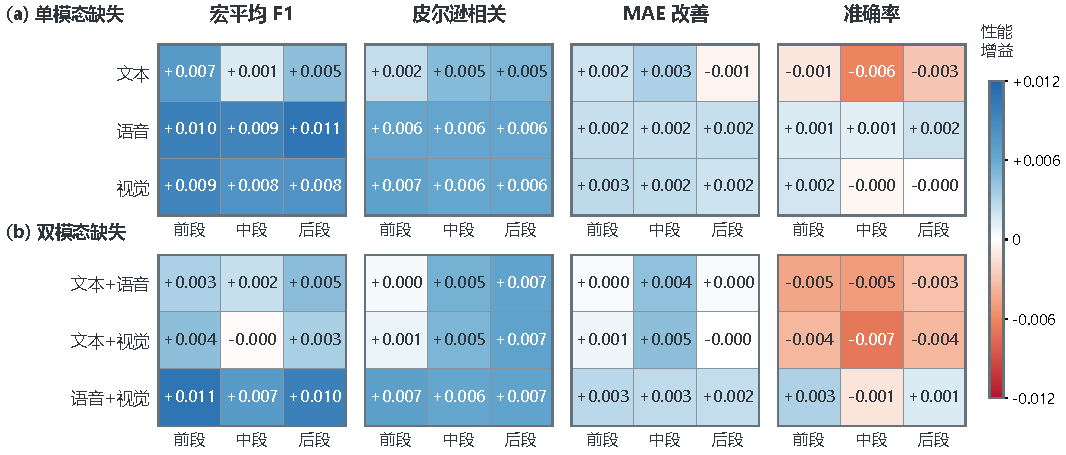
\includegraphics[width=.96\textwidth]{figures/q2/fig13_q2_p2_minus_b0_modality_location_gain.pdf}
\caption{最终鲁棒配置与MMP基线在不同缺失场景下的指标差异。数值为三次随机初始化的均值差；MAE取MMP$-$LTARP，其余指标取LTARP$-$MMP，因此正值均表示LTARP对应指标更优。}
\label{fig:q2_gain}\end{figure}
\FloatBarrier

\subsection{稳定性、错误分布与消融分析}\label{subsec:q2_ablation}
\subsubsection{随机初始化稳定性与验证集错误分布}
\QTwoParagraph 前述分析给出了不同缺失场景的平均响应，下面进一步从随机初始化、类别混淆和特殊输入三个方面观察这些结果的保持程度。三次初始化的配对收益较小，结合完整输入分类错误与原生视觉全零样本，可以识别总体平均之外的差异（图~\ref{fig:q2_error}）。

\begin{figure}[H]\centering
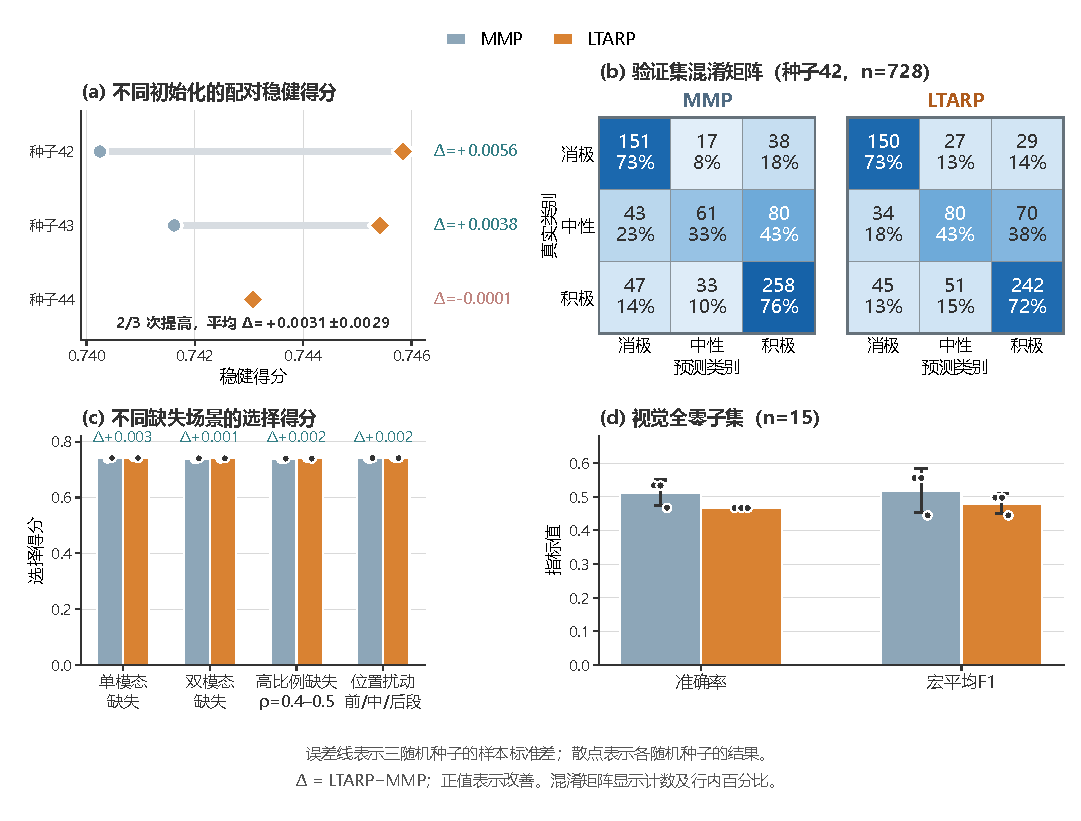
\includegraphics[width=.96\textwidth]{figures/q2/fig14_q2_stability_error_analysis.pdf}
\caption{随机初始化稳定性与误差分析。（a）配对综合分数；（b）混淆矩阵；（c）场景分组；（d）原生视觉全零子集。}
\label{fig:q2_error}\end{figure}
\FloatBarrier

\QTwoParagraph 三次初始化中有两次提高，一次近乎持平，场景分组后的平均差也较小。完整输入下，消极与积极类的召回相对较高，中性类最低，为43.48\%；中性样本更容易被分到两侧极性类别，弱极性与类别边界仍是主要混淆位置。

\QTwoParagraph 验证集另有15条原生视觉特征整段全零样本。该子集中，部分初始化的LTARP分类表现低于MMP，呈现与总体平均趋势不同的结果；样本量较少，其表现结合三次初始化单独观察。

\subsubsection{候选结构与训练策略消融}
\QTwoParagraph 在考察最终配置的稳定性与错误分布后，进一步比较不同结构和训练调整能否带来类似收益。本文保留时间编码、训练期连续遮挡和均值--最大值残差池化三种候选，与MMP及LTARP并列（表~\ref{tab:q2_ablation}）。

\begin{table}[H]\centering\zihao{-4}
\caption{候选结构与训练策略消融。均值--最大值残差池化仅有一次初始化。}
\label{tab:q2_ablation}
\begin{tabular}{lccc}
\toprule
方案 & 初始化次数 & 总参数量 & 综合分数$R$\\
\midrule
MMP（基线） & 3 & 163460 & $0.7417\pm0.0015$\\
单模态时间编码 & 3 & 957572 & $0.7351\pm0.0020$\\
训练期连续遮挡 & 3 & 163460 & $0.7385\pm0.0025$\\
均值--最大值残差池化 & 1 & 163463 & $0.7443$\\
LTARP（本文方案） & 3 & 164343 & $0.7448\pm0.0015$\\
\bottomrule
\end{tabular}
\end{table}

\QTwoParagraph 单模态时间编码在聚合前加入顺序建模，参数量明显增加，综合得分却低于MMP。训练期连续遮挡保持网络不变：每条样本以0.5概率保留完整输入，其余样本中75\%遮挡一个模态、25\%遮挡两个模态，比例从$\{0.1,0.2,0.3,0.4,0.5\}$选择，起点在有效范围内随机确定，掩码保持原值。这种缺失增强也未带来综合得分改善。

\QTwoParagraph 均值--最大值残差池化沿用式~\eqref{eq:q2_mean_pool}的掩码均值表示，并增加有效槽位上的逐特征维最大值，再经残差组合接入原有网络。其得分接近LTARP，但仅保留一次初始化结果，主要作为结构探索参考，不与三随机种子结果作精细统计比较。LTARP的三种子综合均值在本组最高，同时只增加883个参数，在本组候选中提供了较好的综合表现。
\FloatBarrier

\subsection{公开方法适配与对比}\label{subsec:q2_public}
\QTwoParagraph 完成MMP与LTARP的内部比较及候选结构分析后，为考察LTARP与其他多模态建模路线的相对表现，本文进一步选取11种公开方法进行统一适配比较。各方法使用附件2的aligned-50输入与分类、回归双任务接口，三模态维度、数据划分、指标和完整输入选模标准保持一致，并按既有适配配置训练。表~\ref{tab:q2_public_overview}概括适配中的机制与规模。

\begin{table}[H]
\centering\zihao{-4}\setlength{\tabcolsep}{4pt}
\caption{公开方法的统一接口适配概览}\label{tab:q2_public_overview}
\begin{tabularx}{.98\textwidth}{@{}>{\raggedright\arraybackslash}p{.17\textwidth}>{\raggedright\arraybackslash}p{.15\textwidth}>{\raggedright\arraybackslash}X r@{}}
\toprule
方法 & 类型 & 本文适配中的核心机制 & 参数量\\
\midrule
TFN\cite{q2tfn} & 张量融合 & 三路表示增广后的外积融合 & 4,840,670\\
LMF\cite{q2lmf} & 低秩融合 & 模态专属低秩因子融合 & 323,276\\
MFN\cite{q2mfn} & 时序记忆融合 & 三路递归编码、记忆注意力与门控记忆 & 261,764\\
MulT\cite{q2mult} & 跨模态注意力 & 六路定向跨模态注意力与模态内记忆 & 624,094\\
MISA\cite{q2misa} & 表征解耦 & 共享/特有表示、重构与差异约束 & 1,118,852\\
Self-MM\cite{q2selfmm} & 多任务辅助学习 & 融合预测与单模态伪目标辅助监督 & 82,119\\
MMIM\cite{q2mmim} & 互信息约束 & 模态间及融合--单模态的InfoNCE约束 & 163,204\\
\addlinespace
TFR-Net\cite{q2tfr} & 缺失重构 & 连续遮挡、时序上下文与潜在表示重构 & 415,620\\
MissModal\cite{q2missmodal} & 缺失表征对齐 & 几何对比、分布与情感语义对齐 & 163,204\\
M3S\cite{q2m3s} & 缺失元采样 & 低秩骨干、完整支持/缺失查询的一步一阶元更新 & 323,276\\
MMIN\cite{q2mmin} & 缺失模态推断 & 潜在表示推断、残差细化与循环约束 & 292,164\\
\bottomrule
\end{tabularx}
\end{table}


\QTwoParagraph 这些方法分别通过张量交互、时序记忆、表征约束或辅助任务组织多模态信息，缺失增强方法还引入重构、表征对齐、元采样及潜在表示推断。比较同时考察完整输入预测能力、连续缺失后的表现和参数规模：前两项反映同一配置在不同输入条件下的结果，参数量补充表示模型复杂度。各方法接入统一特征与双任务接口，以下结果均限定在本文统一适配与评价设置下。

\QTwoParagraph 在本文统一适配与评价设置下，LTARP在完整输入的四项指标上均取得表~\ref{tab:q2_public_baselines}中最优的三随机种子均值。部分轻量方法及缺失增强方法的表现接近LTARP，而更复杂的融合结构未呈现同等的平均优势。Self-MM和MMIM借助辅助任务或信息约束，在较小规模下也保留了较强预测信息；TFR-Net的宏平均 F1接近LTARP，但回归指标有所差异。因此，分类均衡性和回归结果需要结合观察。

\begin{table}[H]
\centering\zihao{-4}\setlength{\tabcolsep}{2.25pt}
\caption{公开方法与LTARP的完整输入验证集结果（三随机种子均值$\pm$样本标准差）}
\label{tab:q2_public_baselines}
\begin{tabularx}{\textwidth}{@{}>{\raggedright\arraybackslash}p{2.0cm}>{\centering\arraybackslash}p{2.5cm}>{\centering\arraybackslash}p{2.1cm}*{4}{>{\centering\arraybackslash}X}@{}}
\toprule
模型 & 训练方式 & 参数量 & 准确率$\uparrow$ & \shortstack{宏平均\\F1$\uparrow$} & MAE$\downarrow$ & \shortstack{相关系数\\$\uparrow$}\\
\midrule
TFN & \shortstack{完整输入\\训练} & 4,840,670 & \shortstack{$0.6099$\\$\pm0.0076$} & \shortstack{$0.5872$\\$\pm0.0083$} & \shortstack{$0.6336$\\$\pm0.0102$} & \shortstack{$0.6056$\\$\pm0.0098$}\\
LMF & \shortstack{完整输入\\训练} & 323,276 & \shortstack{$0.5925$\\$\pm0.0114$} & \shortstack{$0.5719$\\$\pm0.0090$} & \shortstack{$0.6682$\\$\pm0.0196$} & \shortstack{$0.5807$\\$\pm0.0188$}\\
MFN & \shortstack{完整输入\\训练} & 261,764 & \shortstack{$0.5966$\\$\pm0.0080$} & \shortstack{$0.5824$\\$\pm0.0062$} & \shortstack{$0.6418$\\$\pm0.0124$} & \shortstack{$0.5908$\\$\pm0.0125$}\\
MulT & \shortstack{完整输入\\训练} & 624,094 & \shortstack{$0.6172$\\$\pm0.0148$} & \shortstack{$0.5891$\\$\pm0.0236$} & \shortstack{$0.6221$\\$\pm0.0260$} & \shortstack{$0.6369$\\$\pm0.0115$}\\
MISA & \shortstack{完整输入\\训练} & 1,118,852 & \shortstack{$0.6131$\\$\pm0.0083$} & \shortstack{$0.6010$\\$\pm0.0060$} & \shortstack{$0.9175$\\$\pm0.1005$} & \shortstack{$0.6269$\\$\pm0.0087$}\\
Self-MM & \shortstack{完整输入\\训练} & 82,119 & \shortstack{$0.6355$\\$\pm0.0052$} & \shortstack{$0.6107$\\$\pm0.0084$} & \shortstack{$0.6099$\\$\pm0.0066$} & \shortstack{$0.6423$\\$\pm0.0042$}\\
MMIM & \shortstack{完整输入\\训练} & 163,204 & \shortstack{$0.6360$\\$\pm0.0048$} & \shortstack{$0.6110$\\$\pm0.0007$} & \shortstack{$0.6102$\\$\pm0.0098$} & \shortstack{$0.6375$\\$\pm0.0054$}\\
\addlinespace\midrule
TFR-Net & \shortstack{缺失增强\\训练} & 415,620 & \shortstack{$0.6374$\\$\pm0.0071$} & \shortstack{$0.6230$\\$\pm0.0080$} & \shortstack{$0.6145$\\$\pm0.0118$} & \shortstack{$0.6267$\\$\pm0.0142$}\\
MissModal & \shortstack{缺失增强\\训练} & 163,204 & \shortstack{$0.6305$\\$\pm0.0071$} & \shortstack{$0.6108$\\$\pm0.0069$} & \shortstack{$0.6084$\\$\pm0.0113$} & \shortstack{$0.6431$\\$\pm0.0006$}\\
M3S & \shortstack{缺失增强\\训练} & 323,276 & \shortstack{$0.6035$\\$\pm0.0063$} & \shortstack{$0.5775$\\$\pm0.0169$} & \shortstack{$0.6706$\\$\pm0.0173$} & \shortstack{$0.5793$\\$\pm0.0171$}\\
MMIN & \shortstack{缺失增强\\训练} & 292,164 & \shortstack{$0.6383$\\$\pm0.0062$} & \shortstack{$0.6117$\\$\pm0.0079$} & \shortstack{$0.6279$\\$\pm0.0247$} & \shortstack{$0.6401$\\$\pm0.0027$}\\
\addlinespace\midrule
LTARP & \shortstack{完整输入\\训练} & 164,343 & \shortstack{$0.6415$\\$\pm0.0050$} & \shortstack{$0.6243$\\$\pm0.0026$} & \shortstack{$0.6052$\\$\pm0.0063$} & \shortstack{$0.6475$\\$\pm0.0024$}\\
\bottomrule
\end{tabularx}
\end{table}

\QTwoParagraph 在本文统一适配与评价设置下，54种连续缺失等权平均后，LTARP的宏平均 F1和Pearson在表~\ref{tab:q2_public_missing}中最高，MAE最低，准确率与TFR-Net、MMIN接近。完整输入表现与缺失后保持程度共同决定跨场景结果；缺失增强方法之间也存在差异。

\begin{table}[H]
\centering\zihao{-4}\setlength{\tabcolsep}{2.25pt}
\caption{公开方法与LTARP的54种连续缺失场景平均结果（三随机种子均值$\pm$样本标准差）}
\label{tab:q2_public_missing}
\begin{tabularx}{\textwidth}{@{}>{\raggedright\arraybackslash}p{2.0cm}>{\centering\arraybackslash}p{2.5cm}>{\centering\arraybackslash}p{2.1cm}*{4}{>{\centering\arraybackslash}X}@{}}
\toprule
模型 & 训练方式 & 参数量 & 准确率$\uparrow$ & \shortstack{宏平均\\F1$\uparrow$} & MAE$\downarrow$ & \shortstack{相关系数\\$\uparrow$}\\
\midrule
TFN & \shortstack{完整输入\\训练} & 4,840,670 & \shortstack{$0.5767$\\$\pm0.0197$} & \shortstack{$0.5582$\\$\pm0.0127$} & \shortstack{$0.6451$\\$\pm0.0101$} & \shortstack{$0.5784$\\$\pm0.0070$}\\
LMF & \shortstack{完整输入\\训练} & 323,276 & \shortstack{$0.5616$\\$\pm0.0054$} & \shortstack{$0.5392$\\$\pm0.0066$} & \shortstack{$0.6630$\\$\pm0.0123$} & \shortstack{$0.5539$\\$\pm0.0185$}\\
MFN & \shortstack{完整输入\\训练} & 261,764 & \shortstack{$0.5657$\\$\pm0.0070$} & \shortstack{$0.5532$\\$\pm0.0081$} & \shortstack{$0.6559$\\$\pm0.0097$} & \shortstack{$0.5540$\\$\pm0.0092$}\\
MulT & \shortstack{完整输入\\训练} & 624,094 & \shortstack{$0.6000$\\$\pm0.0209$} & \shortstack{$0.5749$\\$\pm0.0230$} & \shortstack{$0.6309$\\$\pm0.0189$} & \shortstack{$0.6232$\\$\pm0.0057$}\\
MISA & \shortstack{完整输入\\训练} & 1,118,852 & \shortstack{$0.6079$\\$\pm0.0095$} & \shortstack{$0.5958$\\$\pm0.0080$} & \shortstack{$0.9247$\\$\pm0.1025$} & \shortstack{$0.6198$\\$\pm0.0077$}\\
Self-MM & \shortstack{完整输入\\训练} & 82,119 & \shortstack{$0.6302$\\$\pm0.0016$} & \shortstack{$0.6053$\\$\pm0.0042$} & \shortstack{$0.6131$\\$\pm0.0068$} & \shortstack{$0.6371$\\$\pm0.0040$}\\
MMIM & \shortstack{完整输入\\训练} & 163,204 & \shortstack{$0.6302$\\$\pm0.0041$} & \shortstack{$0.6059$\\$\pm0.0004$} & \shortstack{$0.6135$\\$\pm0.0101$} & \shortstack{$0.6332$\\$\pm0.0051$}\\
\addlinespace\midrule
TFR-Net & \shortstack{缺失增强\\训练} & 415,620 & \shortstack{$0.6336$\\$\pm0.0099$} & \shortstack{$0.6154$\\$\pm0.0098$} & \shortstack{$0.6232$\\$\pm0.0146$} & \shortstack{$0.6220$\\$\pm0.0143$}\\
MissModal & \shortstack{缺失增强\\训练} & 163,204 & \shortstack{$0.6260$\\$\pm0.0096$} & \shortstack{$0.6068$\\$\pm0.0048$} & \shortstack{$0.6111$\\$\pm0.0112$} & \shortstack{$0.6381$\\$\pm0.0013$}\\
M3S & \shortstack{缺失增强\\训练} & 323,276 & \shortstack{$0.5733$\\$\pm0.0056$} & \shortstack{$0.5493$\\$\pm0.0102$} & \shortstack{$0.6620$\\$\pm0.0071$} & \shortstack{$0.5581$\\$\pm0.0192$}\\
MMIN & \shortstack{缺失增强\\训练} & 292,164 & \shortstack{$0.6341$\\$\pm0.0049$} & \shortstack{$0.6072$\\$\pm0.0039$} & \shortstack{$0.6318$\\$\pm0.0259$} & \shortstack{$0.6346$\\$\pm0.0037$}\\
\addlinespace\midrule
LTARP & \shortstack{完整输入\\训练} & 164,343 & \shortstack{$0.6334$\\$\pm0.0038$} & \shortstack{$0.6163$\\$\pm0.0013$} & \shortstack{$0.6086$\\$\pm0.0059$} & \shortstack{$0.6417$\\$\pm0.0024$}\\
\bottomrule
\end{tabularx}
\end{table}
\FloatBarrier

\QTwoParagraph 在上述性能结果基础上，再结合参数量比较各方法的模型规模。LTARP总参数量为164343，约16.4万，明显小于TFN、MulT和MISA等结构，与MMIM和MissModal处于相近量级。在表~\ref{tab:q2_public_baselines}--\ref{tab:q2_public_missing}所列模型中，其完整输入和缺失平均宏平均 F1均保持较高水平。图~\ref{fig:q2_params}分别对照这两类输入条件；不同方法的参数规模跨越一个数量级以上，横轴采用对数尺度，使轻量结构和较大融合网络能够在同一坐标中比较。这组结果体现了LTARP在当前接口下的性能与规模平衡，结构复杂度本身不足以决定预测表现。

\begin{figure}[htbp]\centering
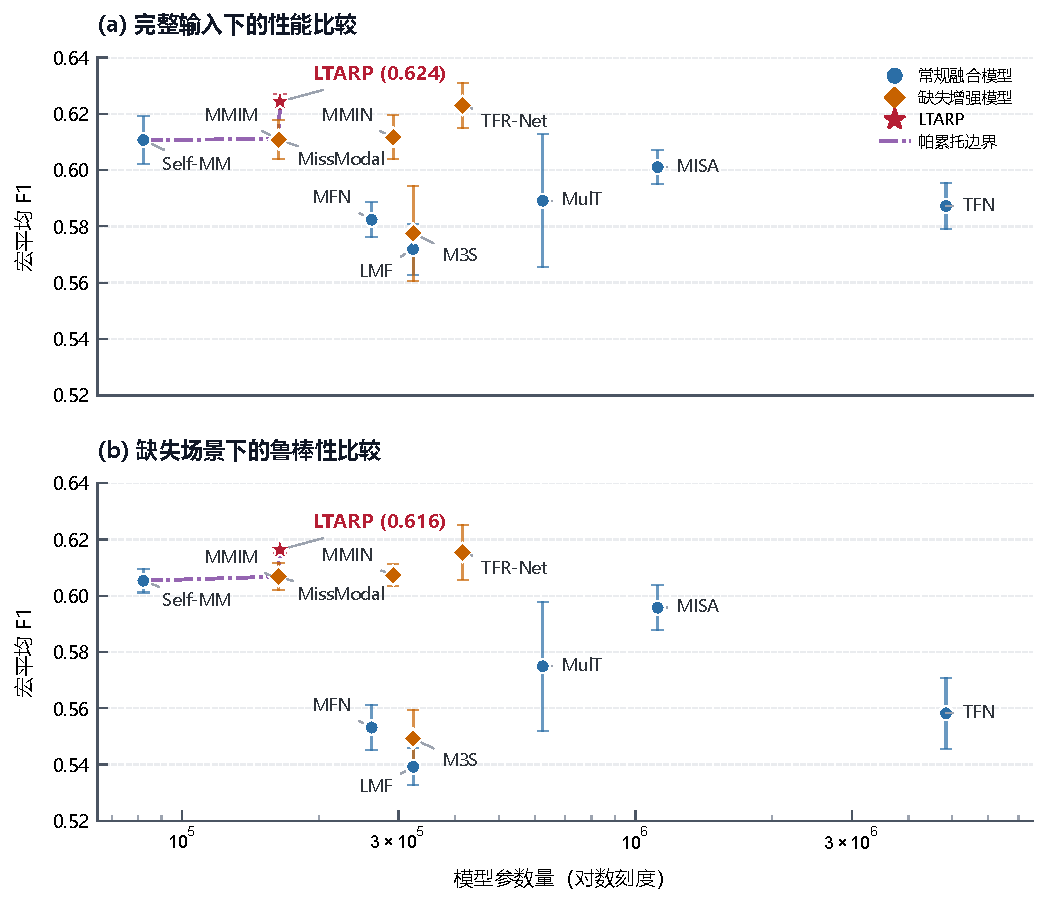
\includegraphics[width=.76\textwidth]{figures/q2/fig15_q2_parameter_macro_f1.pdf}
\caption{公开多模态模型的参数规模与宏平均 F1比较。（a）完整输入验证集；（b）54种连续缺失场景平均。横轴为总参数量（对数尺度），误差线为三随机种子的样本标准差。}
\label{fig:q2_params}\end{figure}
\FloatBarrier

\subsection{附件3预测}\label{subsec:q2_attachment3}
\subsubsection{文本特征重构与核验}
\QTwoParagraph 完成上述验证与模型选择后，将LTARP用于附件3的30条无标签样本。对齐版提供\texttt{text\_bert}词元输入，以及\texttt{audio}和\texttt{vision}数值特征。单样本的\texttt{text\_bert}形状为$3\times50$，三行依次为词元编号、有效位掩码和词元类型编号，并非模型所需的$50\times768$连续文本表示。因此，使用已验证的\texttt{bert-base-uncased}接口编码有效词元前缀，取最后隐层逐词元表示，再在填充后缀补零至$50\times768$；语音、视觉特征及有效位掩码保持原样。

\QTwoParagraph 已有接口检查使用附件4中20条同时包含\texttt{text\_bert}和预计算\texttt{text}的无标签样本，逐行比较全部604个有效槽位；604/604个重构行的最大余弦相似度位置均为同索引，特征最大绝对差为$3.0041\times10^{-5}$、RMSE为$8.3977\times10^{-7}$。输入同一固定参数模型后，分类logits最大绝对差为$2.44\times10^{-6}$，回归为$1.12\times10^{-6}$。该数值检查支持词元编码与既有文本特征接口的衔接，附件3随后沿此固定路径完成推理。

\subsubsection{预测结果汇总}
\QTwoParagraph 30条样本预测为消极、中性和积极的数量分别为7、11和12，对应23.33\%、36.67\%和40.00\%。连续情感强度均值为$+0.123114$、样本标准差为0.611792，范围为$[-1.642545,+1.539758]$；平均分类置信度为0.624599。类别与连续情感强度由两个输出头独立预测，推理阶段不使用回归值符号对分类结果进行二次修正。逐样本类别、连续情感强度和置信度见表~\ref{tab:q2_attachment3_all}，与独立CSV保存的同批结果对应。附件3不提供真实标签，因此本节仅报告预测结果，不计算Accuracy、Macro-F1、MAE等监督评价指标。

\Needspace{36\baselineskip}
\begingroup\zihao{-4}\setlength{\tabcolsep}{7pt}
\begin{longtable}{@{}llrr@{}}
\caption{附件3全部30条无标签样本的最终预测}\label{tab:q2_attachment3_all}\\
\toprule
样本ID & 预测类别 & 连续情感强度 & 分类置信度\\
\midrule\endfirsthead
\multicolumn{4}{@{}l}{续表~\thetable}\\
\toprule
样本ID & 预测类别 & 连续情感强度 & 分类置信度\\
\midrule\endhead
\midrule\multicolumn{4}{r@{}}{续下页}\\\endfoot
\bottomrule\endlastfoot
\texttt{\detokenize{附件3_01}} & 消极 & -0.405876 & 0.7460\\
\texttt{\detokenize{附件3_02}} & 中性 & -0.144469 & 0.6501\\
\texttt{\detokenize{附件3_03}} & 中性 & -0.128127 & 0.6101\\
\texttt{\detokenize{附件3_04}} & 积极 & +0.514640 & 0.6097\\
\texttt{\detokenize{附件3_05}} & 消极 & -1.642545 & 0.9405\\
\texttt{\detokenize{附件3_06}} & 积极 & +0.765383 & 0.7435\\
\texttt{\detokenize{附件3_07}} & 中性 & +0.249776 & 0.4401\\
\texttt{\detokenize{附件3_08}} & 消极 & -0.337494 & 0.5324\\
\texttt{\detokenize{附件3_09}} & 积极 & +1.076601 & 0.8747\\
\texttt{\detokenize{附件3_10}} & 中性 & -0.178815 & 0.7725\\
\texttt{\detokenize{附件3_11}} & 中性 & +0.010376 & 0.5348\\
\texttt{\detokenize{附件3_12}} & 积极 & +0.922382 & 0.6466\\
\texttt{\detokenize{附件3_13}} & 积极 & +0.237651 & 0.4991\\
\texttt{\detokenize{附件3_14}} & 消极 & -0.550781 & 0.7443\\
\texttt{\detokenize{附件3_15}} & 积极 & +0.684222 & 0.7227\\
\texttt{\detokenize{附件3_16}} & 积极 & +1.539758 & 0.9228\\
\texttt{\detokenize{附件3_17}} & 消极 & -0.589950 & 0.4977\\
\texttt{\detokenize{附件3_18}} & 积极 & +0.246677 & 0.4397\\
\texttt{\detokenize{附件3_19}} & 消极 & -0.320886 & 0.4778\\
\texttt{\detokenize{附件3_20}} & 中性 & -0.246796 & 0.6422\\
\texttt{\detokenize{附件3_21}} & 积极 & +0.667961 & 0.7211\\
\texttt{\detokenize{附件3_22}} & 中性 & +0.186271 & 0.4059\\
\texttt{\detokenize{附件3_23}} & 中性 & +0.138655 & 0.6286\\
\texttt{\detokenize{附件3_24}} & 消极 & -0.458430 & 0.5284\\
\texttt{\detokenize{附件3_25}} & 中性 & +0.048311 & 0.5231\\
\texttt{\detokenize{附件3_26}} & 积极 & +0.574989 & 0.7292\\
\texttt{\detokenize{附件3_27}} & 积极 & +0.567220 & 0.6708\\
\texttt{\detokenize{附件3_28}} & 积极 & +0.397136 & 0.4846\\
\texttt{\detokenize{附件3_29}} & 中性 & +0.071600 & 0.4322\\
\texttt{\detokenize{附件3_30}} & 中性 & -0.202034 & 0.5667\\
\end{longtable}
\endgroup
\FloatBarrier

\subsection{本问小结}\label{subsec:q2_summary}
\QTwoParagraph 本问以附件2已对齐的三模态特征为起点，建立MMP双任务基线，并通过LTARP内容加权残差分支补充时间位置的信息差异。在共用融合与输出路径的基础上，第二阶段仅新增883个参数，形成完整输入和连续缺失输入下可直接评价的预测模型。

\QTwoParagraph 围绕54种连续缺失场景的比较表明，文本局部缺失的影响最明显，分类与回归对位置的响应有所不同。LTARP在宏平均 F1、MAE和Pearson上总体优于MMP，但提升幅度较小，不同随机初始化下仍存在一定波动。与公开方法的统一适配比较进一步体现了其性能与参数规模的折中。在此基础上，本问完成附件3全部30条无标签样本的预测，并为问题三的解释分析固定预测模型。

\FloatBarrier
\addtocontents{toc}{\protect\newpage}
\section{问题三：多模态情感预测的可解释分析与证据定位}\label{sec:q3}

\subsection{问题分析与总体方案}\label{subsec:q3_overview}
\QThreeParagraph 问题二已经完成三模态情感类别与连续强度预测。针对问题三，本问不再调整预测模型，而是固定问题二得到的模型参数，进一步分析不同模态和局部输入对当前预测结果的作用。解释对象是同一条样本在不同输入条件下的输出变化。

\QThreeParagraph 由于最终预测由文本、语音和视觉共同产生，仅有类别和连续强度还无法区分各模态的具体作用。本问需要回答：三种模态分别贡献多少，两种模态共同输入时是否产生额外作用，以及影响当前预测的信息位于哪些特征位置。因此，分析依次从模态贡献转向模态交互，再定位局部特征区间。

\QThreeParagraph 整体求解路线见图~\ref{fig:fig14_q3_heaf_framework}。输入为$50\times768$的文本特征、$50\times74$的语音特征和$50\times35$的视觉特征，先枚举8种模态组合计算Shapley贡献，再利用相同组合输出分析模态交互；随后对分类主导模态进行连续窗口遮挡，定位影响当前类别的特征区间。所选区间进一步通过随机等长窗口对照和删除实验检验，并结合跨种子比较观察结果稳定性，最后沿来源记录回查原文片段或未对齐特征行。预测与解释始终使用问题二的双任务模型，分类和回归分别采用各自的解释目标，使两种输出的作用方向都有明确含义。

\newpage % 保留原稿方法流程图前的分页
\begin{figure}[H]
  \centering
  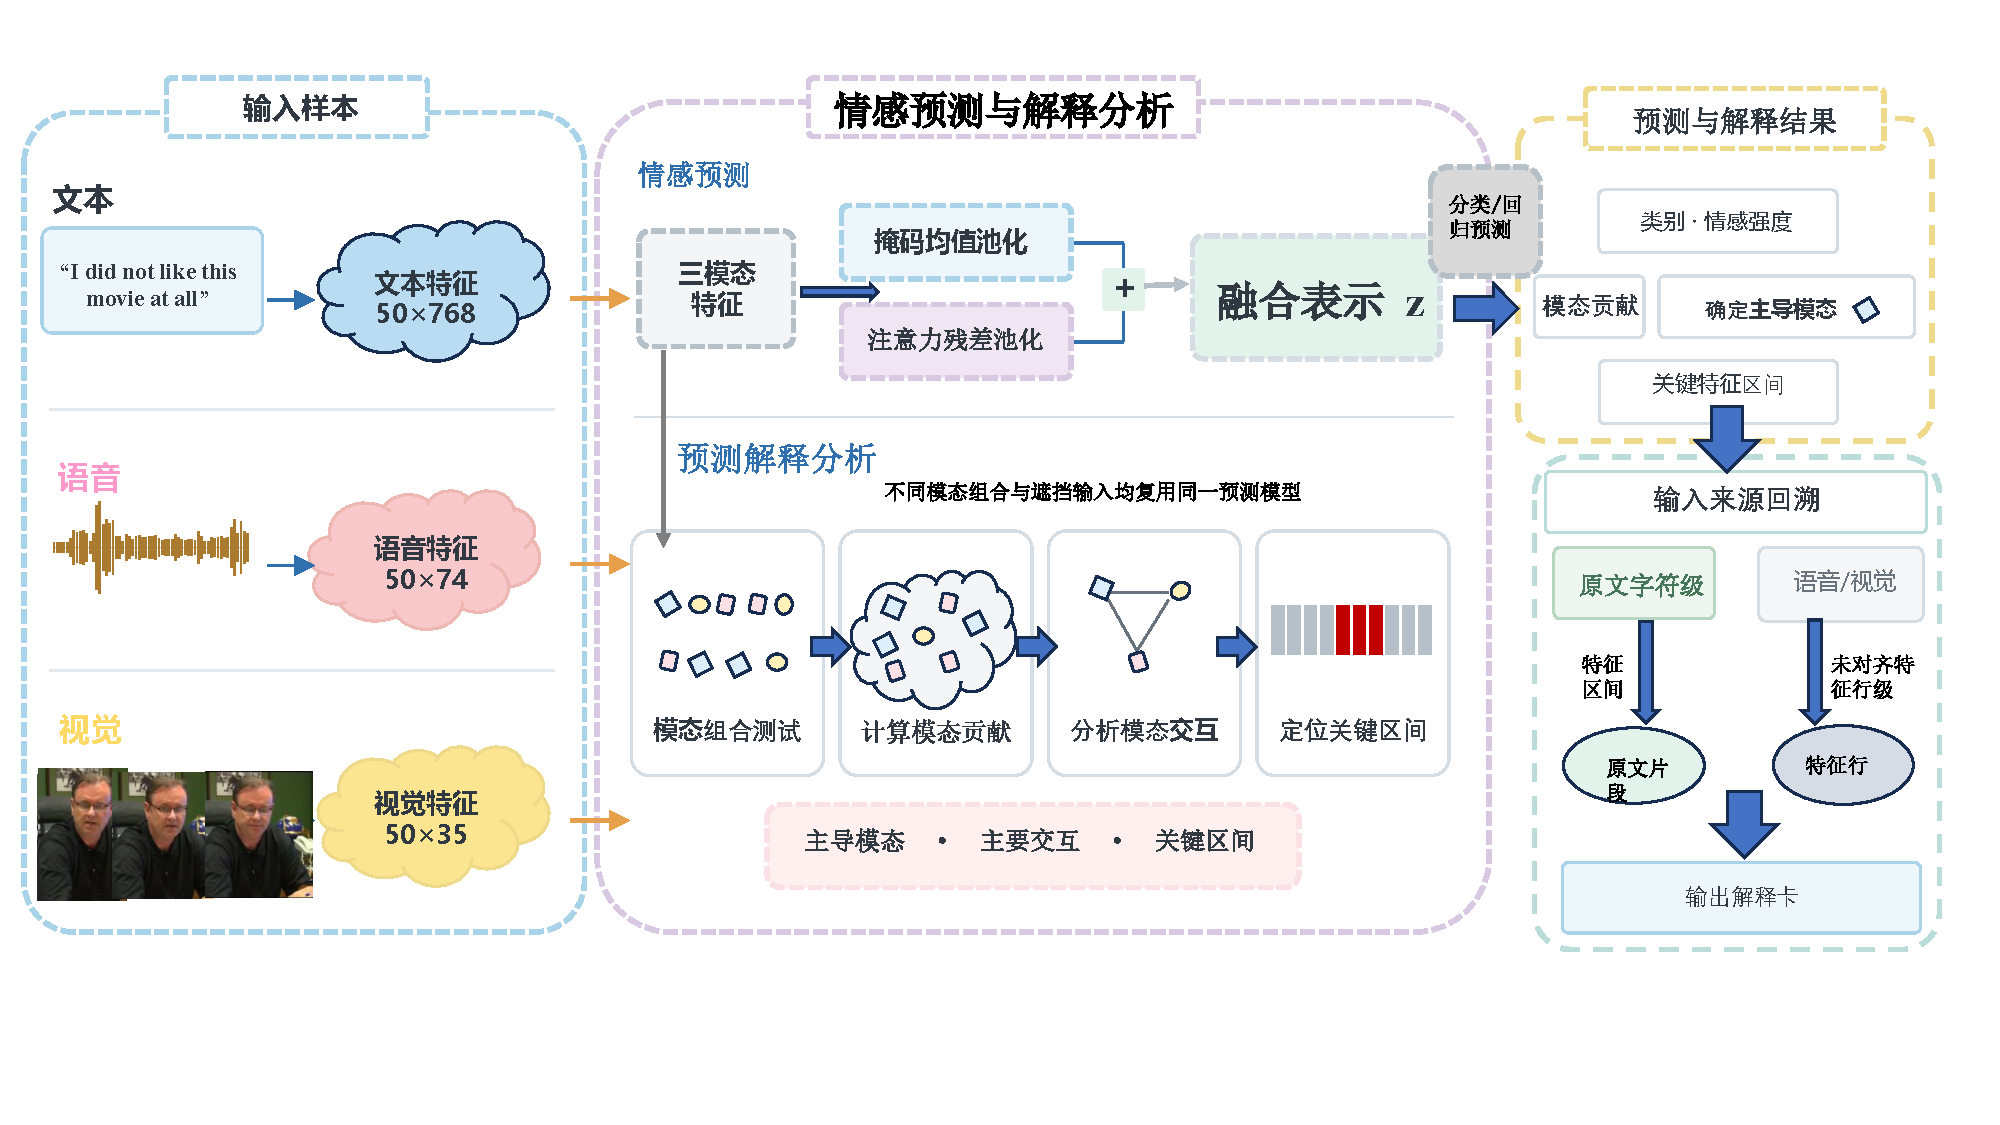
\includegraphics[width=1.0\textwidth]{figures/q3/fig14_q3_heaf_framework.pdf}
  \caption{固定预测模型的解释分析流程。输入为文本、语音和视觉特征，输出为预测类别、连续强度、模态贡献与关键特征区间。}
  \label{fig:fig14_q3_heaf_framework}
\end{figure}

\subsection{模态贡献分析}\label{subsec:q3_shapley}
\subsubsection{精确Shapley贡献}
\QThreeParagraph 只比较完整输入与去掉某一模态后的输出，得到的是该模态在另外两种模态都存在时的作用。一个模态的边际变化还可能取决于其他输入是否参与：单独有效的信息在联合输入中可能被替代，也可能在另一模态提供的条件下发挥更大作用。因此，需要把不同组合中的变化一起考虑。

Shapley贡献将一个模态加入不同组合时的边际变化加权平均。令$\mathcal M=\{T,A,V\}$分别表示文本、语音和视觉，$S\subseteq\mathcal M$为保留的模态集合，$v(S)$为相应组合的解释目标。三种模态只有$2^3=8$种组合，即空组合、三个单模态组合、三个双模态组合及完整组合，可以直接完整枚举，无需Monte Carlo采样近似。对模态$m$，其贡献为
\begin{equation}
\phi_m
=\sum_{S\subseteq\mathcal M\setminus\{m\}}
\frac{|S|!\,(2-|S|)!}{3!}
\bigl[v(S\cup\{m\})-v(S)\bigr].
\label{eq:q3_shapley}
\end{equation}
\QThreeParagraph 式中权重对应模态在不同加入顺序下遇到集合$S$的比例。三模态情况下，加入空组合或另外两模态均在场时的权重各为$1/3$，加入单模态组合时各为$1/6$。每个模态按相同规则计算，使单独作用与联合输入下的增量都参与贡献分配。

\QThreeParagraph 计算时，未保留模态只在有效位置清零，填充位置与原生零记录保持原样。空组合对应全部有效模态清零后的模型输出，作为本问的共同基准。精确计算满足$\sum_m\phi_m=v(\mathcal M)-v(\varnothing)$，用于检查贡献分配是否完整；该关系针对模型输出差，空组合的预测值本身由固定模型决定。

\subsubsection{解释目标与主导模态}
\QThreeParagraph 确定模态贡献的计算方式后，还需要为各模态组合规定一致的比较目标。由于分类与回归的输出形式不同，本文分别定义两类解释目标。分类解释固定完整输入预测的类别$c^\star$，所有模态组合均衡量对这一类别的支持程度。若只记录遮挡后类别是否翻转，许多尚未越过分类边界的变化会被忽略；采用分类对数优势（log-odds），则能保留当前类别相对于其他类别的连续变化。记$z_k(S)$为组合$S$下类别$k$的logit，回归直接使用连续强度预测$\widehat y^{\mathrm r}(S)$，两种目标定义为
\begin{equation}
v_{\mathrm c}(S)
=z_{c^\star}(S)-\log\!\sum_{k\ne c^\star}\exp z_k(S),
\qquad
v_{\mathrm r}(S)=\widehat y^{\mathrm r}(S).
\label{eq:q3_value}
\end{equation}
\QThreeParagraph 其中，分类目标等于$\log[p_{c^\star}(S)/(1-p_{c^\star}(S))]$。即使某个组合使模型改判其他类别，$c^\star$也保持不变，前后差值仍指向同一个解释对象。回归目标保留模型输出的原始尺度，因此分类和回归分别计算贡献并确定主导模态。

\QThreeParagraph 分类正贡献表示该模态支持当前类别，负贡献表示其反向作用；回归正、负贡献分别对应连续强度向正、负方向的变化。贡献的绝对值表示变化幅度，符号保留方向。例如，某模态可以增强中性判断，同时使连续强度降低，两个结果分别依据各自目标解读。

\QThreeParagraph 分类主导模态优先取最大正Shapley贡献；若三种贡献均非正，则取绝对贡献最大者，并标明其非支持性质。回归主导模态取绝对贡献最大者。两类选择遇到并列时，均按文本、语音、视觉的固定顺序处理。后续连续窗口遮挡以分类主导模态为分析对象，回归输出用于观察同一区间对强度的影响。

\QThreeParagraph 主导模态确定局部分析对象，三路贡献仍共同保留。非主导模态可能提供较小的同向支持，也可能产生较大的反向作用；只报告最大值会掩盖这种差异。逐样本表因此列出完整的三模态贡献，便于结合大小和方向阅读当前预测。

\subsection{模态交互分析}\label{subsec:q3_interaction}
Shapley贡献将完整输入相对空输入的预测变化分配给各模态，其中已经包含联合输入的影响。模态交互另行回答：两种模态共同输入后，相对于各自作用的简单相加，多出了什么变化。贡献较大的模态与其他模态仍可能呈现正或负交互，二者描述的方面不同。

\QThreeParagraph 本文考察文本--语音、文本--视觉和语音--视觉三对关系。对模态$i,j$及剩余模态$k$，分别计算第三模态缺席和在场时的二阶差，再取平均：
\begin{equation}
\begin{aligned}
I_{ij}=\tfrac12\{&
v(\{i,j\})-v(\{i\})-v(\{j\})+v(\varnothing)\\
&+v(\mathcal M)-v(\{i,k\})-v(\{j,k\})+v(\{k\})\}.
\end{aligned}
\label{eq:q3_interaction}
\end{equation}
\QThreeParagraph 正交互表示联合输入产生的输出变化高于相应加性基准，负交互表示低于这一基准。符号针对式~\eqref{eq:q3_value}的解释目标，具体原因需结合样本输入判断；分类和回归分别计算。

\QThreeParagraph 附件2验证集728条样本的交互统计见表~\ref{tab:q3_interaction}。平均交互概括作用的平均大小，主要符号比例为该方向在样本中出现的频率。文本--视觉在两个目标下平均为正，其中分类均值为$+0.0781$；语音--视觉的平均方向则由分类负向转为回归正向。可见，共同输入对类别支持与连续强度的影响并不完全一致。

\begin{table}[H]
\centering\zihao{-4}
\caption{附件2验证集分类与回归解释目标的二阶模态交互（$n=728$）}
\label{tab:q3_interaction}
\begin{tabular}{@{}llrrl@{}}
\toprule
解释目标 & 模态对 & 平均交互 & 主要符号比例 & 主要符号\\
\midrule
\multirow{3}{*}{分类} & 文本--语音 & $-0.0706$ & $69.4\%$ & 负\\
 & 文本--视觉 & $+0.0781$ & $60.3\%$ & 正\\
 & 语音--视觉 & $-0.0372$ & $64.4\%$ & 负\\
\addlinespace
\multirow{3}{*}{回归} & 文本--语音 & $-0.1592$ & $85.7\%$ & 负\\
 & 文本--视觉 & $+0.0503$ & $65.4\%$ & 正\\
 & 语音--视觉 & $+0.0592$ & $84.1\%$ & 正\\
\bottomrule
\end{tabular}
\end{table}

\QThreeParagraph 总体方向也不能代替单样本结果。文本--视觉的分类交互有60.3\%为正，仍有相当一部分样本呈现其他方向。群体统计用于概括这批输入的共同特点，逐条解释则保留样本自身的交互量，与其模态贡献和局部位置一起阅读。

\subsection{连续窗口遮挡与关键区间定位}\label{subsec:q3_temporal}
\QThreeParagraph 模态贡献比较整路输入的作用，尚未指出重要信息位于序列何处。本文在分类主导模态内部遮挡连续特征区间，保持其他模态及窗口外输入不变，通过输出变化定位局部影响。连续窗口覆盖相邻特征，可以观察一段输入共同被去除后的响应，避免把片段作用仅归于单个槽位。

\QThreeParagraph 对样本$i$，有效长度为$L_i$，窗口宽度为$w_i=\max(1,\operatorname{round}(0.30L_i))$，滑动步长为1。窗口只在有效序列内生成，依次覆盖从起点到末端的所有可用连续区间。有效掩码保持不变，清零操作表示去除当前窗口的观测内容；原生零记录沿用输入原值，填充位置不进入候选窗口。记$g(\mathbf x)$为固定类别的分类对数优势，窗口$W$的遮挡效应为
\begin{equation}
D_i(W)=g(\mathbf x_i)-g\!\left(\mathbf x_i^{\setminus W}\right),
\label{eq:q3_occlusion}
\end{equation}
\QThreeParagraph 其中$\mathbf x_i^{\setminus W}$仅将分类主导模态在窗口内的有效特征清零。$D_i(W)>0$表示删除后当前类别支持下降，窗口原本支持该预测；$D_i(W)<0$表示删除后支持上升，窗口原本对当前类别起反向作用。

\QThreeParagraph 若存在正效应窗口，选择$D_i(W)$最大的窗口；若所有窗口均无正效应，则选择绝对效应最大的窗口并标注方向。平局时取最早位置。结果使用从零开始的对齐索引$[a,b)$表示，包含$a$至$b-1$位置。对每个有效槽位，将覆盖该位置的窗口效应最大值记为局部曲线；这条曲线描述连续遮挡下的响应，窗口之间可以重叠。

\QThreeParagraph 窗口比例通过附件2验证集的设计子集确定。既有实验比较$\{0.10,0.20,0.30\}$，按所选窗口相对随机等长窗口的平均分类对数优势下降差选择比例；三者依次为0.268837、0.366684和0.440487，因此选定0.30。随后固定该比例，在独立验证子集报告结果，并用于附件4。该选择依据对应局部分类影响，实际区间宽度仍随每条样本的有效长度变化。

\QThreeParagraph 区间索引首先定位的是模型接收的特征，具体输入来源在第~\ref{subsec:q3_grounding}节回溯。对同一所选窗口，回归同时记录完整输出减遮挡输出的有符号变化及其绝对值，分别描述强度移动方向和幅度。

\QThreeParagraph 三模态Shapley只需8种组合，三对交互复用这些输出。连续窗口的候选数为$L_i-w_i+1$，随有效长度线性增加。在最长50位的序列上，单样本的贡献计算与局部定位均可直接遍历；模型参数、有效掩码、解释目标及窗口规则固定后，同一输入的结果可按上述步骤复算。

\subsection{关键区间的干预验证与稳定性分析}\label{subsec:q3_faithfulness}
\QThreeParagraph 前述模态贡献和连续窗口遮挡给出了对当前预测起主要作用的模态及关键特征区间，但这些位置是否对应更明显的模型响应，还需要通过独立验证子集上的干预对照进行检验。

\subsubsection{实验设计}
\QThreeParagraph 为此，本文固定问题二的seed 42模型。其在附件2验证集上的基础性能见表~\ref{tab:q3_predictor}，其中中性类别F1和召回率低于另两类，是主要分类误差来源之一。基础性能提供预测质量背景，下述实验评价所选位置与该模型输出之间的对应关系。

\begin{table}[H]
\centering\zihao{-4}
\setlength{\tabcolsep}{6pt}
\caption{Q3固定预测模型在附件2验证集上的基础性能（seed 42，$n=728$）}
\label{tab:q3_predictor}
\begin{tabular}{@{}cccc@{}}
\toprule
Accuracy & Macro-F1 & MAE & Pearson\\
\midrule
0.648352 & 0.623435 & 0.608260 & 0.646170\\
\midrule
消极F1 & 中性F1 & 积极F1 & 中性召回率\\
\midrule
0.689655 & 0.467836 & 0.712813 & 0.434783\\
\bottomrule
\end{tabular}
\end{table}

\QThreeParagraph 附件2验证集共728条片段，按video ID分为设计子集和独立验证子集。前者含332条片段、113个视频，后者含396条片段、126个视频，两组video ID无重叠。同一视频的片段可能共享说话人和场景，按视频分组可以避免这些共同条件跨越两组。设计子集用于确定窗口比例，独立验证子集用于报告最终干预结果；这里的独立性针对窗口比例选择与解释验证。

\QThreeParagraph 对每条独立验证样本，从同一主导模态的有效序列中随机抽取32次等长窗口，以其平均效应作为对照。等长条件控制被遮挡位置的数量，使比较集中于位置差异。另按局部曲线从高到低删除10\%、20\%、30\%、40\%的有效位置，与删除同样数量的随机位置比较，观察累计影响。随机种子为20260924，95\%区间采用按视频分组的1000次自助采样，以保留同视频片段的组内关联。

\subsubsection{核心干预结果}
\QThreeParagraph 表~\ref{tab:q3_faithfulness}中，三个分类指标方向一致：所选窗口删除后引起的输出变化大于随机等长窗口。分类对数优势平均下降差为0.400735，95\%区间为$[0.3635,0.4372]$；置信度和当前类别logit也呈同向差异。这说明固定模型对所选位置更敏感。由于所选窗口本身依据遮挡效应确定，该比较主要用于观察这些位置对固定模型输出的敏感程度。上述干预结果描述输入变化与固定模型输出之间的关系，不用于推断现实情感形成的因果机制。

\begin{table}[H]
\centering\zihao{-4}
\setlength{\tabcolsep}{4pt}
\caption{附件2独立验证子集的解释干预一致性结果（396条片段；按视频分组的95\%自助采样区间）}
\label{tab:q3_faithfulness}
\begin{tabular}{@{}lcccc@{}}
\toprule
输出量 & 所选窗口 & 随机等长窗口 & 平均差 & 95\%区间\\
\midrule
分类对数优势下降 & 0.482771 & 0.082036 & 0.400735 & $[0.3635,0.4372]$\\
分类置信度下降 & 0.093286 & 0.015567 & 0.077718 & $[0.0712,0.0843]$\\
分类logit下降 & 0.292982 & 0.053294 & 0.239688 & $[0.2195,0.2603]$\\
回归有符号变化 & 0.002082 & 0.020177 & $-0.018095$ & $[-0.0526,0.0141]$\\
回归绝对变化 & 0.202760 & 0.099215 & 0.103545 & $[0.0883,0.1203]$\\
\bottomrule
\end{tabular}
\end{table}

\QThreeParagraph 回归结果需要区分方向与幅度。有符号变化差为$-0.018095$，区间跨零，表明删除后连续强度没有统一的移动方向；不同样本的正、负变化可能在平均时抵消。绝对变化差为$+0.103545$，说明同一所选区间仍引起更大的强度数值变化。局部窗口依据分类目标选出，回归结果描述该窗口对另一输出的响应。

\QThreeParagraph 删除曲线进一步显示影响随去除范围的变化。删除比例由10\%增至40\%时，高影响位置与随机位置的平均分类对数优势下降差依次为0.108296、0.237758、0.418076和0.465465（图~\ref{fig:fig15_q3_faithfulness_validation}）。差异在四个比例下均为正并逐渐扩大，说明高影响位置的累计删除持续改变当前类别支持。曲线按局部效应排序后删除多个位置，与表中的单个连续窗口对照采用不同的删除集合。

\begin{figure}[H]
  \centering
  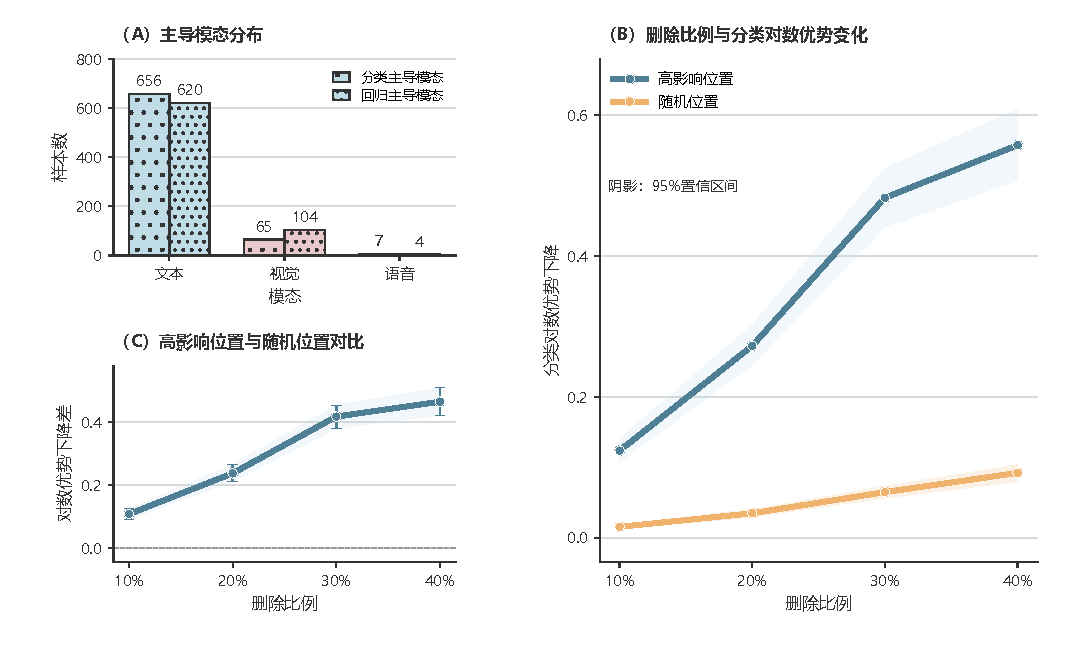
\includegraphics[width=1.0\textwidth]{figures/q3/fig15_q3_faithfulness_validation.pdf}
  \caption{主导模态与删除干预结果。（A）728条验证样本的分类、回归主导模态计数；（B）396条独立验证样本的删除比例曲线；（C）高影响位置与随机位置的配对下降差。阴影为按视频分组的95\%自助采样区间。}
  \label{fig:fig15_q3_faithfulness_validation}
\end{figure}

\subsubsection{跨种子稳定性}
\QThreeParagraph 使用既有seed 43、44模型与seed 42比较，保持独立验证样本和窗口比例相同。表~\ref{tab:q3_seed_stability}同时报告主导模态一致率、Shapley贡献的Spearman秩相关系数及关键区间交并比（IoU）。秩相关先在每条样本的三个贡献值之间计算，再对样本取均值；分类相关仅比较两个模型预测类别相同的样本，使贡献排序对应同一类别。

\begin{table}[H]
\centering\zihao{-4}
\setlength{\tabcolsep}{4pt}
\caption{附件2独立验证子集的跨种子解释稳定性（seed 42分别与43、44比较；$n=396$）}
\label{tab:q3_seed_stability}
\begin{tabular}{@{}llccc@{}}
\toprule
解释目标 & 种子对 & 主导模态一致率 & Shapley秩相关 & 关键区间IoU\\
\midrule
\multirow{2}{*}{分类} & 42/43 & 0.869 & 0.818 & 0.579\\
 & 42/44 & 0.831 & 0.783 & 0.527\\
\multirow{2}{*}{回归} & 42/43 & 0.778 & 0.745 & ---\\
 & 42/44 & 0.783 & 0.760 & ---\\
\bottomrule
\end{tabular}
\par\vspace{2pt}{\zihao{-4} 秩相关为逐样本三模态Shapley贡献的Spearman系数均值。分类仅统计两种子预测类别一致的样本；IoU为主导模态相同时的区间交并比，模态不同时记为0；回归未单独定义关键区间。}
\end{table}

\QThreeParagraph 分类主导模态一致率为0.869和0.831，区间IoU为0.579和0.527；回归主导模态一致率为0.778和0.783。模态选择相对稳定，具体窗口边界更敏感。主导模态只在三路输入之间比较，窗口却要从多个重叠候选中选出最大效应位置；若相邻窗口作用接近，初始化导致的小幅输出变化就可能改变边界。局部区间因此宜结合模态贡献和连续曲线阅读。

\subsection{关键位置的输入来源回溯}\label{subsec:q3_grounding}
\QThreeParagraph 连续窗口遮挡给出对齐特征中的索引，来源回溯将这些位置连接到可阅读的文本或已有特征记录。附件4的对应关系来自其自身的词元输入、原文和未对齐特征，按三种模态现有记录能够确认的精度分别报告。

\QThreeParagraph 文本采用“对齐特征槽位$\rightarrow$BERT词元$\rightarrow$原文字符区间”的映射。利用固定BERT编码路径重构文本特征后，对20条样本的604个有效槽位进行逐行比较，全部行的最大余弦相似度匹配位置均为同索引。平均同索引余弦为0.999999994，最大绝对差为$3.0041\times10^{-5}$，均方根误差为$8.3977\times10^{-7}$。这些数值支持对齐文本行与词元位置的对应关系。

\QThreeParagraph 词元到原文的字符跨度由分词器提供，因而可将所选窗口内的实际词元回到原文字符区间。特殊词元本身不产生原文片段，窗口内的文本以真实字符跨度读取。这一处理使结果既保留模型中的槽位索引，也给出可直接阅读的文字；两种坐标描述的是同一输入在不同表示中的位置。

\QThreeParagraph 语音和视觉通过逐行特征匹配回到未对齐数组。附件4的564/564个非零语音对齐行、534/534个非零视觉对齐行，都能在对应样本的未对齐特征中找到唯一且逐元素相等的行。这种对应依赖实际特征值，不要求把50个槽位均分到视频时长；原生零行则保留原记录，不赋予未经确认的来源索引。

\QThreeParagraph 据此，文本位置报告为“原文字符级”，语音和视觉位置报告为“未对齐特征行级”。现有音视频来源记录还缺少从未对齐行到音频秒数或视频帧时间的可靠映射，位置精度止于特征行。典型案例图保留的视频画面用于显示上下文，其选取独立于关键特征区间。

\subsection{附件4预测与解释结果}\label{subsec:q3_attachment4}
\QThreeParagraph 完成解释方法及独立验证后，本文将固定的预测与解释流程应用于附件4的20条无标签样本，其中预测为消极、中性和积极的数量分别为7、5和8，分布见表~\ref{tab:q3_attachment4}。全部类别、连续强度和分类置信度列于表~\ref{tab:q3_attachment4_all}；分类Shapley贡献与关键特征区间列于表~\ref{tab:q3_attachment4_explanations}。附件4没有真实标签，因此本节报告预测及解释结果，不计算Accuracy、F1、MAE或Pearson等监督评价指标。

\QThreeParagraph 分类主导模态为文本、视觉、语音的样本数分别为19、1、0，回归分别为18、2、0。分类主导模态与回归主导模态在17条样本上一致，占85\%，其余3条样本的两类主导模态不同。表中$\phi_T,\phi_A,\phi_V$均对应分类对数优势，保留符号以显示同向支持和反向作用。

\begin{table}[H]
\centering\zihao{-4}
\caption{附件4的无标签预测及解释摘要（共20条样本）}
\label{tab:q3_attachment4}
\begin{tabular}{@{}llrr@{}}
\toprule
统计项 & 类别或来源 & 数量 & 比例\\
\midrule
\multirow{3}{*}{预测情感类别} & 消极 & 7 & 35\%\\
 & 中性 & 5 & 25\%\\
 & 积极 & 8 & 40\%\\
\addlinespace
\multirow{3}{*}{分类主导模态} & 文本 & 19 & 95\%\\
 & 语音 & 0 & 0\%\\
 & 视觉 & 1 & 5\%\\
\addlinespace
\multirow{3}{*}{回归主导模态} & 文本 & 18 & 90\%\\
 & 语音 & 0 & 0\%\\
 & 视觉 & 2 & 10\%\\
\addlinespace
\multirow{2}{*}{分类关键位置来源} & 原文字符级 & 19 & 95\%\\
 & 未对齐特征行级 & 1 & 5\%\\
\bottomrule
\end{tabular}
\end{table}

\begin{table}[H]
\centering\zihao{-4}\setlength{\tabcolsep}{7pt}
\caption{附件4全部20条无标签样本的预测结果}
\label{tab:q3_attachment4_all}
\begin{tabular}{@{}llrr@{}}
\toprule
样本ID & 预测类别 & 情感强度 & 分类置信度\\
\midrule
\texttt{\detokenize{01}} & 中性 & +0.177915 & 0.5359\\
\texttt{\detokenize{02}} & 消极 & -0.027301 & 0.3898\\
\texttt{\detokenize{03}} & 中性 & -0.064430 & 0.5441\\
\texttt{\detokenize{04}} & 消极 & -0.398096 & 0.6741\\
\texttt{\detokenize{05}} & 积极 & +0.886586 & 0.7131\\
\texttt{\detokenize{06}} & 积极 & +0.759221 & 0.7287\\
\texttt{\detokenize{07}} & 积极 & +0.799232 & 0.7699\\
\texttt{\detokenize{08}} & 积极 & +0.678992 & 0.7512\\
\texttt{\detokenize{09}} & 消极 & -1.987819 & 0.9671\\
\texttt{\detokenize{10}} & 消极 & -1.556107 & 0.9453\\
\texttt{\detokenize{11}} & 消极 & -0.965641 & 0.8577\\
\texttt{\detokenize{12}} & 消极 & -0.981858 & 0.8488\\
\texttt{\detokenize{13}} & 中性 & +0.173788 & 0.5675\\
\texttt{\detokenize{14}} & 中性 & +0.154869 & 0.5568\\
\texttt{\detokenize{15}} & 积极 & +1.267568 & 0.8941\\
\texttt{\detokenize{16}} & 消极 & -2.030377 & 0.9670\\
\texttt{\detokenize{17}} & 积极 & +1.656759 & 0.9493\\
\texttt{\detokenize{18}} & 中性 & -0.158624 & 0.5781\\
\texttt{\detokenize{19}} & 积极 & +0.276115 & 0.3840\\
\texttt{\detokenize{20}} & 积极 & +0.875848 & 0.8013\\
\bottomrule
\end{tabular}
\end{table}


\begin{table}[H]
\centering\zihao{-4}\setlength{\tabcolsep}{3.5pt}
\caption{附件4全部20条样本的分类贡献与输入来源；区间为从零开始的对齐特征槽位$[a,b)$}
\label{tab:q3_attachment4_explanations}
\begin{tabular}{@{}lrrrlcl@{}}
\toprule
ID & $\phi_T$ & $\phi_A$ & $\phi_V$ & 主导模态 & 关键区间 & 输入来源\\
\midrule
\texttt{\detokenize{01}} & +0.4448 & +0.0283 & +0.0097 & 文本 & $[17,24)$ & 原文字符级\\
\texttt{\detokenize{02}} & -0.1971 & +0.2277 & +0.8294 & 视觉 & $[1,7)$ & 未对齐特征行级\\
\texttt{\detokenize{03}} & +0.6919 & -0.1267 & -0.0492 & 文本 & $[0,10)$ & 原文字符级\\
\texttt{\detokenize{04}} & +1.9249 & +0.1198 & -0.0096 & 文本 & $[20,28)$ & 原文字符级\\
\texttt{\detokenize{05}} & +1.1092 & -0.3336 & +0.6619 & 文本 & $[0,5)$ & 原文字符级\\
\texttt{\detokenize{06}} & +2.2790 & -0.2529 & -0.5109 & 文本 & $[14,25)$ & 原文字符级\\
\texttt{\detokenize{07}} & +1.6925 & -0.3365 & +0.3790 & 文本 & $[13,28)$ & 原文字符级\\
\texttt{\detokenize{08}} & +2.4908 & -0.2620 & -0.5967 & 文本 & $[8,12)$ & 原文字符级\\
\texttt{\detokenize{09}} & +4.0872 & +0.4352 & +0.1656 & 文本 & $[2,8)$ & 原文字符级\\
\texttt{\detokenize{10}} & +3.6626 & +0.4324 & +0.0621 & 文本 & $[21,31)$ & 原文字符级\\
\texttt{\detokenize{11}} & +2.0970 & +0.2465 & +0.7610 & 文本 & $[1,6)$ & 原文字符级\\
\texttt{\detokenize{12}} & +2.1874 & -0.0032 & +0.8495 & 文本 & $[31,44)$ & 原文字符级\\
\texttt{\detokenize{13}} & +0.5928 & +0.0180 & +0.0000 & 文本 & $[0,10)$ & 原文字符级\\
\texttt{\detokenize{14}} & +1.5361 & +0.0546 & -1.0233 & 文本 & $[1,12)$ & 原文字符级\\
\texttt{\detokenize{15}} & +2.9847 & -0.3149 & -0.0090 & 文本 & $[14,21)$ & 原文字符级\\
\texttt{\detokenize{16}} & +3.8314 & +0.4557 & +0.3986 & 文本 & $[8,12)$ & 原文字符级\\
\texttt{\detokenize{17}} & +3.4202 & -0.1421 & +0.1781 & 文本 & $[9,17)$ & 原文字符级\\
\texttt{\detokenize{18}} & +0.8431 & -0.0933 & -0.0955 & 文本 & $[6,21)$ & 原文字符级\\
\texttt{\detokenize{19}} & +0.6310 & -0.4071 & -0.1692 & 文本 & $[29,41)$ & 原文字符级\\
\texttt{\detokenize{20}} & +2.0873 & -0.2851 & +0.1195 & 文本 & $[0,14)$ & 原文字符级\\
\bottomrule
\end{tabular}
\end{table}


\Needspace{5\baselineskip}
\QThreeParagraph 同一类别内部的输出也有明显差异。样本02与样本09均被预测为消极，连续强度却分别为$-0.027301$和$-1.987819$，分类置信度分别为0.3898和0.9671。类别、强度和置信度描述不同方面，逐样本结果将它们分别保留，避免用一个类别标签替代连续输出。

\subsection{典型样本分析与本问小结}\label{subsec:q3_cases}
\QThreeParagraph 附件4多数样本由文本主导，但也存在视觉主导的个例。为比较不同模态主导时的贡献和来源回溯结果，图~\ref{fig:fig16_q3_case_explanations}选取文本主导的样本14和视觉主导的样本02进行分析。

\QThreeParagraph 样本14预测为中性，连续强度为$+0.154869$。三模态分类贡献为$\phi_T=+1.536072$、$\phi_A=+0.054570$、$\phi_V=-1.023311$，文本是主要正向输入，视觉对当前中性类别起反向作用，语音贡献较小。文本关键特征区间$[1,12)$对应原文字符$[0,38)$，片段为“He is the co-founder of Rossen and Vet”。所选文本区间可进一步回查到上述原文片段，从而明确模型中主要文本支持对应的具体内容。贡献的正向指对中性类别的支持，与积极情感标签含义不同。

\QThreeParagraph 样本02预测为消极，连续强度为$-0.027301$。其贡献为$\phi_T=-0.197115$、$\phi_A=+0.227718$、$\phi_V=+0.829375$，视觉支持最大，语音同向但较小，文本产生反向作用。视觉关键特征区间$[1,7)$包含对齐槽位1--6，可逐行对应到未对齐视觉特征行36--41。因此，视觉主导样本的关键位置可以进一步对应到已有的未对齐视觉特征记录。图中的场景画面提供观看上下文。

\begin{figure}[H]
  \centering
  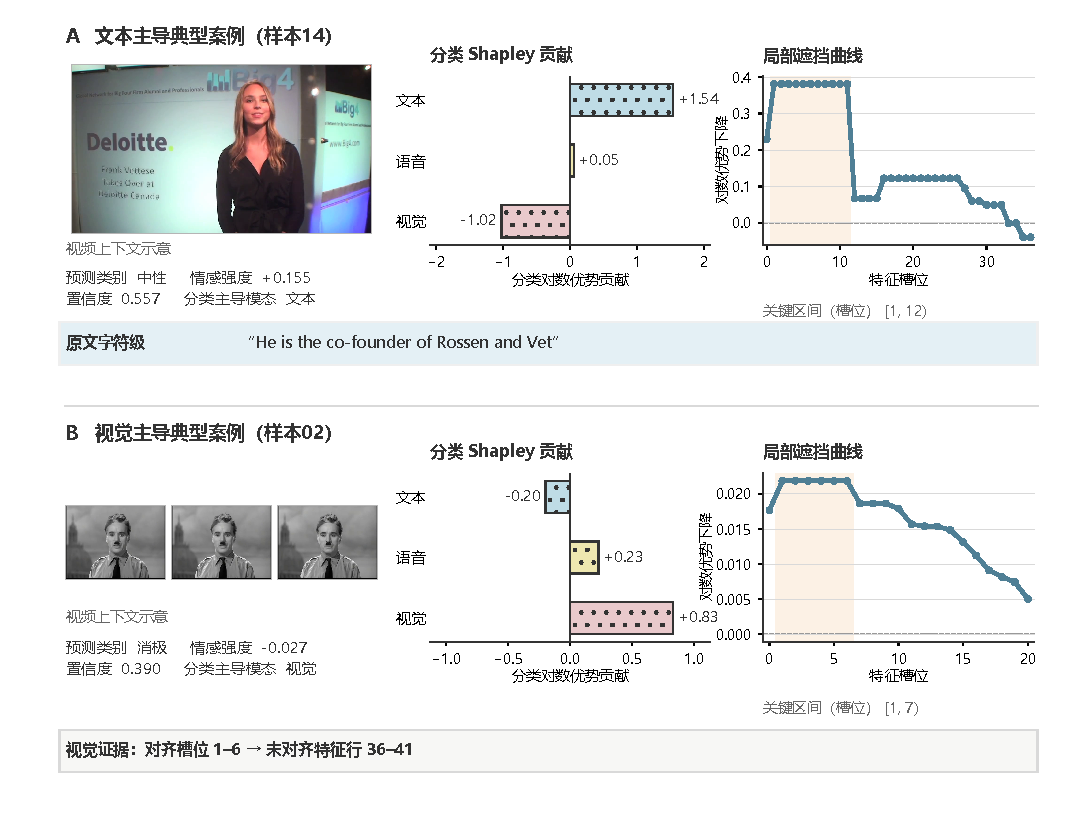
\includegraphics[width=1.0\textwidth]{figures/q3/fig16_q3_case_explanations.pdf}
  \caption{附件4的典型样本。（A）样本14的文本贡献、局部遮挡曲线与原文片段；（B）样本02的视觉贡献、局部遮挡曲线与未对齐特征行对应。浅色带标出所选特征区间，视频画面为上下文示意。}
  \label{fig:fig16_q3_case_explanations}
\end{figure}

\QThreeParagraph 两个案例的回溯终点不同：样本14可以直接读取原文字符，样本02当前可查到未对齐视觉特征行。同一遮挡方法给出特征区间，而能够进一步阅读或展示何种输入，取决于该模态保存的来源记录。

\QThreeParagraph 本问固定问题二的预测模型，以模态组合输出计算三模态贡献与两两交互，再用连续窗口遮挡定位局部影响。随机等长窗口、删除曲线和跨种子比较分别考察局部响应、累计影响及初始化变化，使解释结果可以结合模型的实际输出评估。

\QThreeParagraph 附件4的20条样本均得到类别、连续强度、模态贡献和关键区间，并按已有来源记录连接到原文或未对齐特征行。逐样本的同向与反向贡献、不同主导模态及不同位置，共同呈现固定模型使用三路输入的差异，也为检查具体预测提供了可复查的记录。

\FloatBarrier
\clearpage
\phantomsection\label{front:references}
\addcontentsline{toc}{section}{参考文献}
{\zihao{-4}
\begin{thebibliography}{99}

\bibitem{radford2023whisper}
Alec Radford, Jong~Wook Kim, Tao Xu, Greg Brockman, Christine McLeavey, and
  Ilya Sutskever.
\newblock Robust speech recognition via large-scale weak supervision.
\newblock In {\em Proceedings of the 40th International Conference on Machine
  Learning}, volume 202 of {\em Proceedings of Machine Learning Research},
  pages 28492--28518. PMLR, 2023.

\bibitem{liu2019roberta}
Yinhan Liu, Myle Ott, Naman Goyal, Jingfei Du, Mandar Joshi, Danqi Chen, Omer
  Levy, Mike Lewis, Luke Zettlemoyer, and Veselin Stoyanov.
\newblock {RoBERTa}: A robustly optimized {BERT} pretraining approach.
\newblock {\em arXiv preprint arXiv:1907.11692}, 2019.

\bibitem{chen2022wavlm}
Sanyuan Chen, Chengyi Wang, Zhengyang Chen, Yu~Wu, Shujie Liu, Zhuo Chen, Jinyu
  Li, Naoyuki Kanda, Takuya Yoshioka, Xiong Xiao, Jian Wu, Long Zhou, Shuo Ren,
  Yanmin Qian, Yao Qian, Jian Wu, Michael Zeng, Xiangzhan Yu, and Furu Wei.
\newblock {WavLM}: Large-scale self-supervised pre-training for full stack
  speech processing.
\newblock {\em IEEE Journal of Selected Topics in Signal Processing},
  16(6):1505--1518, 2022.

\bibitem{tschannen2025siglip2}
Michael Tschannen, Alexey Gritsenko, Xiao Wang, Muhammad~Ferjad Naeem, Nikhil
  Alabdulmohsin, Nikhil Parthasarathy, Talfan Evans, Lucas Beyer, Ye~Xia, Basil
  Mustafa, Olivier H{\'e}naff, Jeremiah Harmsen, Andreas Steiner, and Xiaohua
  Zhai.
\newblock {SigLIP 2}: Multilingual vision-language encoders with improved
  semantic understanding, localization, and dense features.
\newblock {\em arXiv preprint arXiv:2502.14786}, 2025.

\bibitem{simeoni2025dinov3}
Oriane Sim{\'e}oni, Huy~V. Vo, Maximilian Seitzer, Federico Baldassarre, Maxime
  Oquab, et~al.
\newblock {DINOv3}: Self-supervised learning for vision at unprecedented scale.
\newblock {\em arXiv preprint arXiv:2508.10104}, 2025.

\bibitem{q2tfn} Zadeh A, Chen M, Poria S, et al. Tensor Fusion Network for Multimodal Sentiment Analysis[C]//Proceedings of EMNLP. 2017: 1103--1114. DOI: \url{10.18653/v1/D17-1115}.

\bibitem{q2lmf} Liu Z, Shen Y, Lakshminarasimhan V B, et al. Efficient Low-rank Multimodal Fusion With Modality-Specific Factors[C]//Proceedings of ACL, Volume 1. 2018: 2247--2256. DOI: \url{10.18653/v1/P18-1209}.

\bibitem{q2mfn} Zadeh A, Liang P P, Mazumder N, et al. Memory Fusion Network for Multi-view Sequential Learning[C]//Proceedings of the AAAI Conference on Artificial Intelligence. 2018, 32(1): 5634--5641. DOI: \url{10.1609/aaai.v32i1.12021}.

\bibitem{q2mult} Tsai Y H H, Bai S, Liang P P, et al. Multimodal Transformer for Unaligned Multimodal Language Sequences[C]//Proceedings of ACL. 2019: 6558--6569. DOI: \url{10.18653/v1/P19-1656}.

\bibitem{q2misa} Hazarika D, Zimmermann R, Poria S. MISA: Modality-Invariant and -Specific Representations for Multimodal Sentiment Analysis[C]//Proceedings of ACM Multimedia. 2020: 1122--1131. DOI: \url{10.1145/3394171.3413678}.

\bibitem{q2selfmm} Yu W, Xu H, Yuan Z, et al. Learning Modality-Specific Representations with Self-Supervised Multi-Task Learning for Multimodal Sentiment Analysis[C]//Proceedings of the AAAI Conference on Artificial Intelligence. 2021, 35(12): 10790--10797. DOI: \url{10.1609/aaai.v35i12.17289}.

\bibitem{q2mmim} Han W, Chen H, Poria S. Improving Multimodal Fusion with Hierarchical Mutual Information Maximization for Multimodal Sentiment Analysis[C]//Proceedings of EMNLP. 2021: 9180--9192. DOI: \url{10.18653/v1/2021.emnlp-main.723}.

\bibitem{q2tfr} Yuan Z, Li W, Xu H, et al. Transformer-based Feature Reconstruction Network for Robust Multimodal Sentiment Analysis[C]//Proceedings of ACM Multimedia. 2021: 4400--4407. DOI: \url{10.1145/3474085.3475585}.

\bibitem{q2missmodal} Lin R, Hu H. MissModal: Increasing Robustness to Missing Modality in Multimodal Sentiment Analysis[J]. Transactions of the Association for Computational Linguistics. 2023, 11: 1686--1702. DOI: \url{10.1162/tacl_a_00628}.

\bibitem{q2m3s} Chi H, Yang M, Zhu J, et al. Missing Modality meets Meta Sampling (M3S): An Efficient Universal Approach for Multimodal Sentiment Analysis with Missing Modality[C]//Proceedings of AACL-IJCNLP, Volume 1. 2022: 121--130. DOI: \url{10.18653/v1/2022.aacl-main.10}.

\bibitem{q2mmin} Zhao J, Li R, Jin Q. Missing Modality Imagination Network for Emotion Recognition with Uncertain Missing Modalities[C]//Proceedings of ACL-IJCNLP, Volume 1. 2021: 2608--2618. DOI: \url{10.18653/v1/2021.acl-long.203}.

\end{thebibliography}
}

\clearpage
\phantomsection
\addcontentsline{toc}{section}{附录A 附件1完整特征构建结果}
\section*{附录A\quad 附件1完整特征构建结果}
\begingroup
\setcounter{table}{0}
\renewcommand{\thetable}{A\arabic{table}}
\begingroup
\captionsetup{font=compliant,labelfont=normalfont,labelsep=quad,justification=centering}
\zihao{-4}
\setlength{\LTpre}{0pt}
\setlength{\LTpost}{0.5em}
\setlength{\tabcolsep}{2pt}
\renewcommand{\arraystretch}{1.03}
\begingroup\zihao{-4}
\begin{longtable}{@{}>{\raggedright\arraybackslash}p{4.1cm}>{\centering\arraybackslash}p{1.25cm}>{\centering\arraybackslash}p{1.15cm}>{\centering\arraybackslash}p{2.25cm}>{\centering\arraybackslash}p{1.3cm}>{\centering\arraybackslash}p{2.3cm}>{\centering\arraybackslash}p{1.9cm}>{\centering\arraybackslash}p{.9cm}@{}}
\caption{附件1全部100条样本的三模态特征构建与时序对齐结果}\label{tab:q1_all_samples_appendix}\\
\toprule
样本ID & 时长/s & 模态 & \shortstack{维度\\(T/A/V)} & \shortstack{对齐\\粒度} & \shortstack{有效窗\\(T/A/V)} & \shortstack{文本\\来源} & 回退\\
\midrule\endfirsthead
\multicolumn{8}{@{}l}{\zihao{-4} 续表~\ref{tab:q1_all_samples_appendix}（接上页）}\\
\toprule
样本ID & 时长/s & 模态 & \shortstack{维度\\(T/A/V)} & \shortstack{对齐\\粒度} & \shortstack{有效窗\\(T/A/V)} & \shortstack{文本\\来源} & 回退\\
\midrule\endhead
\midrule\multicolumn{8}{r@{}}{\zihao{-4} 续下页}\\\endfoot
\bottomrule\endlastfoot
\texttt{\detokenize{-3g5yACwYnA__13}} & 5.514 & T/A/V & 768/768/768 & 50窗 & 33/49/50 & 赛题转写 & 0\\
\texttt{\detokenize{-3g5yACwYnA__2}} & 9.394 & T/A/V & 768/768/768 & 50窗 & 28/50/50 & 赛题转写 & 0\\
\texttt{\detokenize{-3g5yACwYnA__3}} & 14.389 & T/A/V & 768/768/768 & 50窗 & 43/50/50 & 赛题转写 & 0\\
\texttt{\detokenize{-3g5yACwYnA__9}} & 8.817 & T/A/V & 768/768/768 & 50窗 & 43/50/50 & 赛题转写 & 0\\
\texttt{\detokenize{-3nNcZdcdvU__5}} & 7.868 & T/A/V & 768/768/768 & 50窗 & 37/50/50 & 赛题转写 & 0\\
\texttt{\detokenize{-571d8cVauQ__0}} & 5.167 & T/A/V & 768/768/768 & 50窗 & 34/49/50 & 赛题转写 & 0\\
\texttt{\detokenize{-571d8cVauQ__5}} & 15.273 & T/A/V & 768/768/768 & 50窗 & 47/50/50 & 赛题转写 & 0\\
\texttt{\detokenize{-6rXp3zJ3kc__8}} & 12.805 & T/A/V & 768/768/768 & 50窗 & 44/50/50 & 赛题转写 & 0\\
\texttt{\detokenize{-9y-fZ3swSY__0}} & 6.900 & T/A/V & 768/768/768 & 50窗 & 41/49/50 & 赛题转写 & 0\\
\texttt{\detokenize{-9y-fZ3swSY__4}} & 2.821 & T/A/V & 768/768/768 & 50窗 & 44/47/50 & 赛题转写 & 0\\
\texttt{\detokenize{-9y-fZ3swSY__8}} & 4.989 & T/A/V & 768/768/768 & 50窗 & 41/50/50 & 赛题转写 & 0\\
\texttt{\detokenize{-AUZQgSxyPQ__2}} & 22.511 & T/A/V & 768/768/768 & 50窗 & 45/50/50 & 赛题转写 & 0\\
\texttt{\detokenize{-HeZS2-Prhc__2}} & 8.262 & T/A/V & 768/768/768 & 50窗 & 40/50/50 & 赛题转写 & 0\\
\texttt{\detokenize{-HwX2H8Z4hY__2}} & 3.982 & T/A/V & 768/768/768 & 50窗 & 26/50/50 & 媒体ASR & 0\\
\texttt{\detokenize{-HwX2H8Z4hY__5}} & 5.653 & T/A/V & 768/768/768 & 50窗 & 44/49/50 & 赛题转写 & 0\\
\texttt{\detokenize{-HwX2H8Z4hY__6}} & 3.358 & T/A/V & 768/768/768 & 50窗 & 38/49/50 & 赛题转写 & 0\\
\texttt{\detokenize{-HwX2H8Z4hY__9}} & 7.734 & T/A/V & 768/768/768 & 50窗 & 46/50/50 & 赛题转写 & 0\\
\texttt{\detokenize{-I_e4mIh0yE__1}} & 7.622 & T/A/V & 768/768/768 & 50窗 & 44/49/50 & 赛题转写 & 0\\
\texttt{\detokenize{-I_e4mIh0yE__3}} & 9.163 & T/A/V & 768/768/768 & 50窗 & 46/50/50 & 赛题转写 & 0\\
\texttt{\detokenize{-MeTTeMJBNc__0}} & 9.333 & T/A/V & 768/768/768 & 50窗 & 42/50/50 & 赛题转写 & 0\\
\texttt{\detokenize{-MeTTeMJBNc__13}} & 5.430 & T/A/V & 768/768/768 & 50窗 & 39/49/50 & 赛题转写 & 0\\
\texttt{\detokenize{-MeTTeMJBNc__7}} & 10.517 & T/A/V & 768/768/768 & 50窗 & 45/50/50 & 赛题转写 & 0\\
\texttt{\detokenize{-NFrJFQijFE__1}} & 5.746 & T/A/V & 768/768/768 & 50窗 & 13/50/50 & 媒体ASR & 5\\
\texttt{\detokenize{-NFrJFQijFE__2}} & 6.856 & T/A/V & 768/768/768 & 50窗 & 25/49/50 & 媒体ASR & 0\\
\texttt{\detokenize{-RfYyzHpjk4__11}} & 5.239 & T/A/V & 768/768/768 & 50窗 & 43/49/50 & 赛题转写 & 0\\
\texttt{\detokenize{-RfYyzHpjk4__2}} & 5.516 & T/A/V & 768/768/768 & 50窗 & 42/49/50 & 赛题转写 & 1\\
\texttt{\detokenize{-RfYyzHpjk4__8}} & 4.589 & T/A/V & 768/768/768 & 50窗 & 37/50/50 & 赛题转写 & 0\\
\texttt{\detokenize{-THoVjtIkeU__12}} & 14.896 & T/A/V & 768/768/768 & 50窗 & 40/50/50 & 赛题转写 & 0\\
\texttt{\detokenize{-THoVjtIkeU__2}} & 4.292 & T/A/V & 768/768/768 & 50窗 & 43/50/50 & 赛题转写 & 0\\
\texttt{\detokenize{-THoVjtIkeU__6}} & 8.097 & T/A/V & 768/768/768 & 50窗 & 45/50/50 & 赛题转写 & 0\\
\texttt{\detokenize{-UUCSKoHeMA__0}} & 7.867 & T/A/V & 768/768/768 & 50窗 & 37/50/50 & 赛题转写 & 0\\
\texttt{\detokenize{-UacrmKiTn4__10}} & 7.362 & T/A/V & 768/768/768 & 50窗 & 41/50/50 & 赛题转写 & 0\\
\texttt{\detokenize{-UacrmKiTn4__4}} & 4.741 & T/A/V & 768/768/768 & 50窗 & 43/50/50 & 赛题转写 & 0\\
\texttt{\detokenize{-UuX1xuaiiE__0}} & 3.700 & T/A/V & 768/768/768 & 50窗 & 40/49/50 & 赛题转写 & 0\\
\texttt{\detokenize{-UuX1xuaiiE__1}} & 10.350 & T/A/V & 768/768/768 & 50窗 & 47/50/50 & 赛题转写 & 0\\
\texttt{\detokenize{-UuX1xuaiiE__3}} & 4.130 & T/A/V & 768/768/768 & 50窗 & 43/49/50 & 赛题转写 & 0\\
\texttt{\detokenize{-UuX1xuaiiE__6}} & 8.114 & T/A/V & 768/768/768 & 50窗 & 45/49/50 & 赛题转写 & 1\\
\texttt{\detokenize{-a55Q6RWvTA__3}} & 22.154 & T/A/V & 768/768/768 & 50窗 & 48/50/50 & 赛题转写 & 0\\
\texttt{\detokenize{-aNfi7CP8vM__7}} & 8.695 & T/A/V & 768/768/768 & 50窗 & 46/50/50 & 赛题转写 & 0\\
\texttt{\detokenize{-aqamKhZ1Ec__0}} & 11.000 & T/A/V & 768/768/768 & 50窗 & 33/50/50 & 赛题转写 & 0\\
\texttt{\detokenize{-dxfTGcXJoc__0}} & 20.533 & T/A/V & 768/768/768 & 50窗 & 47/50/50 & 赛题转写 & 0\\
\texttt{\detokenize{-dxfTGcXJoc__1}} & 16.161 & T/A/V & 768/768/768 & 50窗 & 47/50/50 & 赛题转写 & 0\\
\texttt{\detokenize{-dxfTGcXJoc__2}} & 16.698 & T/A/V & 768/768/768 & 50窗 & 46/50/50 & 赛题转写 & 0\\
\texttt{\detokenize{-dxfTGcXJoc__6}} & 12.735 & T/A/V & 768/768/768 & 50窗 & 48/50/50 & 赛题转写 & 0\\
\texttt{\detokenize{-egA8-b7-3M__1}} & 10.266 & T/A/V & 768/768/768 & 50窗 & 44/50/50 & 赛题转写 & 0\\
\texttt{\detokenize{-egA8-b7-3M__13}} & 4.184 & T/A/V & 768/768/768 & 50窗 & 40/48/50 & 赛题转写 & 0\\
\texttt{\detokenize{-egA8-b7-3M__16}} & 5.538 & T/A/V & 768/768/768 & 50窗 & 41/50/50 & 赛题转写 & 0\\
\texttt{\detokenize{-egA8-b7-3M__17}} & 7.271 & T/A/V & 768/768/768 & 50窗 & 43/49/50 & 赛题转写 & 0\\
\texttt{\detokenize{-egA8-b7-3M__18}} & 8.386 & T/A/V & 768/768/768 & 50窗 & 47/50/50 & 赛题转写 & 0\\
\texttt{\detokenize{-egA8-b7-3M__20}} & 6.645 & T/A/V & 768/768/768 & 50窗 & 43/49/50 & 赛题转写 & 0\\
\texttt{\detokenize{-egA8-b7-3M__26}} & 6.031 & T/A/V & 768/768/768 & 50窗 & 42/49/50 & 赛题转写 & 0\\
\texttt{\detokenize{-egA8-b7-3M__6}} & 6.265 & T/A/V & 768/768/768 & 50窗 & 40/50/50 & 赛题转写 & 0\\
\texttt{\detokenize{-egA8-b7-3M__9}} & 5.090 & T/A/V & 768/768/768 & 50窗 & 40/49/50 & 赛题转写 & 0\\
\texttt{\detokenize{-hnBHBN8p5A__6}} & 6.401 & T/A/V & 768/768/768 & 50窗 & 43/50/50 & 媒体ASR & 0\\
\texttt{\detokenize{-hnBHBN8p5A__7}} & 7.372 & T/A/V & 768/768/768 & 50窗 & 46/50/50 & 媒体ASR & 0\\
\texttt{\detokenize{-iRBcNs9oI8__3}} & 5.621 & T/A/V & 768/768/768 & 50窗 & 47/50/50 & 媒体ASR & 0\\
\texttt{\detokenize{-iRBcNs9oI8__6}} & 2.903 & T/A/V & 768/768/768 & 50窗 & 42/49/50 & 媒体ASR & 0\\
\texttt{\detokenize{-iRBcNs9oI8__7}} & 4.104 & T/A/V & 768/768/768 & 50窗 & 44/49/50 & 媒体ASR & 0\\
\texttt{\detokenize{-iRBcNs9oI8__8}} & 8.093 & T/A/V & 768/768/768 & 50窗 & 41/50/50 & 媒体ASR & 0\\
\texttt{\detokenize{-iRBcNs9oI8__9}} & 3.416 & T/A/V & 768/768/768 & 50窗 & 34/50/50 & 媒体ASR & 0\\
\texttt{\detokenize{-lzEya4AM_4__5}} & 7.675 & T/A/V & 768/768/768 & 50窗 & 42/50/50 & 赛题转写 & 0\\
\texttt{\detokenize{-lzEya4AM_4__6}} & 14.792 & T/A/V & 768/768/768 & 50窗 & 48/50/50 & 赛题转写 & 0\\
\texttt{\detokenize{-mJ2ud6oKI8__1}} & 6.103 & T/A/V & 768/768/768 & 50窗 & 45/50/50 & 媒体ASR & 0\\
\texttt{\detokenize{-mJ2ud6oKI8__2}} & 5.731 & T/A/V & 768/768/768 & 50窗 & 45/50/50 & 媒体ASR & 0\\
\texttt{\detokenize{-mJ2ud6oKI8__6}} & 2.257 & T/A/V & 768/768/768 & 50窗 & 45/50/50 & 媒体ASR & 0\\
\texttt{\detokenize{-mJ2ud6oKI8__8}} & 4.192 & T/A/V & 768/768/768 & 50窗 & 45/50/50 & 媒体ASR & 4\\
\texttt{\detokenize{-mJ2ud6oKI8__9}} & 7.033 & T/A/V & 768/768/768 & 50窗 & 49/50/50 & 媒体ASR & 1\\
\texttt{\detokenize{-mqbVkbCndg__0}} & 6.500 & T/A/V & 768/768/768 & 50窗 & 41/50/50 & 赛题转写 & 0\\
\texttt{\detokenize{-qDkUB0GgYY__6}} & 4.678 & T/A/V & 768/768/768 & 50窗 & 37/50/50 & 赛题转写 & 0\\
\texttt{\detokenize{-ri04Z7vwnc__0}} & 2.807 & T/A/V & 768/768/768 & 50窗 & 19/49/50 & 媒体ASR & 0\\
\texttt{\detokenize{-ri04Z7vwnc__2}} & 6.027 & T/A/V & 768/768/768 & 50窗 & 14/49/50 & 媒体ASR & 0\\
\texttt{\detokenize{-ri04Z7vwnc__5}} & 3.545 & T/A/V & 768/768/768 & 50窗 & 48/49/50 & 媒体ASR & 1\\
\texttt{\detokenize{-s9qJ7ATP7w__0}} & 6.867 & T/A/V & 768/768/768 & 50窗 & 43/49/50 & 媒体ASR & 0\\
\texttt{\detokenize{-s9qJ7ATP7w__1}} & 4.792 & T/A/V & 768/768/768 & 50窗 & 38/49/50 & 赛题转写 & 0\\
\texttt{\detokenize{-s9qJ7ATP7w__4}} & 4.427 & T/A/V & 768/768/768 & 50窗 & 31/48/50 & 赛题转写 & 0\\
\texttt{\detokenize{-s9qJ7ATP7w__5}} & 8.561 & T/A/V & 768/768/768 & 50窗 & 46/49/50 & 赛题转写 & 0\\
\texttt{\detokenize{-s9qJ7ATP7w__6}} & 2.475 & T/A/V & 768/768/768 & 50窗 & 29/47/50 & 赛题转写 & 0\\
\texttt{\detokenize{-s9qJ7ATP7w__7}} & 6.966 & T/A/V & 768/768/768 & 50窗 & 42/49/50 & 赛题转写 & 0\\
\texttt{\detokenize{-s9qJ7ATP7w__8}} & 3.295 & T/A/V & 768/768/768 & 50窗 & 36/49/50 & 赛题转写 & 0\\
\texttt{\detokenize{-t217m2on-s__2}} & 5.686 & T/A/V & 768/768/768 & 50窗 & 39/50/50 & 赛题转写 & 0\\
\texttt{\detokenize{-t217m2on-s__7}} & 17.183 & T/A/V & 768/768/768 & 50窗 & 48/50/50 & 赛题转写 & 0\\
\texttt{\detokenize{-tANM6ETl_M__3}} & 6.758 & T/A/V & 768/768/768 & 50窗 & 45/49/50 & 赛题转写 & 0\\
\texttt{\detokenize{-tPCytz4rww__10}} & 4.789 & T/A/V & 768/768/768 & 50窗 & 48/49/50 & 媒体ASR & 0\\
\texttt{\detokenize{-tPCytz4rww__11}} & 5.467 & T/A/V & 768/768/768 & 50窗 & 49/50/50 & 媒体ASR & 0\\
\texttt{\detokenize{-tPCytz4rww__12}} & 11.864 & T/A/V & 768/768/768 & 50窗 & 47/50/50 & 媒体ASR & 0\\
\texttt{\detokenize{-tPCytz4rww__16}} & 7.206 & T/A/V & 768/768/768 & 50窗 & 45/50/50 & 赛题转写 & 0\\
\texttt{\detokenize{-tPCytz4rww__18}} & 6.645 & T/A/V & 768/768/768 & 50窗 & 42/50/50 & 赛题转写 & 0\\
\texttt{\detokenize{-uywlfIYOS8__4}} & 6.045 & T/A/V & 768/768/768 & 50窗 & 34/49/50 & 赛题转写 & 0\\
\texttt{\detokenize{-vxjVxOeScU__4}} & 9.127 & T/A/V & 768/768/768 & 50窗 & 45/50/50 & 赛题转写 & 0\\
\texttt{\detokenize{-wMB_hJL-3o__7}} & 6.044 & T/A/V & 768/768/768 & 50窗 & 39/50/50 & 赛题转写 & 0\\
\texttt{\detokenize{-wny0OAz3g8__0}} & 3.333 & T/A/V & 768/768/768 & 50窗 & 41/49/50 & 赛题转写 & 0\\
\texttt{\detokenize{-wny0OAz3g8__1}} & 6.844 & T/A/V & 768/768/768 & 50窗 & 46/50/50 & 赛题转写 & 0\\
\texttt{\detokenize{-wny0OAz3g8__2}} & 6.687 & T/A/V & 768/768/768 & 50窗 & 42/49/50 & 赛题转写 & 0\\
\texttt{\detokenize{-wny0OAz3g8__3}} & 6.146 & T/A/V & 768/768/768 & 50窗 & 41/50/50 & 赛题转写 & 0\\
\texttt{\detokenize{-wny0OAz3g8__5}} & 6.912 & T/A/V & 768/768/768 & 50窗 & 43/49/50 & 赛题转写 & 0\\
\texttt{\detokenize{-wny0OAz3g8__7}} & 8.068 & T/A/V & 768/768/768 & 50窗 & 46/49/50 & 赛题转写 & 0\\
\texttt{\detokenize{-wny0OAz3g8__9}} & 6.213 & T/A/V & 768/768/768 & 50窗 & 42/49/50 & 赛题转写 & 0\\
\texttt{\detokenize{-yRb-Jum7EQ__1}} & 29.288 & T/A/V & 768/768/768 & 50窗 & 38/50/50 & 媒体ASR & 8\\
\texttt{\detokenize{-yRb-Jum7EQ__5}} & 13.169 & T/A/V & 768/768/768 & 50窗 & 45/50/50 & 媒体ASR & 0\\
\texttt{\detokenize{-yRb-Jum7EQ__6}} & 11.242 & T/A/V & 768/768/768 & 50窗 & 47/50/50 & 媒体ASR & 0\\
\end{longtable}
\endgroup
\endgroup
\par\vspace{0.2em}\noindent\begin{minipage}{\textwidth}{\zihao{-4}\noindent 注：\par
\begin{enumerate}[label=(\arabic*),leftmargin=2.4em,labelsep=.4em,itemsep=0pt,topsep=0pt,parsep=0pt]
\item T、A、V分别表示文本、语音、视觉；“有效窗(T/A/V)”依次给出三模态的有效公共窗数。
\item “赛题转写”为附件1 \texttt{label-100.xlsx} 的text字段；“媒体ASR”为当前视频语音识别得到的文本。
\item “回退”为词级时间戳不可用时，实际采用所属识别片段时间区间的映射次数。
\end{enumerate}}\end{minipage}

\endgroup
\end{document}
